\chapter{A new metric for investigating stellar variability in HARPS data}
\label{chapISV}
As discussed in Section\,\ref{secVarInfluence}, variability in a star will influence the ability to measure its radial velocity, and therefore the detectability of exoplanets orbiting it. This is of particular importance for detecting Earth-sized exoplanets due to their low radial velocity semi-amplitude $K$. Some of the most frequently used metrics for measuring stellar variability, S-indices (see Section\,\ref{secVarQuant}), focus on a select few strong absorption lines with strong chromospheric reversal, in particular, the Ca\,\textsc{ii} H \& K, H\,\textsc{$\alpha$}, and Na\,\textsc{i} D lines. Other variable spectral lines may contain useful information about variability; however, a comprehensive and detailed analysis is required to identify them.\\

This chapter uses a library of publicly available HARPS M-dwarf data to establish a method by which a ``Root-Mean Square'' spectrum (suitably normalised and weighted) can be used to search for variability across all wavelengths in the spectrum. Such variability is expected to be the result of varying spectral lines that are either undergoing chromospheric reversal or are sensitive to stellar features such as spots, faculae or plages. RMS scatter produced in spectra by such variability is compared to the expected instrumental scatter, and wavelengths that varied at levels significantly greater than the expected scatter were analysed further to determine whether they were the result of a varying spectral line. Wavelengths found to be varying and confirmed to be the product of stellar variation were then used in tests to determine the radial velocity jitter produced by the variation of these lines and to see how they impact radial velocity precision.\\

\section{Data}
\subsection{The HARPS M-dwarf catalogue}
\label{secHARPS}
This work required a set of M-dwarf spectra of high quality (i.e. with high signal-to-noise and resolution), produced by a single telescope and spectrograph, and sufficiently sampled in time to detect the spectral changes due to stellar activity. The ESO HARPS data fit each of these criteria and are publicly available after a 1-year embargo. All available observations of M-dwarfs observed by HARPS were downloaded in October of 2016. See \,\citet{2013Bonfils} for details of this M-dwarf sample, which comprises 1,965 observations of 102 M-dwarfs over 460 hours of observing time. This sample will contain spectra of varying quality, so to ensure that poor data quality did not produce a false-positive RMS that could be confused for stellar variation, the following steps were implemented.\\

The analysis described in this chapter required information contained in the headers of the extracted one-dimensional (\_s1d\_) and two-dimensional (\_e2ds\_) spectra and the cross-correlation function (\_ccf\_) such as the HARPS measured radial velocity and the signal-to-noise. Because of this, only observations with all three files were used for this work. To provide some background information on the M-dwarfs used for this work, the spectral class, visual magnitude, and number of observations obtained from the HARPS archive, is presented in Table\,\ref{tabHARPS}. Spectral classes and visual magnitudes for these objects were obtained from the SIMBAD astronomical database \footnote{http://simbad.u-strasbg.fr/simbad/}.\\

HARPS spectra consist of 72 orders; however, only some of these are useful for exoplanetary radial velocity analysis of M-dwarfs. M-dwarfs emit mostly in the red and there is very little flux \textless5,000 \hbox{\AA} (see Section\,\ref{secMdwarfs}), therefore a number of the blue HARPS orders contain very little useful information. As the goal of this work is to produce a tool useful for determining the viability of potential planet-hosting stars (specifically M-dwarfs), investigating variability in the same wavelengths used to detect exoplanets around M-dwarfs is important. There are also several orders dominated by terrestrial features that will obscure any absorption lines used for radial velocity exoplanet detection (see Section\,\ref{secRV}). As such, only 24 HARPS orders are really useful for exoplanet detection - 40-56, 60-62, 65, and 69-71 (see Table\,\ref{tabHARPSwave} for wavelength coverage), and the other orders were not used for the analysis described in this chapter.\\

A signal-to-noise cut was applied to remove low quality observations. The signal-to-noise at the centre of each order is measured by HARPS and is contained in the fits headers. Observations with a signal-to-noise less than 5 per pixel in the bluest order used (order 40; see Table\,\ref{tabHARPSwave} for details) were expected to contribute more noise than signal, and were excluded.\\   
\begin{table}
    \centering
    \begin{tabular}{|c|c|c||c|c|c|}
    \hline
    Order & \multicolumn{2}{c||}{$\lambda$ (\AA)} &  Order & \multicolumn{2}{c|}{$\lambda$ (\AA)}\\
    \cline{2-3}
    \cline{5-6}
     & Min & Max & & Min & Max\\
    \hline
40 & 4987.4175 & 5043.5388 & 52 & 5582.0052 & 5644.8858  \\
41 & 5028.6209 & 5085.2139 & 53 & 5633.6702 & 5697.1389  \\
42 & 5070.5150 & 5127.5830 & 54 & 5686.3032 & 5750.3664  \\
43 & 5113.1111 & 5170.6626 & 55 & 5739.9261 & 5804.5985  \\
44 & 5156.4305 & 5214.4725 & 56 & 5794.5710 & 5859.8624 \\
45 & 5200.4906 & 5259.0301 & 60 & 6023.9682 & 6091.8599  \\
46 & 5245.3083 & 5304.3580 & 61 & 6084.1842 & 6152.7586  \\
47 & 5337.2701 & 5397.3725 & 62 & 6145.6169 & 6214.8861  \\
48 & 5384.4850 & 5445.1240 & 65 & 6337.5913 & 6409.0328  \\
49 & 5432.5427 & 5493.7274 & 69 & 6613.0278 & 6687.5806  \\
50 & 5481.4657 & 5543.2060 & 70 & 6685.6693 & 6761.0414  \\
51 & 5531.2790 & 5593.5814 & 71 & 6759.9238 & 6836.1344  \\

\hline
    \end{tabular}
    \caption{Wavelength coverage for each HARPS echelle order used for this work.}
    \label{tabHARPSwave}
\end{table}

The radial velocity of a star (after correction to the solar system barycentre) will vary from observation to observation for a number of reasons. The magnitude of this change is expected to be on the order of ms$^{-1}$ for stellar activity, and tens of ms$^{-1}$ due to the influence of an exoplanet. Observations with a radial velocity more than 1 kms$^{-1}$ from the median radial velocity were found to be either processing failures or the mistaken observation of a nearby (but incorrect) star. An example of this latter situation was GL667C. A plot of the HARPS radial velocities (Figure\,\ref{figGL667C_RV}) for GL667C shows 5 observations (out of a total of 189) with radial velocities substantially different from the rest. GL667 is a triple-star system, with C orbiting the unresolved AB pair. Erroneous observations of the AB component almost certainly produced these spurious radial velocities and so they were removed.\\

\begin{figure}
    \centering
    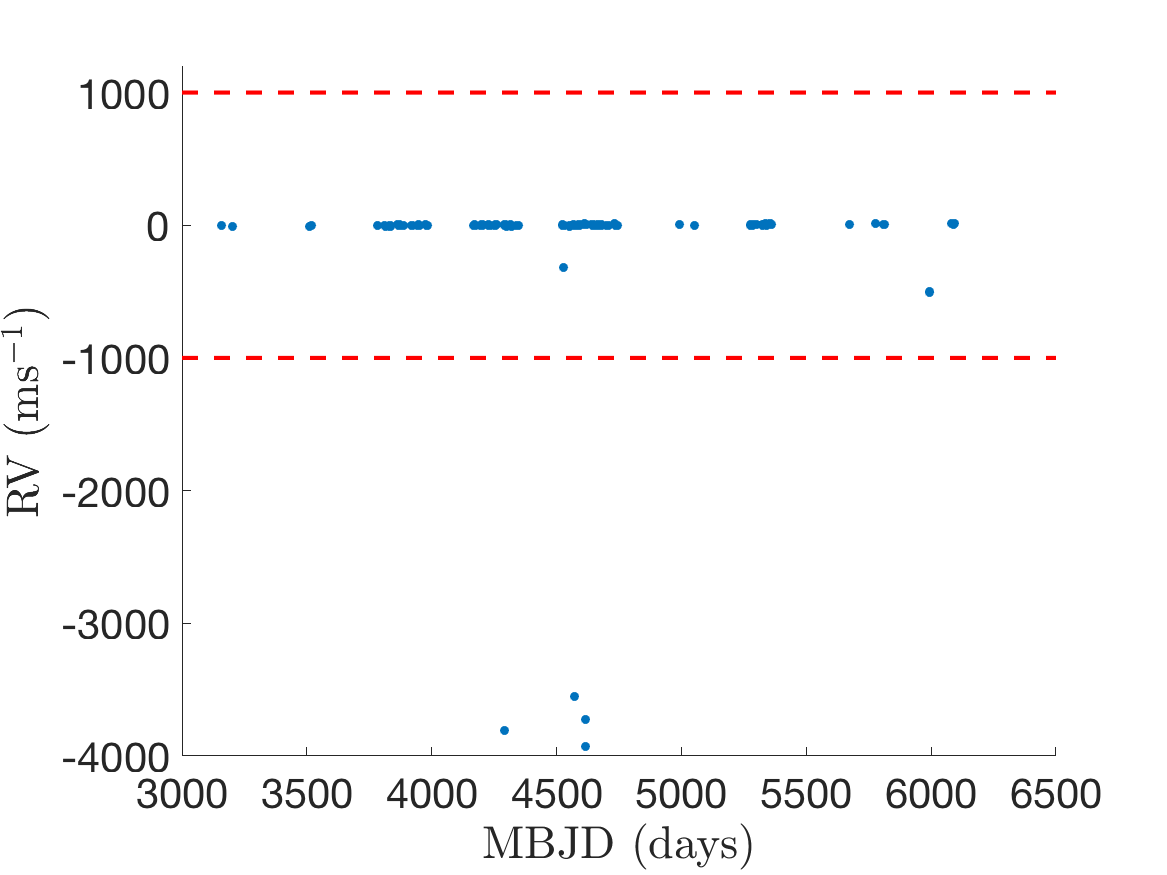
\includegraphics[width=0.8\textwidth]{GL667C_obs.png}
    \caption{Radial velocity of all observations of GL667C. The red dashed lines mark the $\pm$1 kms$^{-1}$ threshold from the median value.}
    \label{figGL667C_RV}
\end{figure}

Finally, all data taken after the 14th of May 2015 (MJD 2457165) were excluded due to an upgrade to the fibre cable from the ESO 3.6m telescope to the HARPS spectrograph \citep{2015LoCurto}. This was done to avoid any false signal in the analysis that might arise from the new fibre cable's performance or characteristics. While the post-change spectra would be of a higher quality, the majority of the spectra in the HARPS M-dwarf sample (as of the date of this work) were taken before the change, so the choice was made to exclude observations taken after the change. This might not be appropriate for a future analysis of a larger dataset continuing substantially more data from after the fibre change. 

\section{Method}
\label{secISVmethod}
\subsection{Data preparation}
\label{secISVdataprep}
\begin{figure}
    \centering
	\captionsetup{width=.8\textwidth}
	\subfloat[Five selected HARPS spectra of GL54.1. An arbitrary vertical offset has been added to each spectrum for clarity.]{\label{figGL541Int}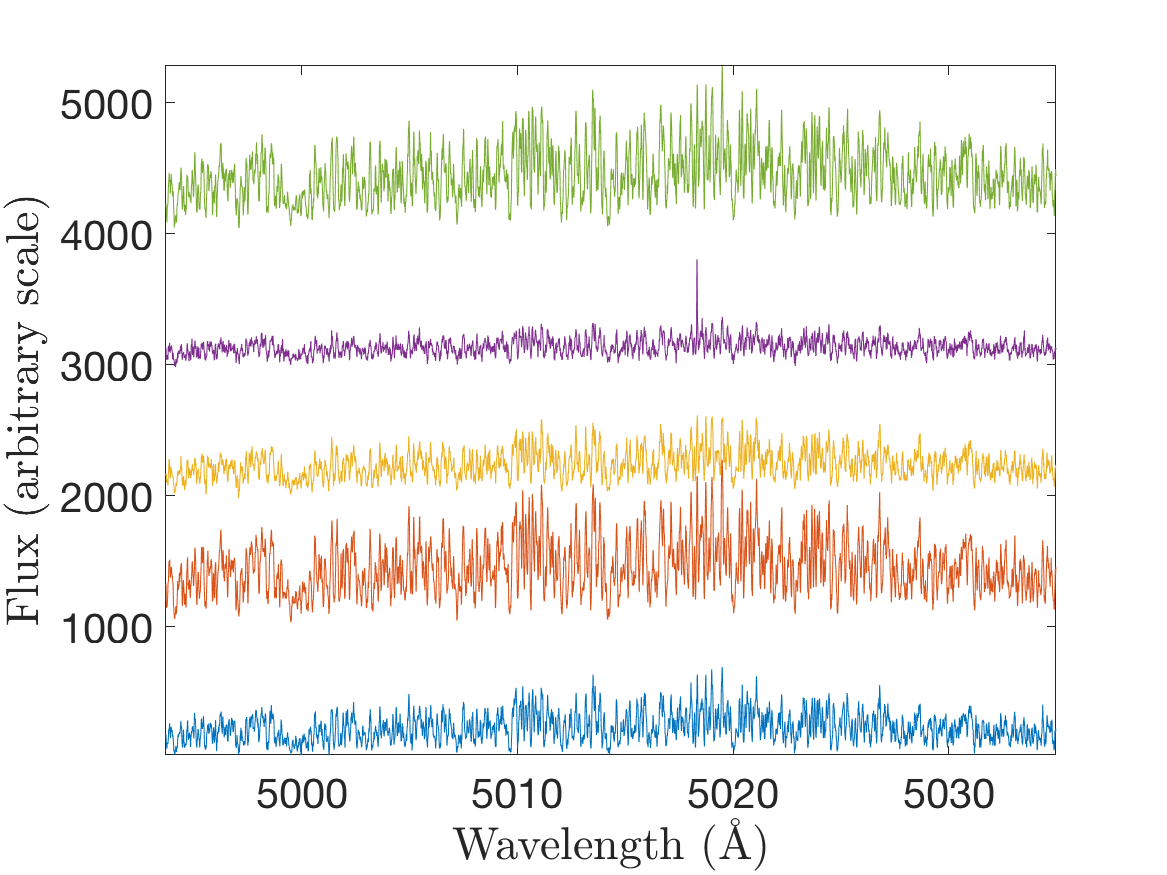
\includegraphics[width=0.8\textwidth]{Int.png}}\\
    \subfloat[The normalisation factors produced by dividing each spectrum in Figure\,\ref{figGL541Int} by the mean of all observations, again with arbitrary vertical offsets. The black lines are polynomials fitted to the normalisation factors. ]{\label{figGL541DevPoly}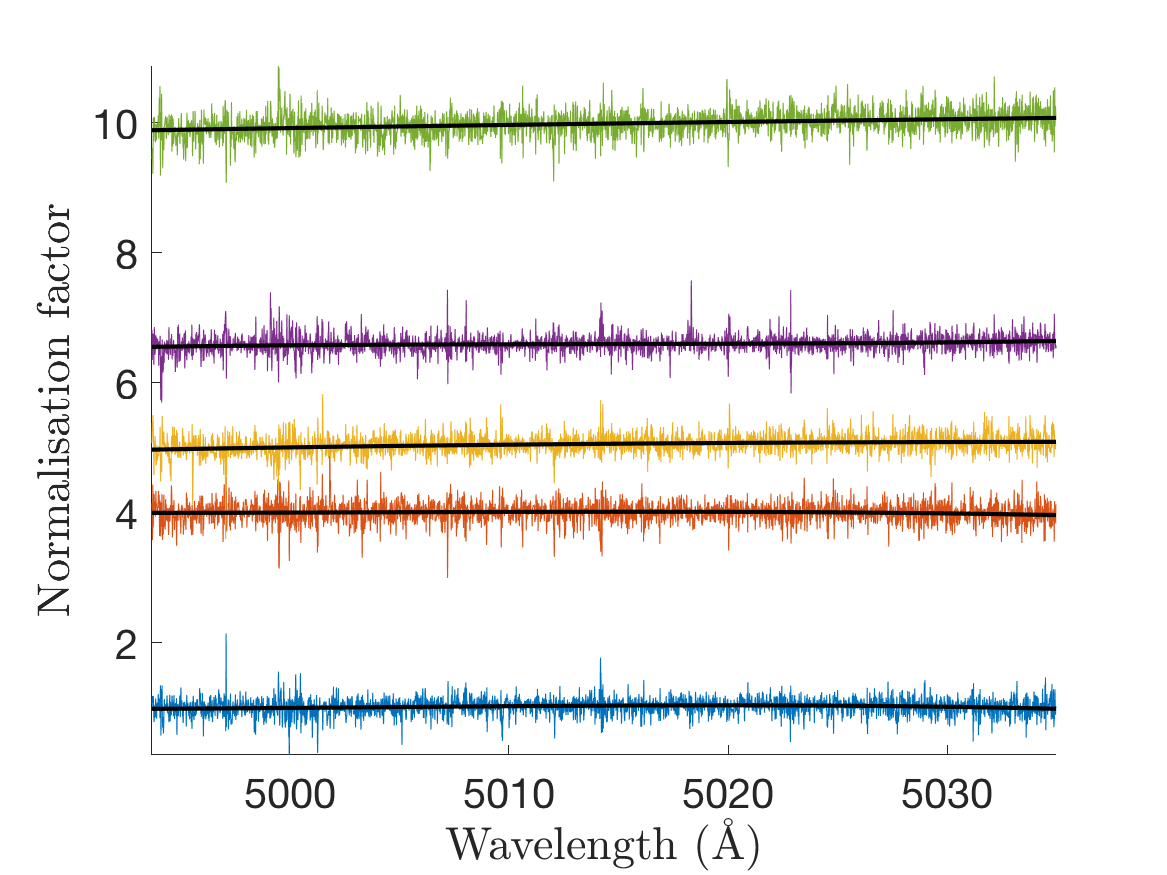
\includegraphics[width=0.8\textwidth]{DevPoly.png}}
    \caption{}
    \label{figISV_A}
\end{figure}

As both the observing conditions and barycentric correction will vary from observation to observation, the individual spectra needed to be both aligned to the same barycentric wavelength scale and normalised to the same relative flux. Each observation was corrected for the motion of the Earth around the Sun and the radial velocity of the star using the online version of \textit{barycorr} \citep{2014Wright} and the HARPS measured radial velocity.  During the velocity correction, all spectra were rebinned onto a velocity scale of 1x10$^{-6}$ ms$^{-1}$. The final step of the correction rebinned the spectra back into wavelength space. This produces a wavelength spacing of 0.0050\hbox{\AA} for order 40, to 0.0068\hbox{\AA} for order 71.\\

To highlight each step of the process, Figures\,\ref{figISV_A}-\ref{figISV_B} demonstrate the construction of the activity metric for GL54.1 using 89 observations. To normalise all observations of a given target to the same relative flux scale, each spectrum ($I(\lambda)$; Figure\,\ref{figGL541Int}) was divided by the mean of all the spectra to produce a normalisation factor $N(\lambda)$ (Equation\,\ref{eqNorm}; Figure\,\ref{figGL541DevPoly}) where $n$ is the total number of observations. To account for possible large-scale variations in $N(\lambda)$ over each order in each observation, $N(\lambda)$ was fitted with a third-order polynomial to create a smoothed normalisation function, $N_p(\lambda)$, seen as the black lines in Figure\,\ref{figGL541DevPoly}. This was then divided out of each raw spectrum to produce a normalised spectrum $I_{n}(\lambda)$ (Equation\,\ref{eqNew}; Figure\,\ref{figGL541New}).\\

\begin{table}[]
    \centering
    \begin{tabular}{|c|}
    \hline
    \vbox{\begin{equation}N(\lambda) = \frac{I(\lambda)}{\frac{1}{n}(\sum\limits_{i=1}^n I(\lambda)_{i})}\label{eqNorm}\end{equation}}\\
    \vbox{\begin{equation}I_{n}(\lambda) = \frac{I(\lambda)}{N_{p}(\lambda)}\label{eqNew}\end{equation}}\\
    \hline
    \end{tabular}
    \caption{Equations used to normalise stellar spectra in preparation of the production of an ISV spectrum.}
    \label{tabISVprep}
\end{table}
\subsection{Cosmic ray removal}
\label{secISVcosmic}
\begin{figure}
    \centering
	\captionsetup{width=.8\textwidth}
	\subfloat[Dividing each observation (Figure\,\ref{figGL541Int}) by its corresponding normalisation polynomial (Figure\,\ref{figGL541DevPoly}) removes variations between observations, putting all spectra onto the same scale.]{\label{figGL541New}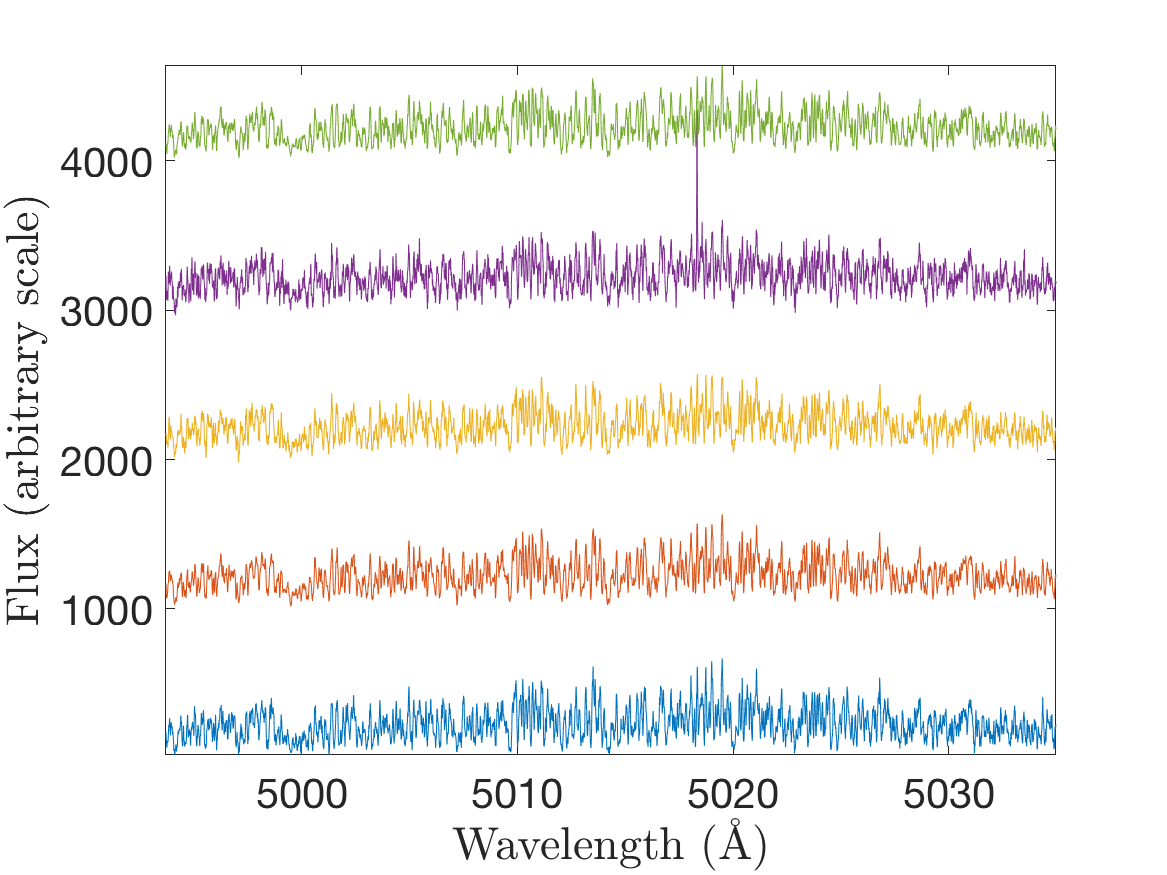
\includegraphics[width=0.8\textwidth]{New.png}}\\
    \subfloat[The spectra from Figure\,\ref{figGL541New} after clipping outliers above the $6\sigma$ level. The cosmic ray at $\sim$5018\,\hbox{\AA} in the purple spectrum has been removed.]{\label{figGL541Cosmic}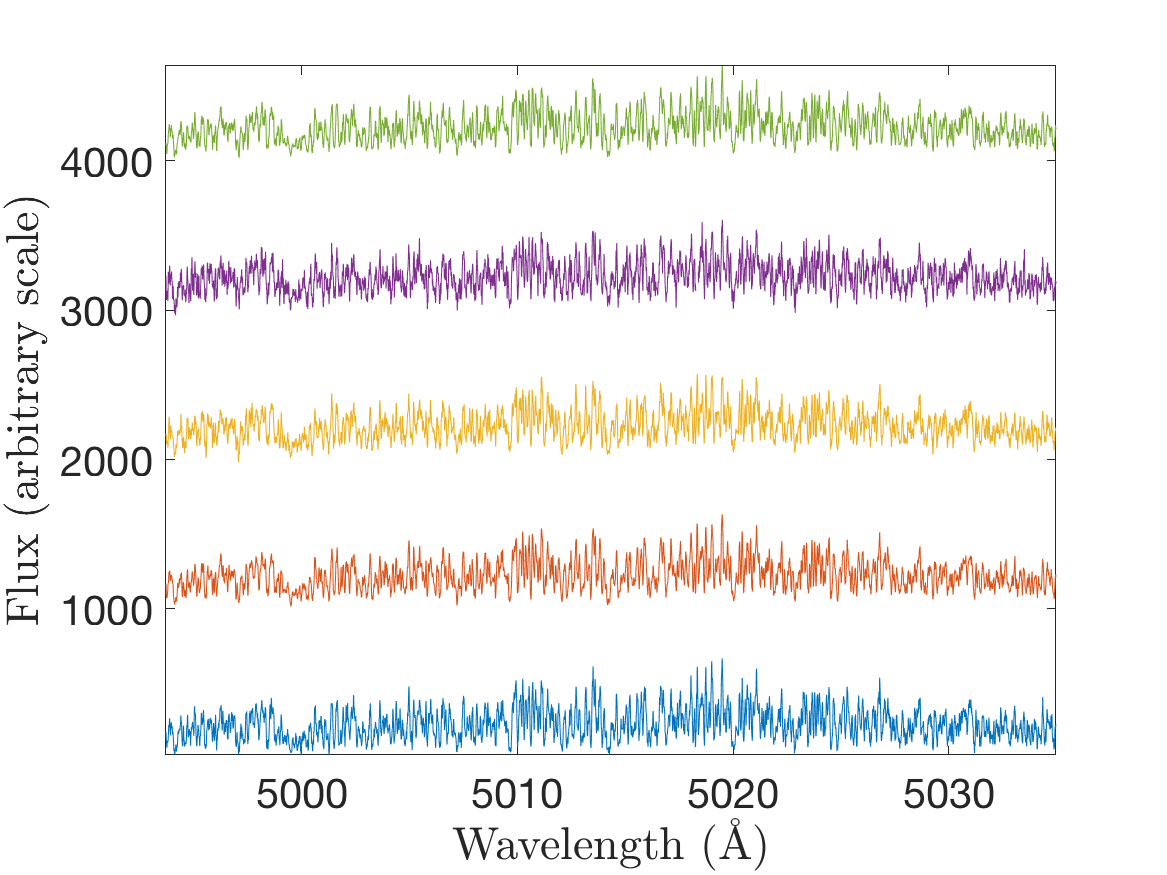
\includegraphics[width=0.8\textwidth]{Cos.png}}
    \caption{}
\end{figure}

Cosmic rays are an obvious potential source of false-positive spectral variability and the impacted data points needed to be masked to exclude them from the subsequent calculations. If the exposure time is short, comparing multiple sequential observations can identify the pixels undergoing a substantial short-term change and they can be replaced by the mean of the other observations \citep{2000Fixsen}. Laplacian edge detection can also be used to identify cosmic rays \citep{2001VanDokkum}. Cosmic ray imprinted pixels in the data were identified by applying an iterative 6$\sigma$ clip across all observations at each wavelength. To ensure the entire cosmic ray was removed, all pixels within one minimum resolvable element on either side of an identified pixel were also masked. From the resolution of the spectrograph (R = 120,000) and the wavelength range used, the minimum resolvable element ranged from 0.04\hbox{\AA} to 0.06\hbox{\AA}. To ensure that the entire cosmic ray was removed, the larger value was used. This value is used as the FWHM of every HARPS ISV spectral line throughout the rest of this work. For each potential cosmic ray. all pixel values within one minimum resolvable element on either side of an identified pixel had their values set to NaN in that particular spectrum. The cosmic ray seen in the purple spectrum of Figure\,\ref{figGL541New} is masked in the cleaned spectrum, $I_{c}(\lambda)$, in Figure\,\ref{figGL541Cosmic}.

\subsection{Determining the ISV}
\label{secISVdetermine}
\begin{figure}
    \centering
	\captionsetup{width=.8\textwidth}
	\subfloat[The mean of all cosmic ray cleaned spectra for GL54.1 in order 40. ]{\label{figGL541MeanISV}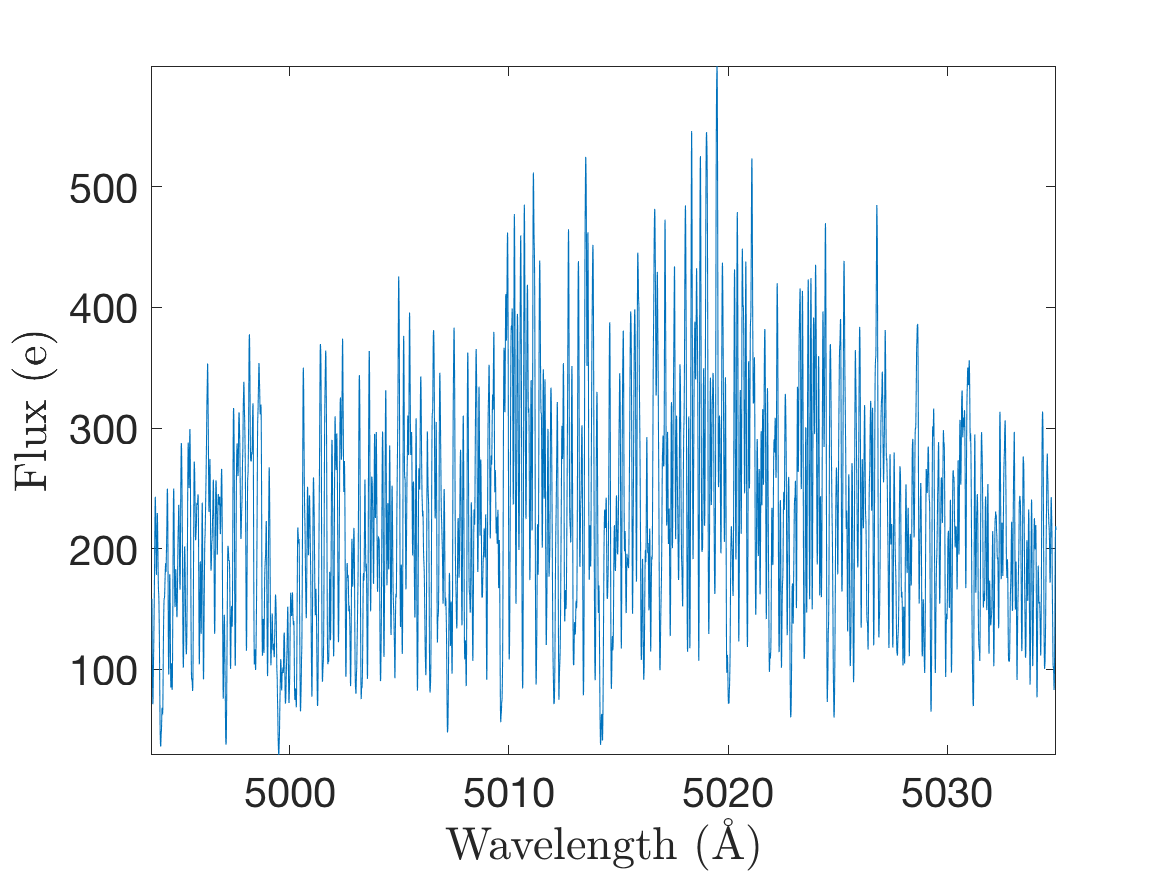
\includegraphics[width=0.8\textwidth]{MeanCos.png}}\\
    \subfloat[The weighting of each pixel in the individual spectra of GL54.1 in order 40.]{\label{figGL541WeightISV}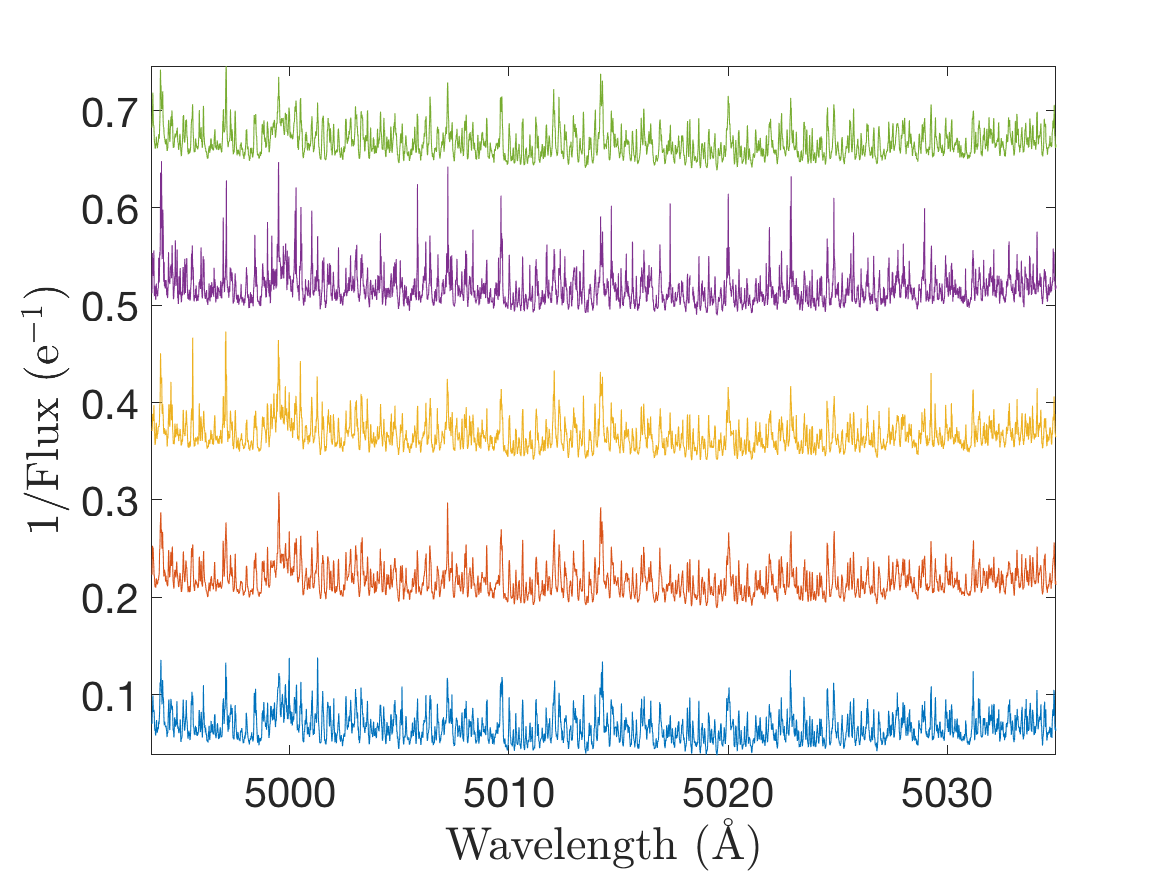
\includegraphics[width=0.8\textwidth]{WeightCos.png}}
    \caption{}
\end{figure}

\begin{figure}
    \centering
	\captionsetup{width=.8\textwidth}
	\subfloat[The weighted standard deviation as a function of wavelength across the GL54.1 spectra in order 40.]{\label{figGL541ISV1}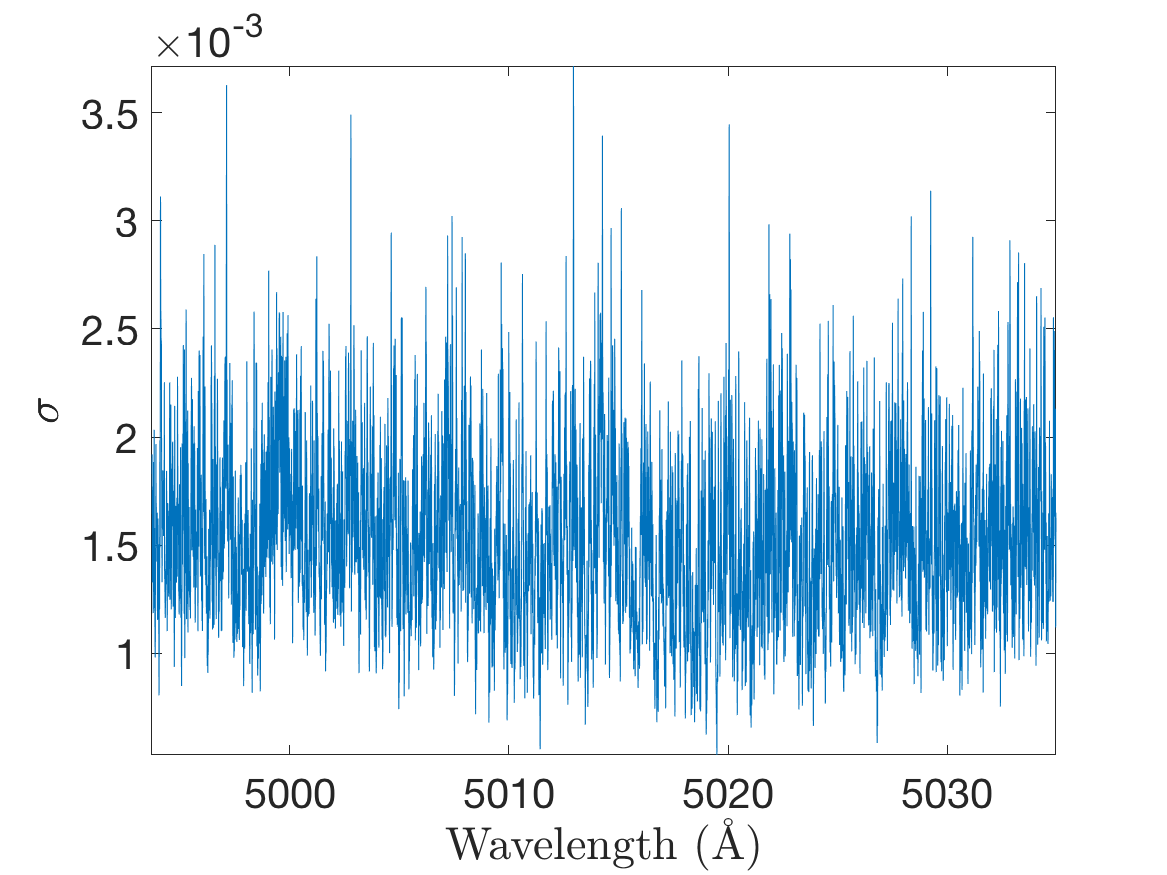
\includegraphics[width=0.8\textwidth]{ISV1.png}}\\
    \subfloat[The resulting ISV in order 40 for GL54.1.]{\label{figGL541ISV2}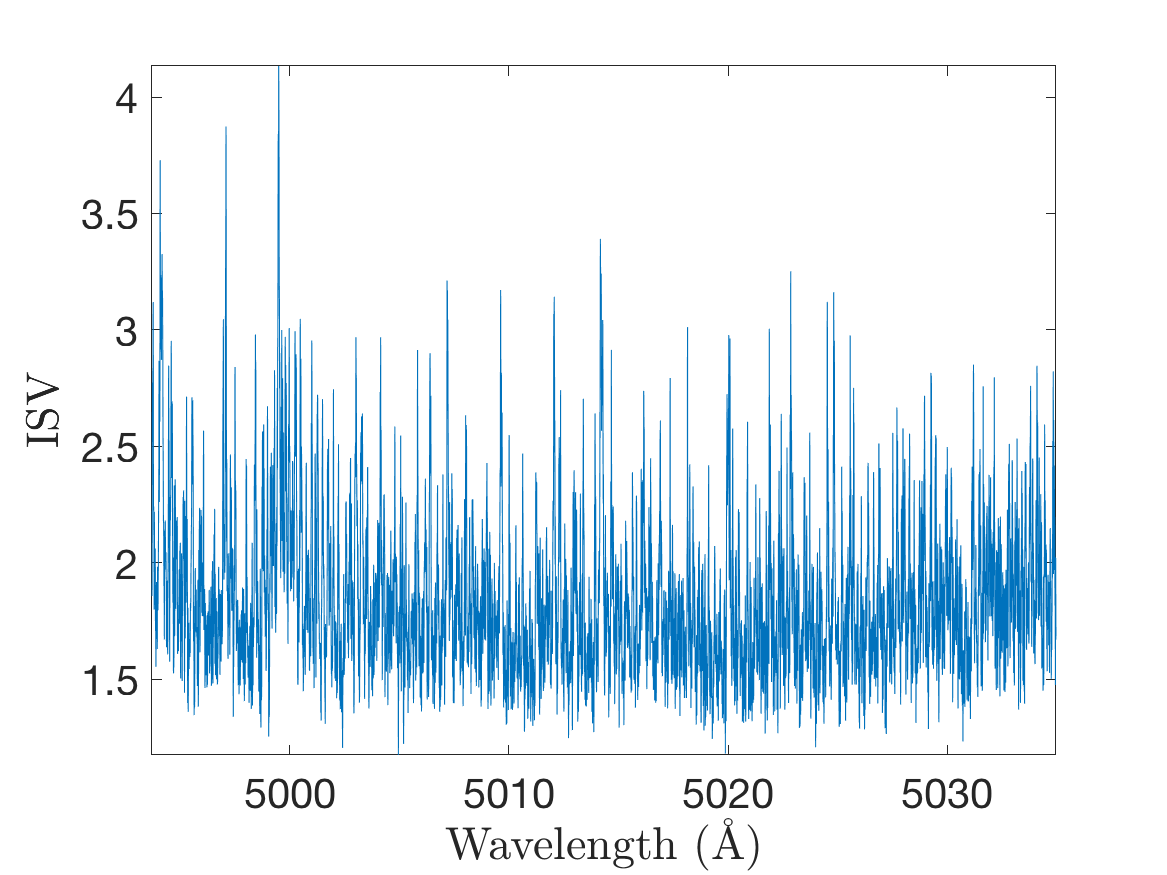
\includegraphics[width=0.8\textwidth]{ISV2.png}}
    \caption{}
    \label{figISV_B}
\end{figure}

The Intrinsic Stellar Variability (ISV) metric is defined as the ratio of the observed RMS scatter to the instrumental RMS scatter, specifically the weighted standard deviation across all observations for each pixel after cosmic ray cleaning (observed scatter), and the mean combination of the photometric uncertainty and read noise (instrumental scatter). For this, a mean spectrum needed to be produced and a weighting needed to be determined for every pixel. The mean spectrum, $I_{m}(\lambda)$, is obtained from the cosmic ray cleaned spectra (Equation\,\ref{eqMean}; Figure\,\ref{figGL541MeanISV}). The number of observations for a specific wavelength will vary due to the cosmic ray cleaning, therefore $m$ in Equations\,\ref{eqMean}, \ref{eqSigV}, and \ref{eqSigI}, is the number of observations for a specific wavelength. The weighting was taken as the inverse of the instrumental uncertainties (Equation\,\ref{eqWeight}). In the absence of a HARPS provided uncertainty estimate, one was estimated as the sum of the Poisson noise, $\sqrt{\abs{I(\lambda)}}$, and read noise, $R$, for each pixel, scaled by the normalisation factor polynomial (Equation\,\ref{eqPhoton}). The weighting of the 5 example spectra of GL54.1 can be seen in Figure\,\ref{figGL541WeightISV}. The observed RMS scatter is then the weighted standard deviation (Equation\,\ref{eqSigV}; Figure\,\ref{figGL541ISV1}), and the instrumental RMS scatter is the mean of the instrumental uncertainties across multiple observations for each wavelength (Equation\,\ref{eqSigI}), and the ISV is the ratio of the two (Equation\,\ref{eqISV2}; Figure\,\ref{figGL541ISV2}). 

%\begin{equation}
%    I_{m}(\lambda) = \frac{1}{m}(\sum\limits_{i=1}^m I_{c}(\lambda)(i))
%    \label{eqMean}
%\end{equation}

%\begin{equation}
%    \sigma_{i}(\lambda) = \frac{\sqrt{I(\lambda)+R^2}}{N_p(\lambda)}
%    \label{eqPhoton}
%\end{equation}

%\begin{equation}
%    W(\lambda) = \frac{1}{\sigma_{i}(\lambda)}
%    \label{eqWeight}
%\end{equation}

%\begin{equation}
%   \sigma_{v}(\lambda) =  \sqrt{\frac{\sum\limits_{i=1}^m W(\lambda)_{i}(I_{c}(\lambda)(i)-I_{m}(\lambda))^2}{\frac{m-1}{m}\sum\limits_{i=1}^m W(\lambda)_{i}}}
%   \label{eqSigV}
%\end{equation}

%\begin{equation}
%    \bar{\sigma_i}(\lambda) = \sqrt{\frac{\sum\limits_{i=1}^m\sigma_{i}^2}{m}}
%    \label{eqSigI}
%\end{equation}

%\begin{equation}
%    ISV(\lambda) = \frac{\sigma_{v}(\lambda)}{\bar{\sigma_i}(\lambda)}
%    \label{eqISV2}
%\end{equation}

\begin{table}[]
    \centering
    \begin{tabular}{|c|}
    \hline
    \vbox{\begin{equation}I_{m}(\lambda) = \frac{1}{m}(\sum\limits_{i=1}^m I_{c}(\lambda)(i))\label{eqMean}\end{equation}}\\
    \vbox{\begin{equation}\sigma_{i}(\lambda) = \frac{\sqrt{I(\lambda)+R^2}}{N_p(\lambda)}\label{eqPhoton}\end{equation}}\\
    \vbox{\begin{equation}W(\lambda) = \frac{1}{\sigma_{i}(\lambda)}\label{eqWeight}\end{equation}}\\
    \vbox{\begin{equation}\sigma_{v}(\lambda) =  \sqrt{\frac{\sum\limits_{i=1}^m W(\lambda)_{i}(I_{c}(\lambda)(i)-I_{m}(\lambda))^2}{\frac{m-1}{m}\sum\limits_{i=1}^m W(\lambda)_{i}}}\label{eqSigV}\end{equation}}\\
    \vbox{\begin{equation}\bar{\sigma_i}(\lambda) = \sqrt{\frac{\sum\limits_{i=1}^m\sigma_{i}^2}{m}}\label{eqSigI}\end{equation}}\\
    \vbox{\begin{equation}ISV(\lambda) = \frac{\sigma_{v}(\lambda)}{\bar{\sigma_i}(\lambda)}\label{eqISV2}\end{equation}}\\
    \hline
    \end{tabular}
    \caption{Equations used in the production of an ISV spectrum.}
    \label{tabISVeqautions}
\end{table}
\subsection{ISV features}
\label{secISVfeatures}
ISV ``spectra'' have been produced for every star in the sample and plots are presented in Section\,\ref{secResults}. Broadly, the ISV is a dimensionless quantity that measures how much the flux at a given wavelength varies compared to other wavelengths. A low-level variation will occur across all wavelengths due to photon noise, low-level stellar variability, and instrumental uncertainty, which will be referred to as the ``baseline'' noise in the ISV. The ISV plot of GL479 (Figure\,\ref{figGL479ISVfull}) contains a baseline noise that spans an ISV of 1-2. The features of interest are the wavelengths that vary significantly more than the baseline noise. These will be referred to as ISV lines, and once they are confirmed to be produced by variability in a stellar spectral line, they will be called ISV spectral lines. Figure\,\ref{figGL551line} shows the original spectra and the calculated ISV in the wavelength region of an example Fe\textsc{I} absorption line at $\lambda$ = 5269.537\hbox{\AA}  for the star GL551. The spectral line is clearly varying between observations, from minor absorption to clear emission, and the ISV is detecting this variation. \\

\begin{figure}[!h]
    \centering
	\captionsetup{width=.8\textwidth}
	\subfloat[An ISV plot for GL479 across multiple orders.]{\label{figGL479ISVfull}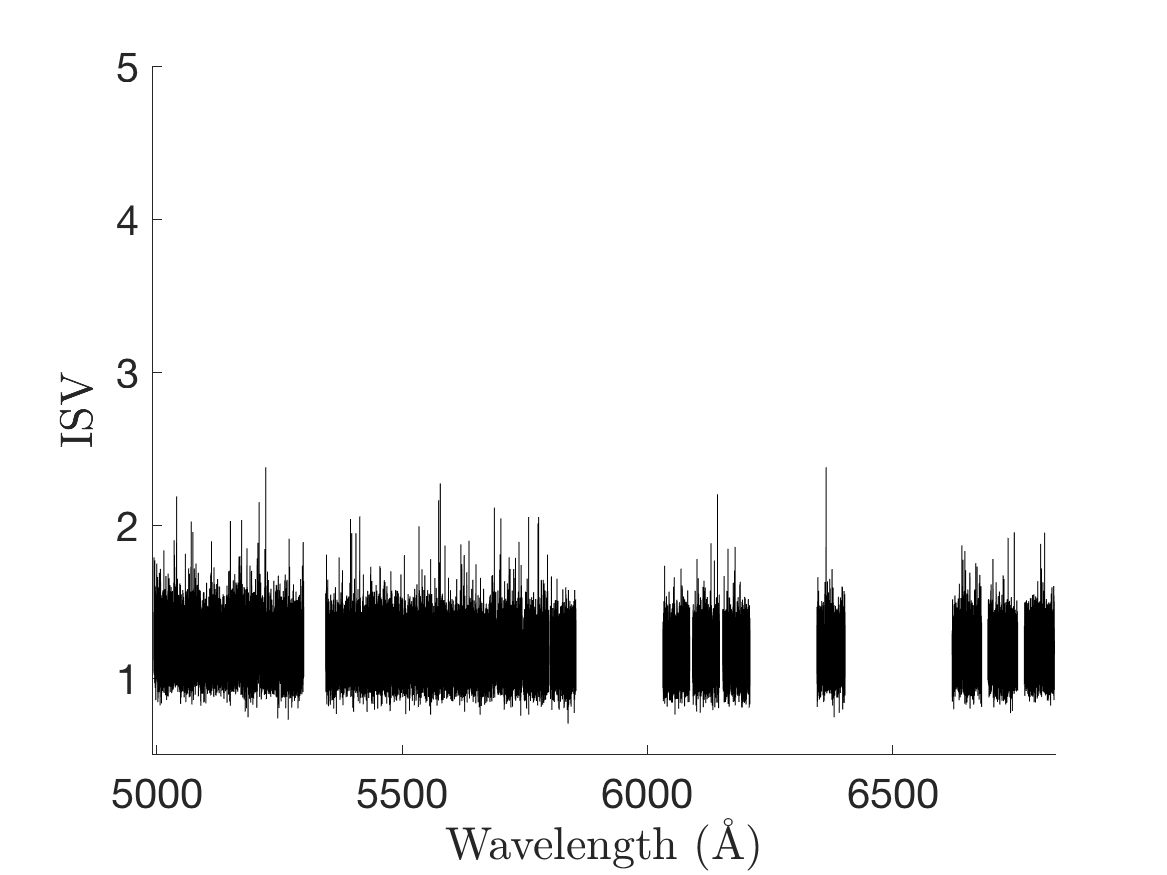
\includegraphics[width=0.8\textwidth]{Gl479_comparison.png}}\\
    \captionsetup{width=.8\textwidth}
	\subfloat[(top) A varying Fe\textsc{I} line present in the spectra of GL551. (bottom) The ISV for GL551 in the same wavelength range.]{\label{figGL551line}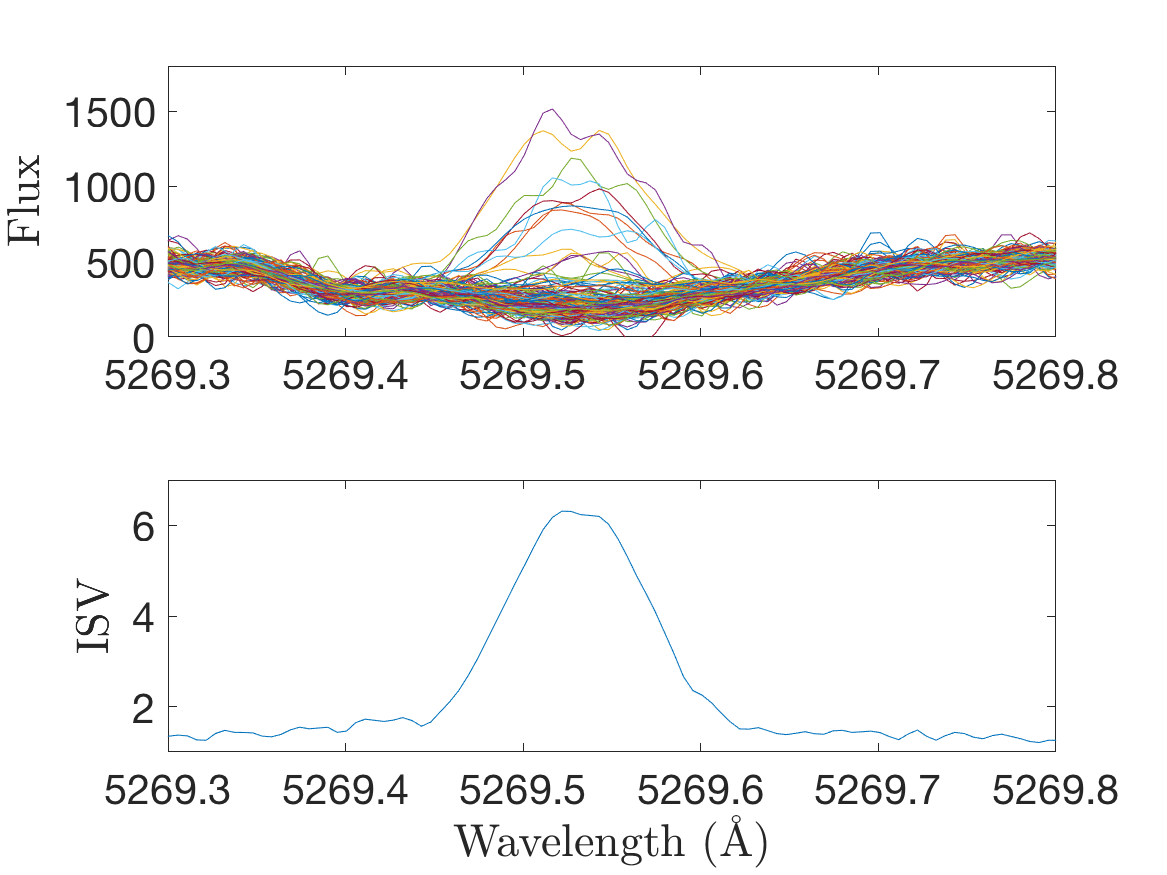
\includegraphics[width=0.8\textwidth]{Gl551_line.png}}
    \caption{}
\end{figure}

\begin{figure}[!h]
    \centering
	\captionsetup{width=.8\textwidth}
	\subfloat[An ISV plot for GL555 produced from 10 observations. The baseline noise of this ISV is particularly large.]{\label{figGL555ISVfull}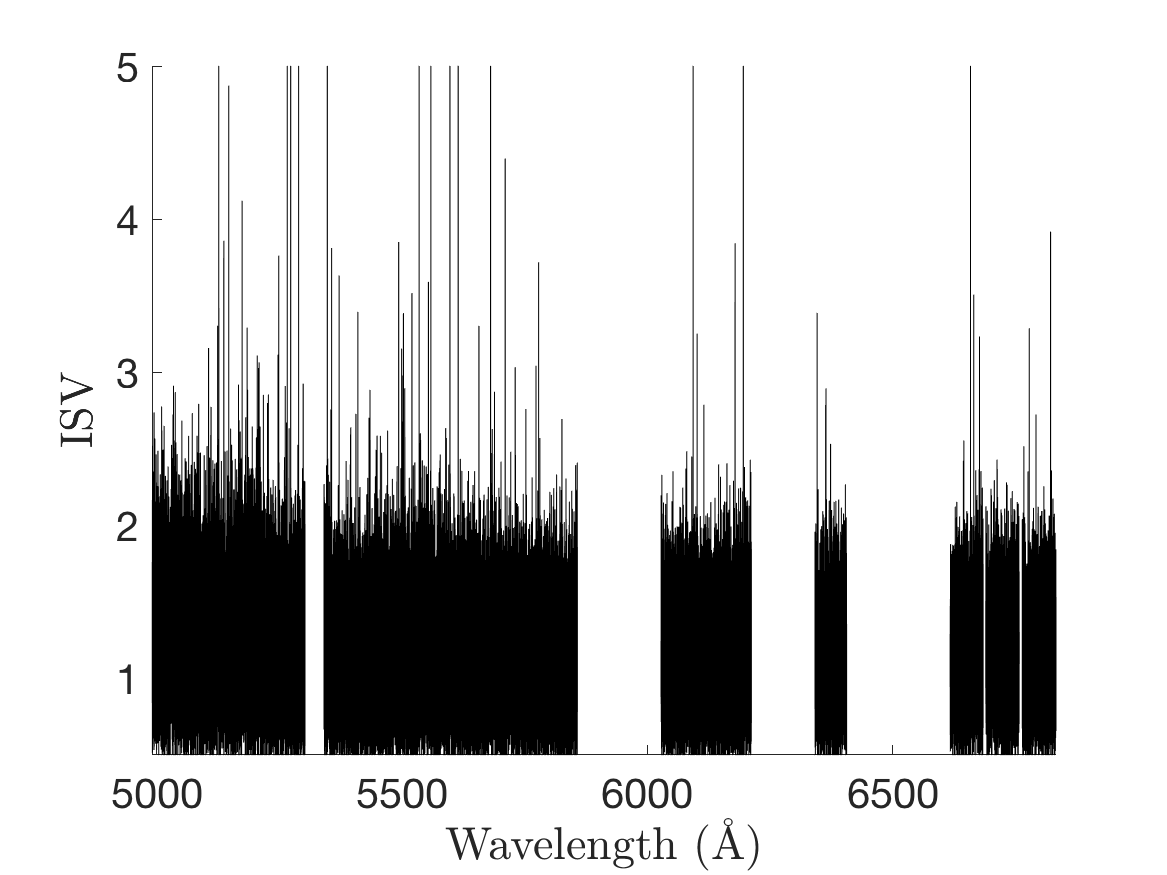
\includegraphics[width=0.8\textwidth]{Gl555_comparison.png}}\\
    \subfloat[A histogram of the ISV values for GL479 (brown) and GL555 (blue).]{\label{figISVhist}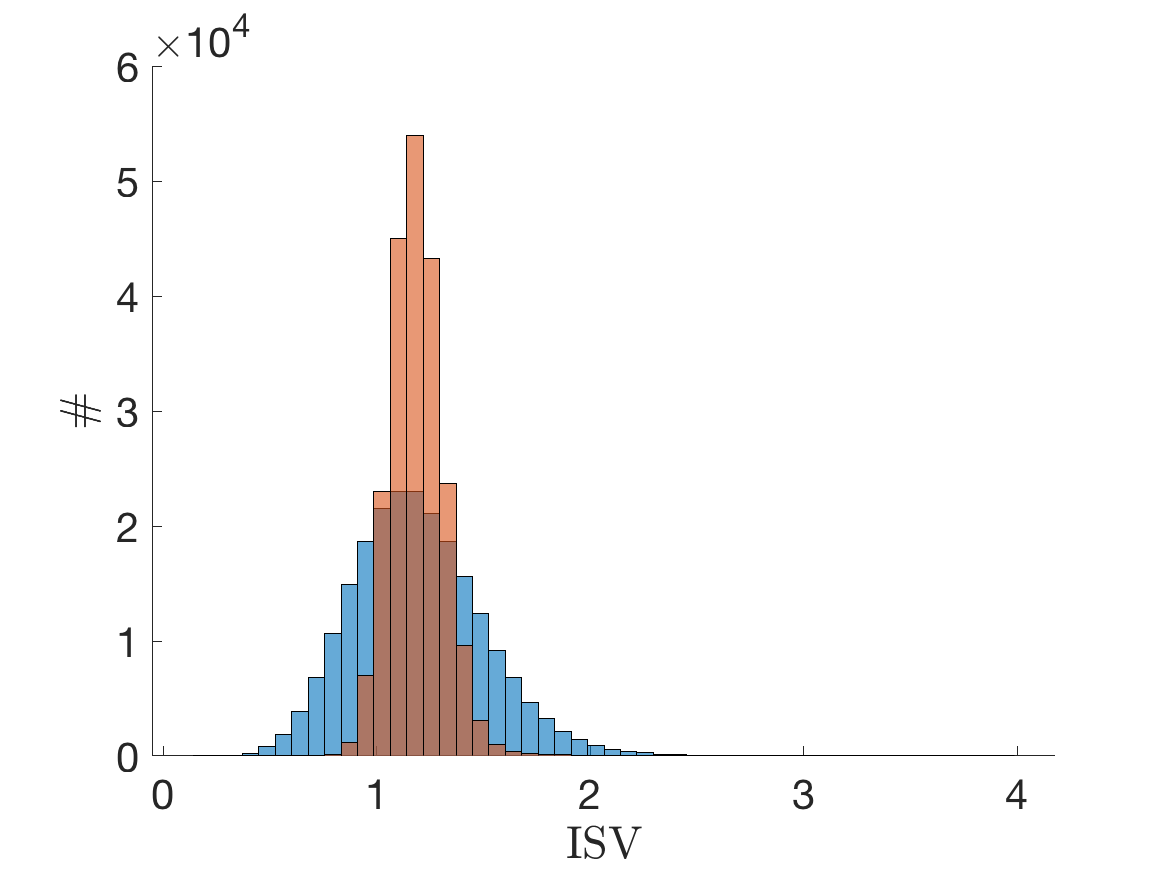
\includegraphics[width=0.8\textwidth]{Gl555_Gl479_hist.png}}
    \caption{}
\end{figure}

A typical ISV line has a width of 0.1-0.2\,\AA. If an ISV line is small relative to the baseline noise, it will not be detectable above that threshold. The main factors that will determine the level of the baseline noise in the ISV are the signal to noise ratio in the spectrum and the number of observations used to create the ISV. Comparing the ISV spectra of GL479 (Figure\,\ref{figGL479ISVfull}) with GL555 (Figure\,\ref{figGL555ISVfull}) it can be seen that the the baseline noise for GL555 is roughly 2 times as broad as for GL479, with a slightly higher mean, and Figure\,\ref{figISVhist} compares the distributions of the ISV values for the two stars. GL479 has an apparent magnitude of V\,=\,10.66 and its ISV used 58 observations. GL555 is almost a magnitude fainter (V\,=\,11.32) and its ISV is constructed from only 10 observations. Both stars had exposure times of 900s. For N observations per star and assuming that the distribution of ISV values is Gaussian, the magnitude of the baseline noise, W, can be estimated as 2$\sigma$ from the mean of the ISV distribution (i.e. the 2.3 and 95.4 percentile). Figure\,\ref{figBaselineComparison} shows an inverse linear relationship between the magnitude of the baseline noise and the square root of the number of observations. M-dwarfs are not particularly luminous stars, so to increase the signal-to-noise would require longer exposure times. As the data used in this work is a public data release, nothing can be done to change the exposure times or add data at this point. However, requiring a minimum number of observations per star can ensure that the baseline noise will be sufficiently weak that a strong ISV line will be prominent above it. After a visual examination of multiple ISV plots, a minimum of 20 observations was adopted, reducing the sample to 49 stars.\\

\begin{figure}
    \centering
	\captionsetup{width=.8\textwidth}
	\subfloat[A plot of the number of observations used to calculate ISV versus the magnitude of the baseline noise for all the M-dwarfs in the sample.]{\label{figBaselineComparison}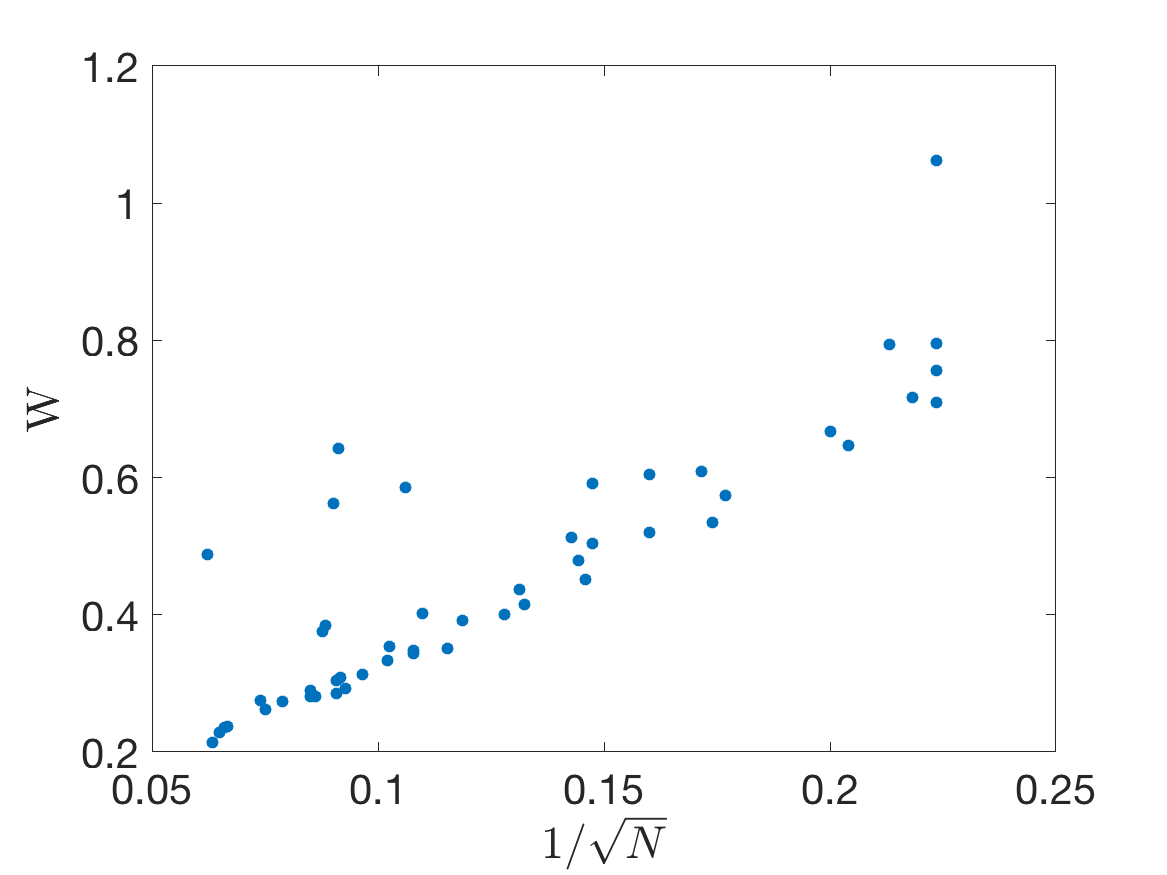
\includegraphics[width=0.8\textwidth]{Baseline_correlation.png}}
	\captionsetup{width=.8\textwidth}
	\subfloat[The baseline noise of GL551 varies significantly with wavelength.]{\label{figGL551}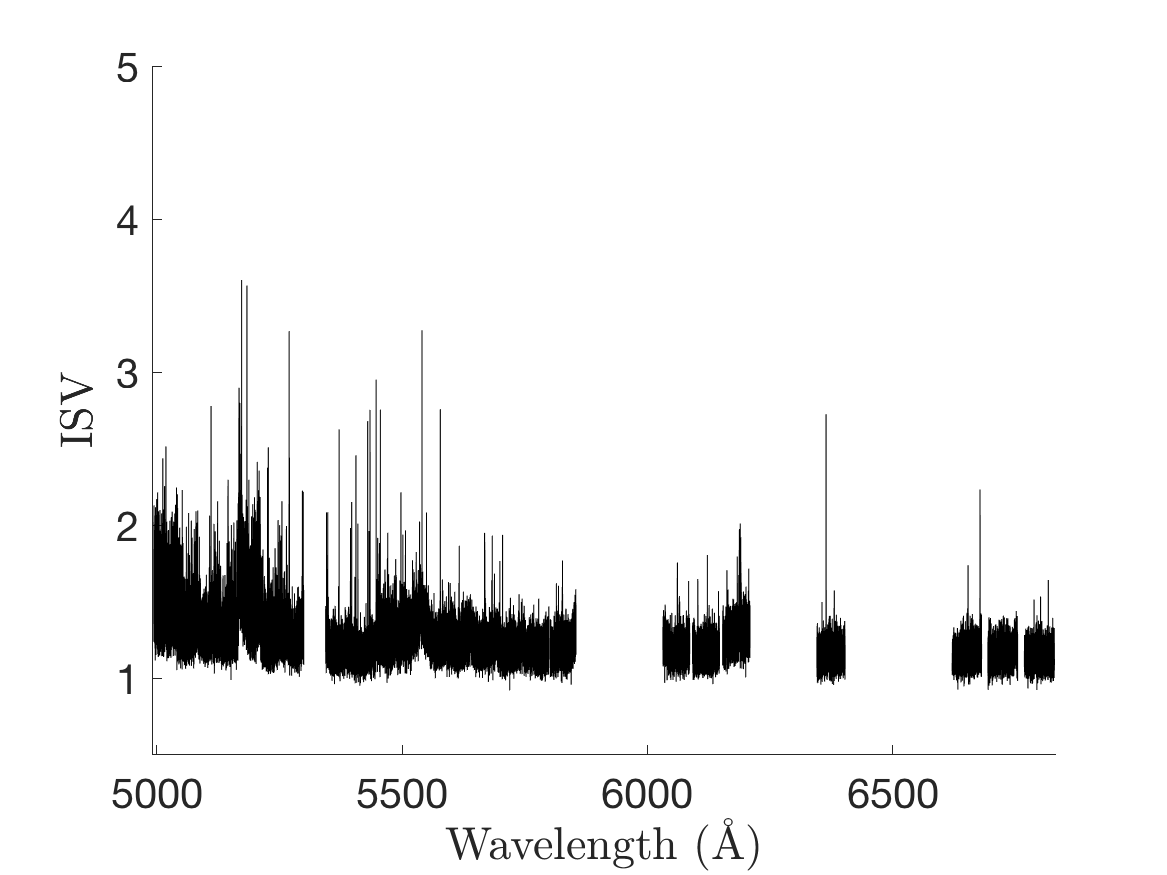
\includegraphics[width=0.8\textwidth]{Gl551_comparison.png}}
    \caption{}
\end{figure}

The baseline noise was generally wavelength independent, but in a few cases was seen to vary with wavelength. Generally this happened for the the cooler and fainter M-dwarfs. If the ISV plots of GL479 (Figure\,\ref{figGL479ISVfull}) and GL551 (Figure\,\ref{figGL551}) are compared it can be seen that GL479 has a reasonably flat baseline noise, but that several orders in GL551 appear ``curved'' (particularly at shorter wavelengths) and that there are offsets between some orders. A visual inspection of the ISV spectra produced from the entire sample found that these `non-flat' orders were present in several stars, often in the blue orders. To identify the cause of these non-flat orders required investigating the the development of the ISV at each step in the process. Figure\,\ref{figordercurve} presents the flux, weights, observed RMS scatter, instrumental RMS scatter, and ISV for one order of GL388 and GL54.1. These two stars have the same subtype (M4), and both have a mix of 600s and 900s exposure times. The major difference between them is their apparent magnitudes (V\,=\,9.52 and V\,=\,12.07) which lead to a significant difference in signal-to-noise per pixel at the centre of order 40 (30.5 and 6.7). The chosen order appears to have 1-2 molecular bands spanning 5165-5185 \hbox{\AA} and another band bluewards of 5200 \hbox{\AA}. The weighting is stronger at those wavelengths, compared to the rest of the wavelengths in the order, for both stars. However, due to the lower flux from GL54.1, this increase in weighting is more pronounced than for GL388. When the observed and instrumental RMS scatter for each star are compared, the difference in the weighting becomes apparent. For GL388 the observed RMS scatter has a slightly greater magnitude than the instrumental RMS scatter, but has a generally similar distribution, producing a reasonably flat baseline noise in the ISV. A similar situation occurs for GL54.1, but only in the small wavelength region with no observable molecular bands. Across the molecular band affected wavelengths, the observed and instrumental RMS scatter for GL54.1 diverge significantly, producing an increased ISV at those wavelengths. Clearly the difference in flux is amplifying the imprinted molecular bands in the dimmer star. This changing baseline noise can complicate the identification of which variation above the baseline noise is significant. This is further discussed in Section\,\ref{secISVlines}.\\

\begin{figure}
    \hspace{-2cm}
	\captionsetup{width=.8\textwidth}
	\subfloat[]{\label{figGL388ordercurve}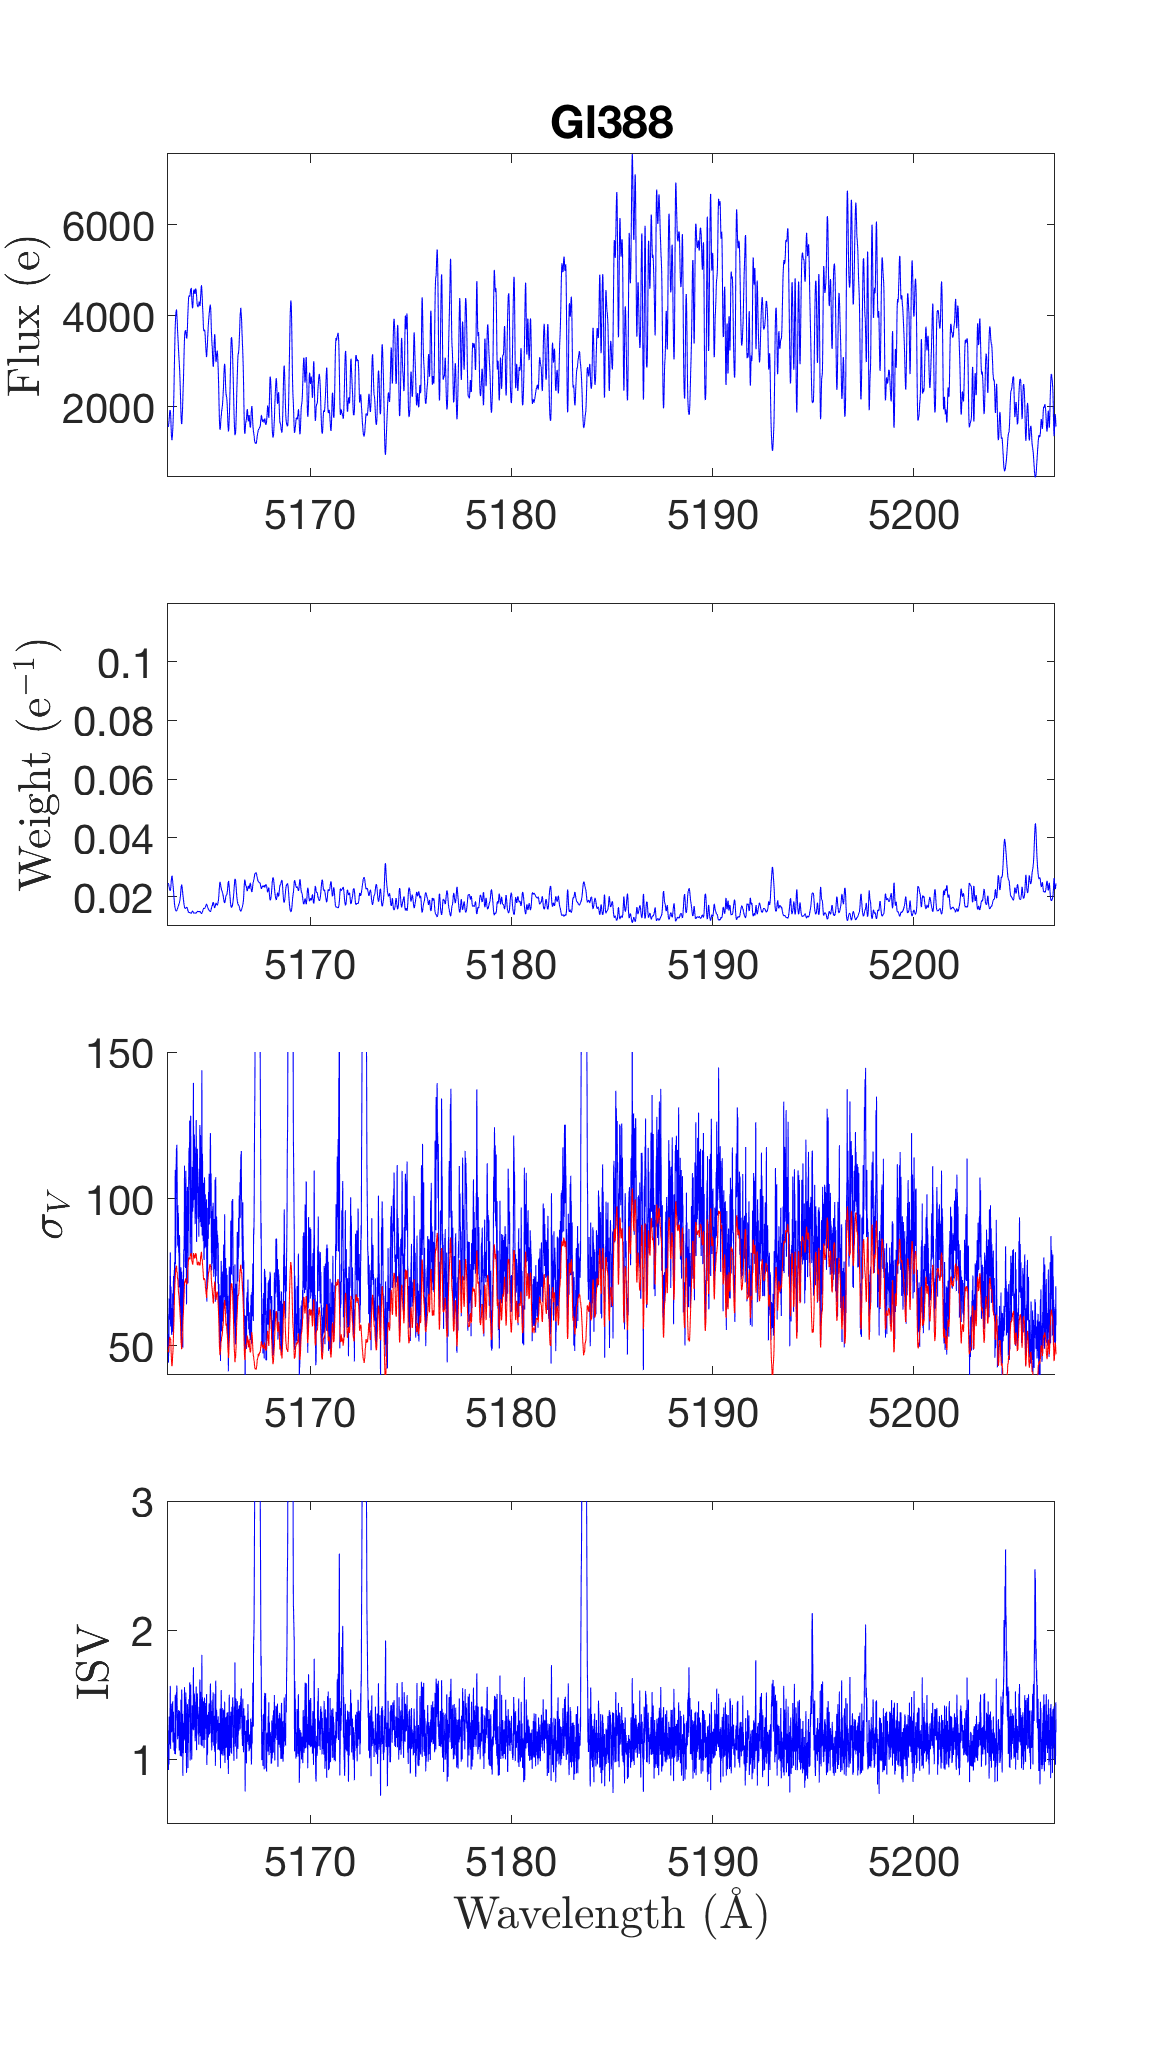
\includegraphics[width=0.6\textwidth]{Gl388_order_curve.png}}
	\subfloat[]{\label{figGL541ordercurve}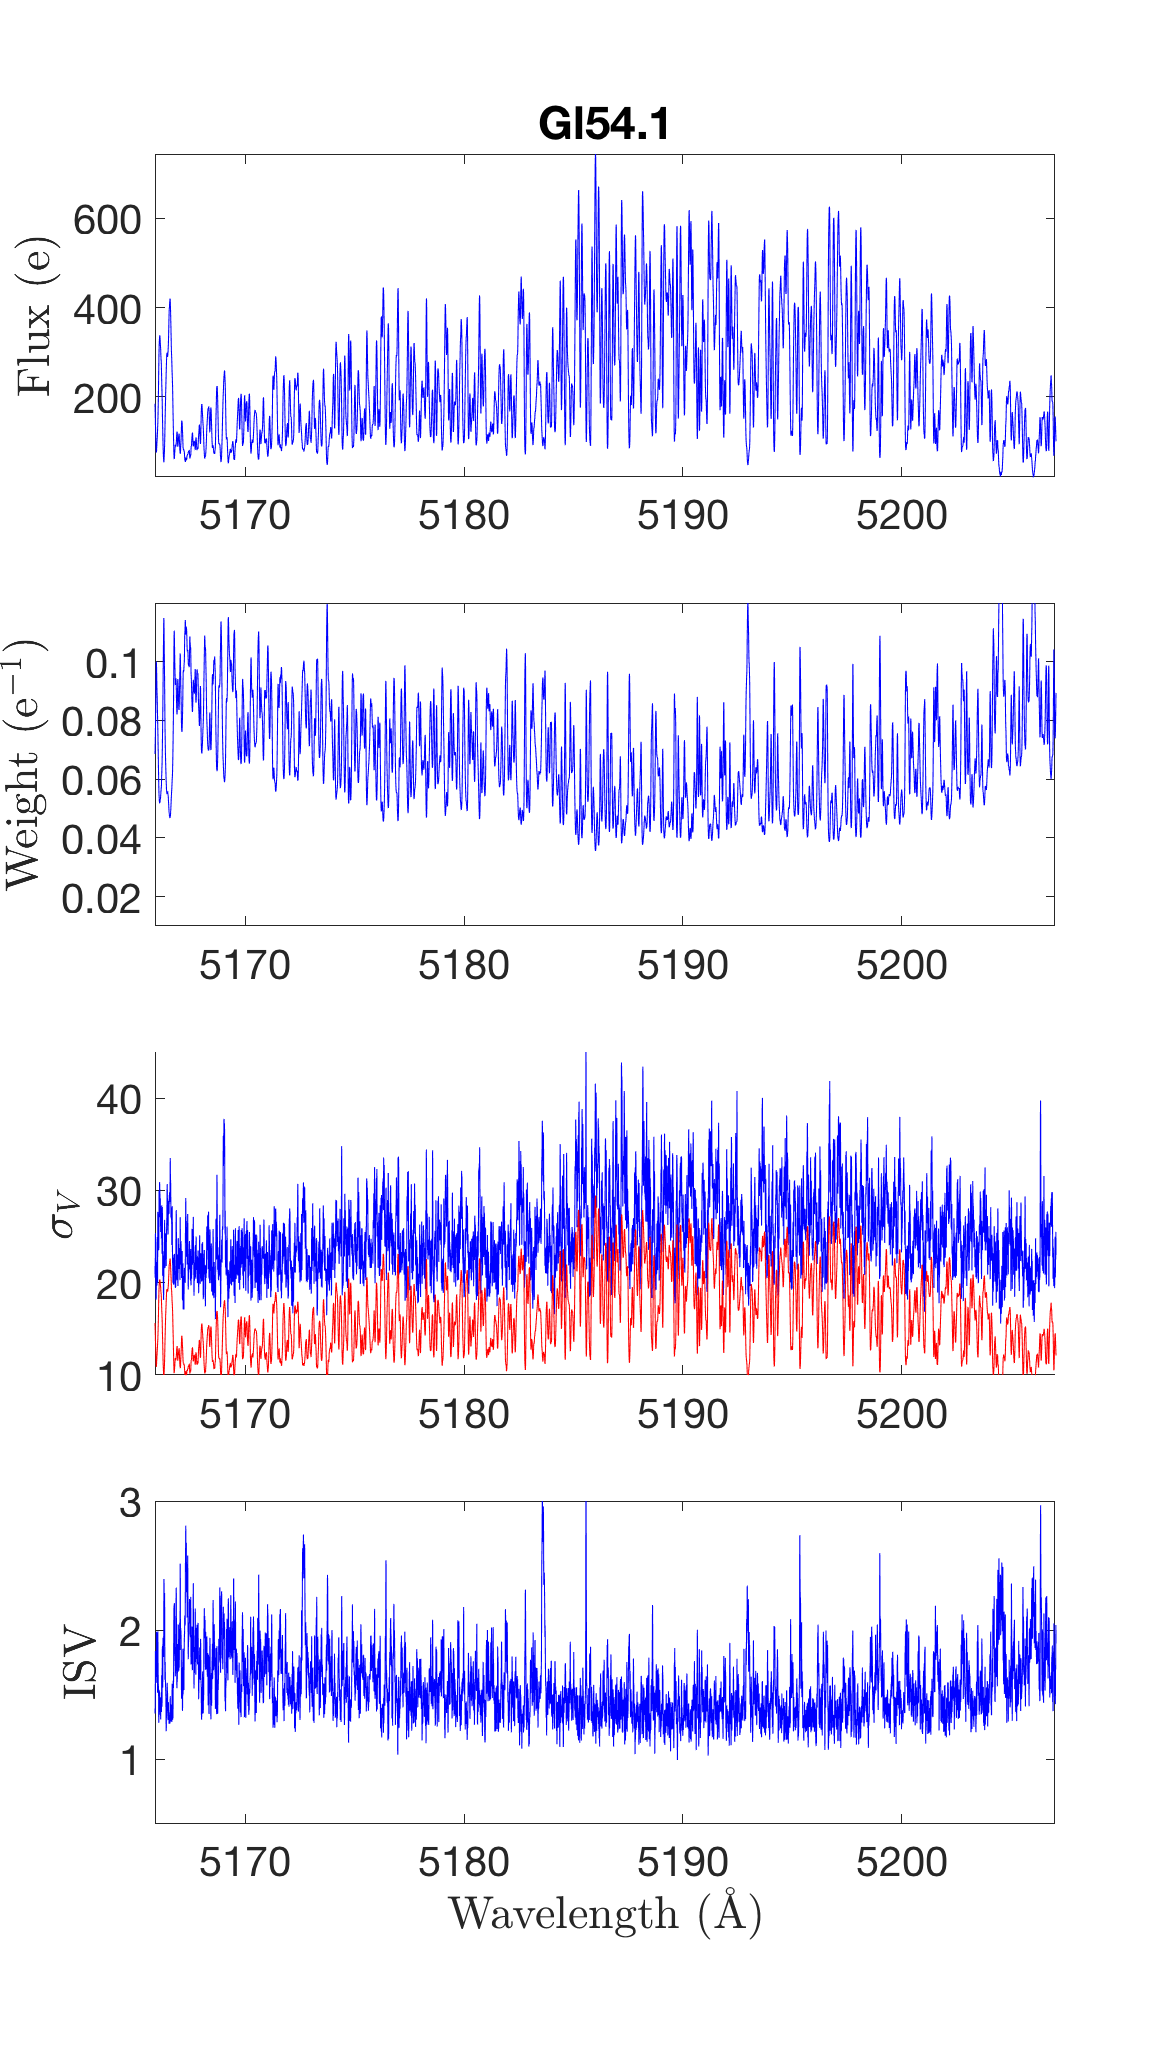
\includegraphics[width=0.6\textwidth]{Gl54_1_order_curve.png}}
    \caption{Plots of the flux (1st panel), weights (2nd panel), RMS and instrumental scatter (3rd panel), and ISV (4th panel) for GL388 and GL54.1. The observed RMS scatter is shown in blue and the instrumental RMS scatter is in red.}
    \label{figordercurve}
\end{figure}

One last feature to mention is an elevation of the last (reddest) order in some stars. When this occurs, the order's ISV spectrum has a similar level of baseline noise to the preceding order, but all variation is $\sim$0.1 greater. Due to the low levels of flux in the reddest order, and the typically low number of observations in the affected stars, the photometric scatter is expected to dominate in that order, producing greater than normal variation.

\subsection{Telluric absorption and atmospheric emission lines}
\label{secNonStellarLines}
Despite neglecting orders dominated by telluric absorption, some telluric  absorption lines, and sky emission lines, will still be present in the remaining orders, and observation to observation changes in those features could produce ISV signatures that would mimic variability. As the observations in the sample span several years, these terrestrial features will vary in strength and will be located at different wavelengths when the stellar spectra are transformed to the rest frame due to the changing barycentric correction. These wavelengths were investigated to see if they will produce a false-positive variability on a scale above the baseline noise in the ISV.\\

To explore the impact of telluric features, the ISV was calculated for rapidly rotating B stars that had been observed by HARPS. These B-stars are used as telluric standards and are, as a rule, quite bright and therefore have a much higher signal-to-noise than the M-dwarf sample. Rapidly rotating B-stars should exhibit no stellar spectral features on the wavelength scales relevant for radial velocity measurements. If they show no measurable ISV features due to terrestrial effects, then a M-dwarf (generally much fainter) also should not, and the ISV analysis will not need to account for the presence of those features in the spectra.\\

To be suitable for this analysis, B-stars must be rapidly rotating (v$\sin(i)$ \textgreater100 kms$^{-1}$), not in a multiple star system, and observed by HARPS at least 20 times. An example of a star fitting all these requirements is HD148605 (Figure\,\ref{figHD146805}). Observations of HD148605 were processed in the same manner as the M-dwarfs, to obtain ISV spectra, with one alteration. As the radial velocities for these stars are imprecise (due to the broad spectral features) they were corrected only for barycentric effects and not stellar radial velocity. Avoiding this correction means that the spectra are not precisely wavelength aligned, but as the features in a B-dwarf spectrum are much broader than any telluric absorption, any variation in the ISV from misaligned spectra should be easily distinguishable from variation produced by a terrestrial line. Applying this adjustment to the standard method produced the ISV for HD148605 seen in Figure\,\ref{figHD148605_ISV}. No variation of any significance is found above the baseline noise, suggesting that the effect of telluric absorption on ISV is minimal, and should not be detectable above the baseline noise in an M-dwarf.\\

\begin{figure}
    \centering
	\captionsetup{width=.8\textwidth}
    \subfloat[Spectrum of HD148605.]{\label{figHD148605_spectra}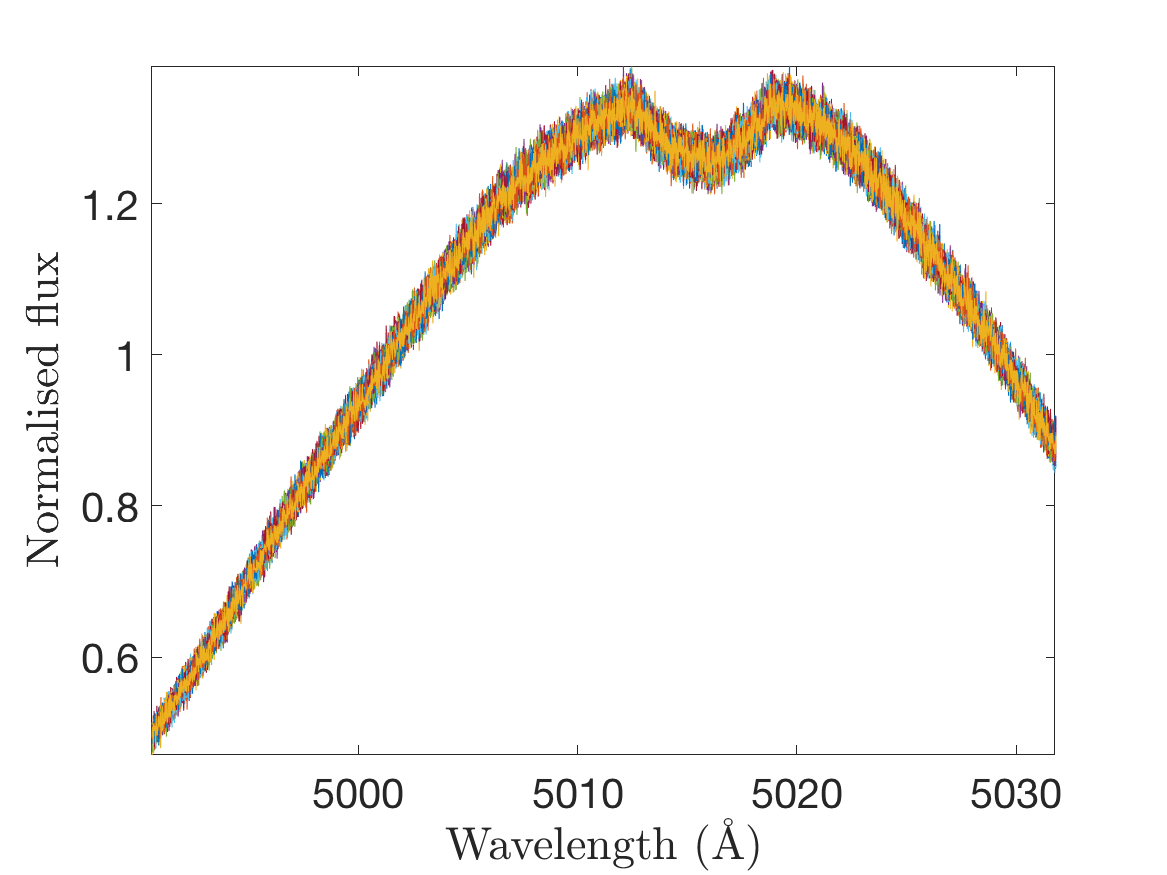
\includegraphics[width=0.8\textwidth]{HD148605_broad_lines.png}}\\
    \subfloat[ISV plot for HD148605.]{\label{figHD148605_ISV}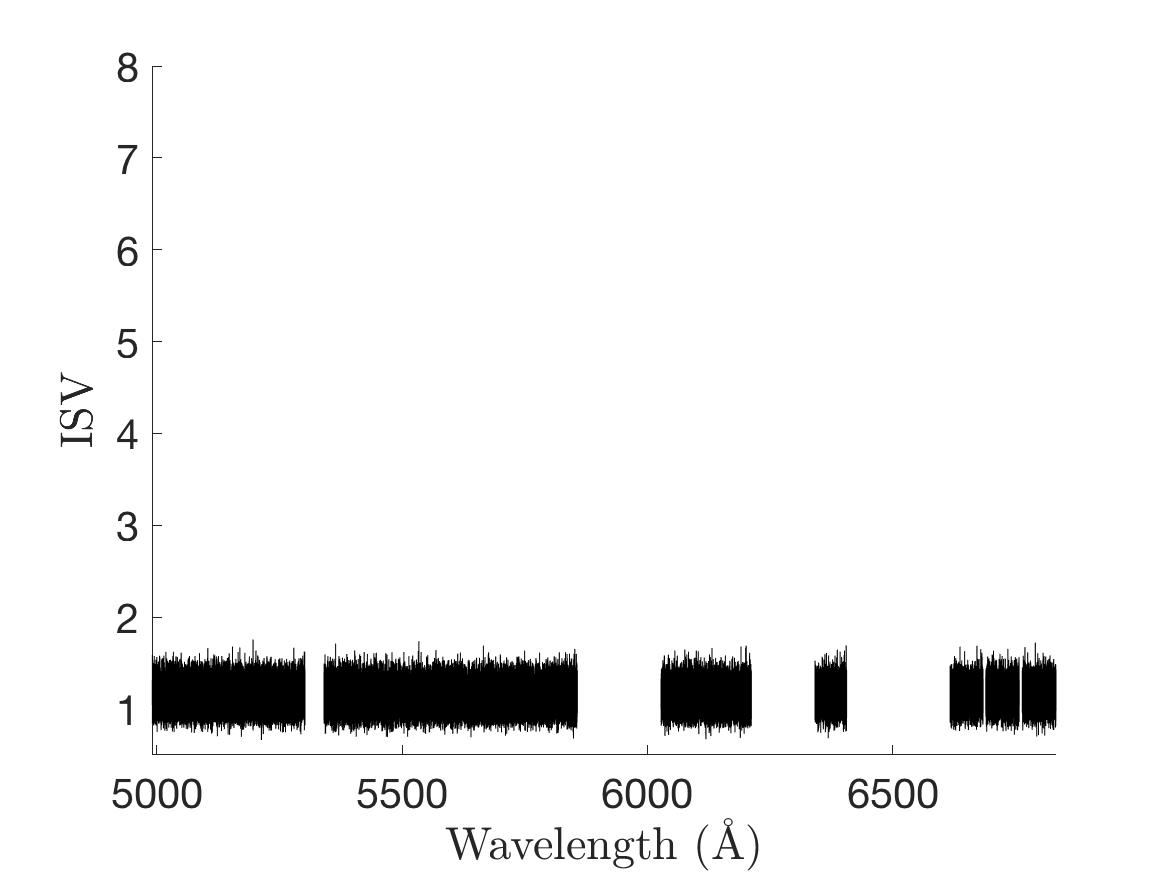
\includegraphics[width=0.8\textwidth]{HD148605_comparison.png}}
    \caption{}
    \label{figHD146805}
\end{figure}

To examine the impact of sky emission lines, a list of wavelengths, intensities, and FWHM of sky lines produced using the UV-visual Echelle Spectrograph (UVES; \citealt{1992Dekker}) were compared to the ISV lines in the M-dwarf sample. The only night sky emission lines seen to correspond to significant ISV features are the O\textsc{I} lines at 5577.3467\,\hbox{\AA} and 6363.7827\,\hbox{\AA}, with ISV lines at both wavelengths which can be seen in the ISV spectrum of GL514 (Figure\,\ref{figGL514sky}). To ensure that sky emission lines do not appear as false ISV signals in the analysis, the wavelengths of these two lines were masked in all spectra prior to barycentric and radial velocity correction, and the ISV calculations were run again. To ensure that the entire line was removed, all wavelengths within two FWHM on either side of the central wavelength of both sky lines were masked.  Figure\,\ref{figGL514nosky} shows the ISV spectrum for GL514 once the sky lines had been removed. The remaining sky lines did not produce ISV signatures significantly above the baseline noise at the wavelengths used. A check for, and subsequent masking of, any visible sky emission lines will be required for spectra using wavelengths other than the ones used in this work.\\

\begin{figure}
    \centering
	\captionsetup{width=.8\textwidth}
    \subfloat[An ISV plot for GL514. Sky emission is responsible for the ISV lines at $\sim$5577\,\hbox{\AA} and $\sim$6364\,\hbox{\AA}.]{\label{figGL514sky}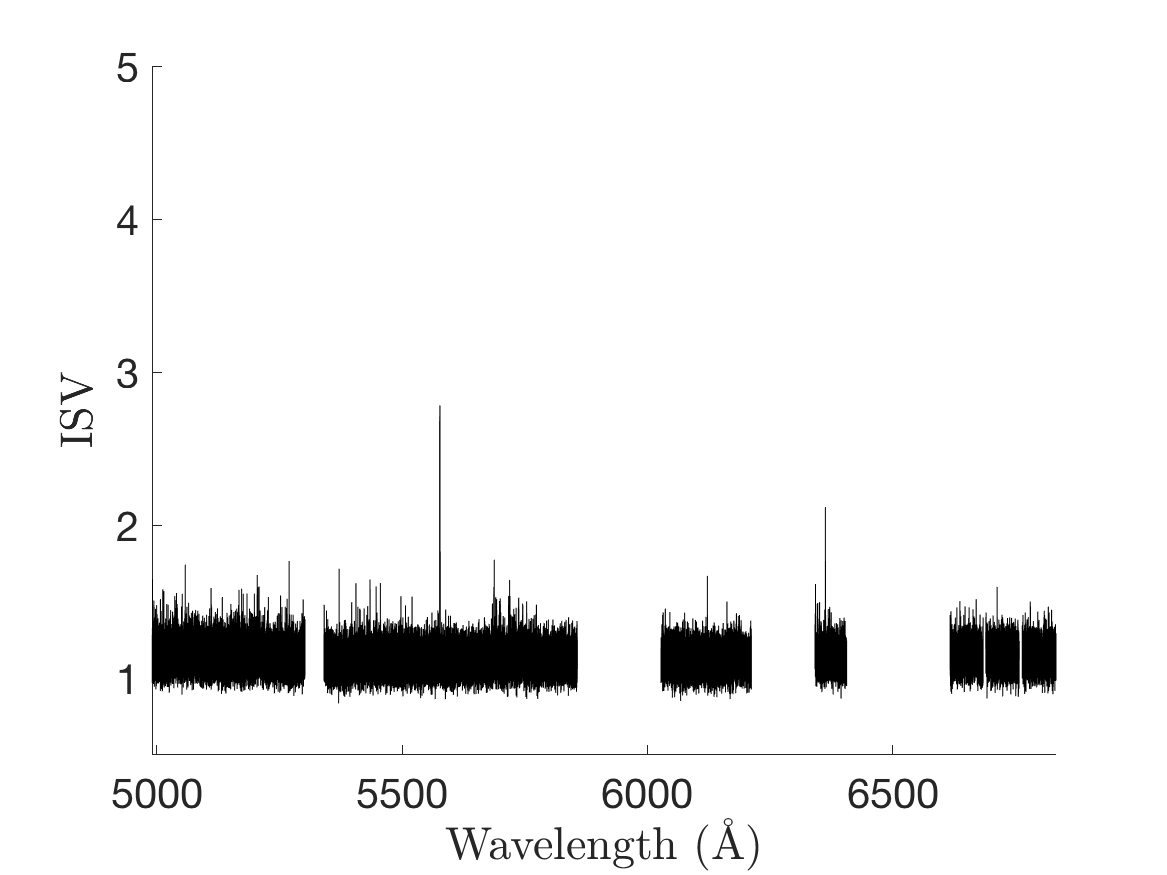
\includegraphics[width=0.8\textwidth]{Gl514_sky.png}}\\
    \subfloat[The ISV plot for GL514 once the suspected sky lines have been masked.]{\label{figGL514nosky}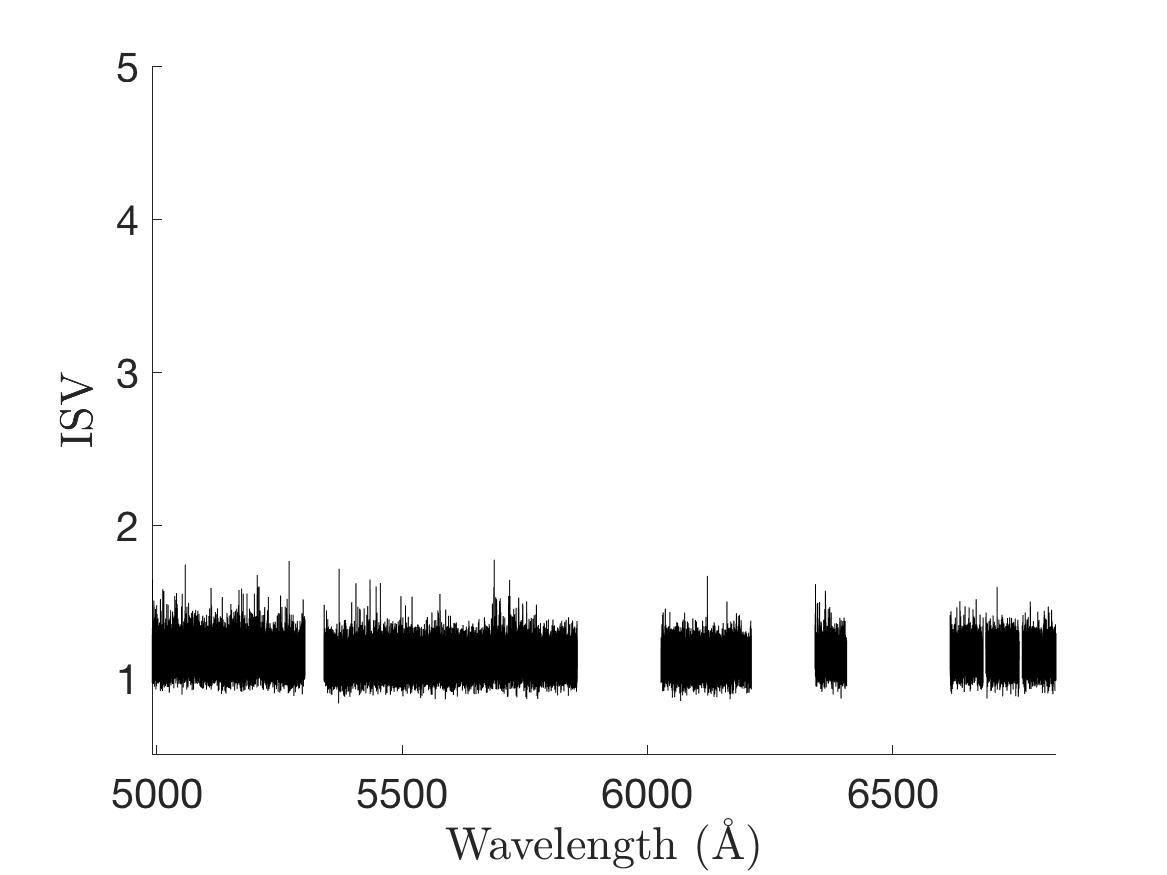
\includegraphics[width=0.8\textwidth]{Gl514_no_sky.png}}
    \caption{}
    \label{figGL514}
\end{figure}

\subsection{Wavelengths exhibiting significant ISV peaks}
\label{secISVlines}
To identify wavelengths with features significantly higher in ISV than the baseline noise, a selection threshold is required. Assuming the distribution function of the ISV spectrum is Gaussian, setting a threshold at the 99.7 percentile (equivalent to 3$\sigma$) of the ISV for a star should confidently separate significant ISV lines from the baseline noise. Figure\,\ref{figThreshold} shows a histogram of the ISV spectrum for GL87.\\

\begin{figure}[!h]
    \centering
	\captionsetup{width=.8\textwidth}
    \subfloat[A histogram of the ISV values for GL87. The 99.7th percentile separates the brown and blue regions. The plot has been zoomed in to highlight the data above and below the 99.7th percentile.]{\label{figGL87_hist}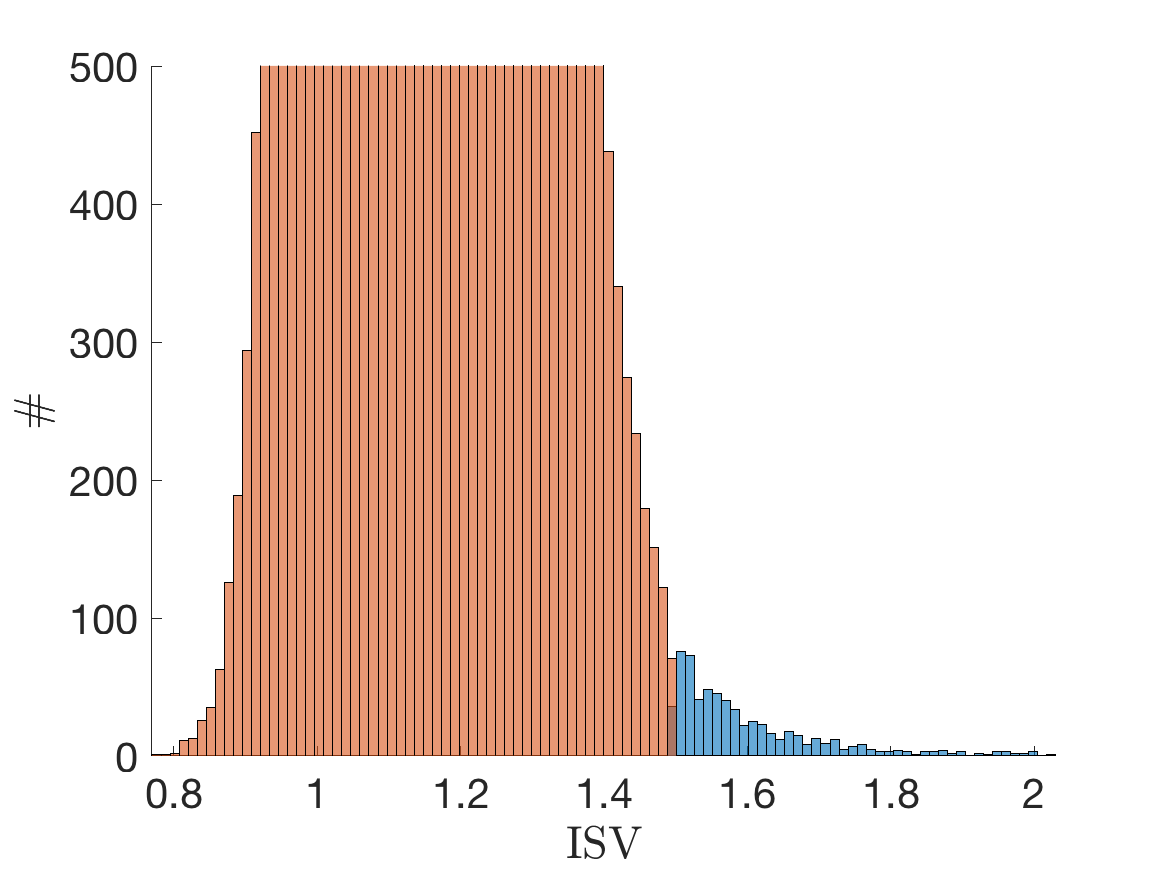
\includegraphics[width=0.8\textwidth]{Gl87_threshold_hist.png}}\\
    \subfloat[ISV for GL87, with the red dashed line indicating the 99.7th percentile level.]{\label{figGL87_ISV}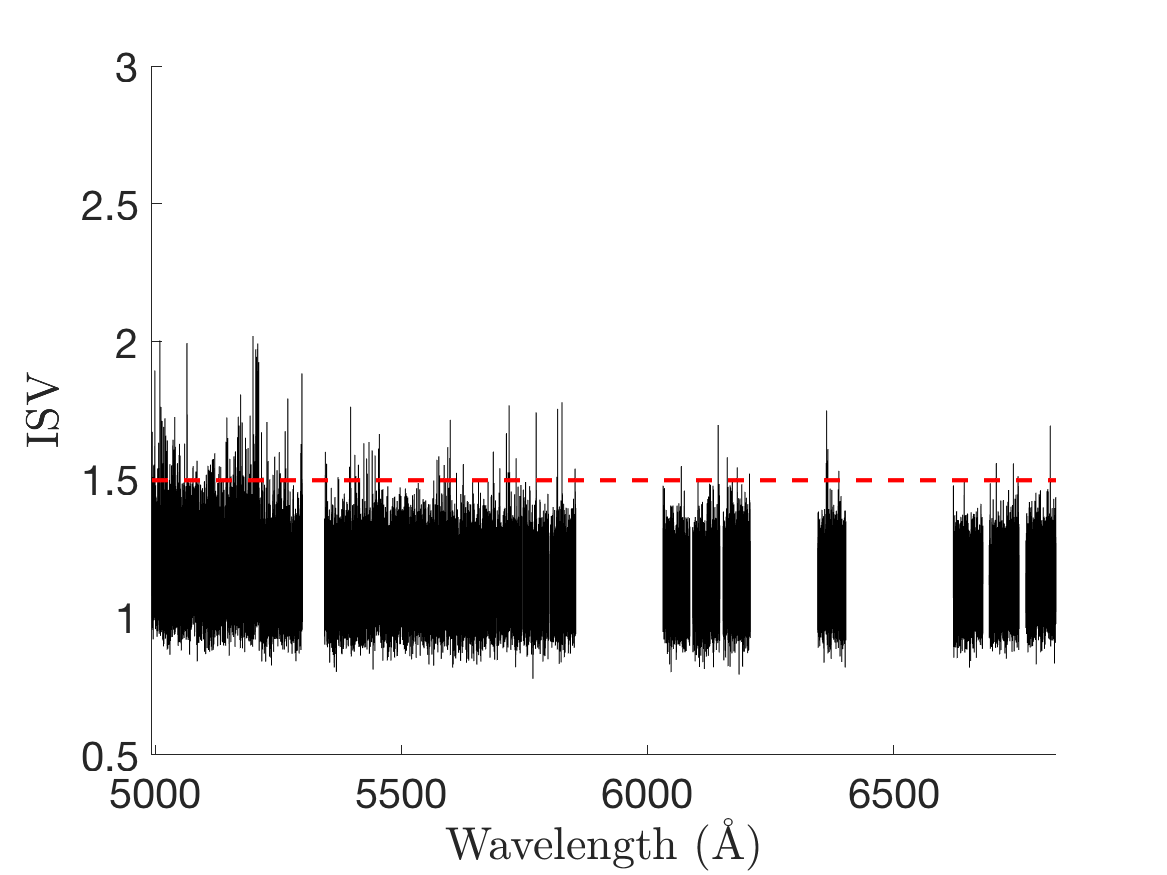
\includegraphics[width=0.8\textwidth]{Gl87_threshold_ISV.png}}
    \caption{}
    \label{figThreshold}
\end{figure}

For the bright stars with a flat baseline noise, this method suitably identifies a single threshold between the baseline noise and ISV lines. For dimmer stars, the baseline noise is less flat, and a single threshold based on the ISV distribution will be problematic. Figure\,\ref{figGL551_bad_threshold} shows an extreme example of this for the star GL551. It is clear that determining the threshold from the 99.7th percentile in a star with a non-flat baseline noise will result in a threshold so high that multiple lines at longer wavelengths would be excluded. As the non-flat regions appeared predominantly in the first 8 orders, the solution was to exclude those orders from the percentile calculation. Compared to Figure\,\ref{figGL551_bad_threshold}, the threshold for GL551 in Figure\,\ref{figGL551_good_threshold} is more representative of the entire wavelength range. For stars with a flat baseline noise, excluding the first 8 orders did not change the threshold by a significant amount. For stars with a non-flat baseline noise, excluding the first 8 orders reduced their influence on the determination of the threshold, ensuring that ISV lines from the redder wavelengths were not excluded. However, a consequence of lowering the threshold was that regions of baseline noise in the non-flat orders would extend above that threshold, complicating analysis of ISV lines at those wavelengths. The methodology for selecting and identifying individual ISV lines needed to account for this and is discussed in the next section. The ISV spectrum for each star in the M-dwarf sample is presented in Section\,\ref{secResults}, where the red dashed line is the 99.7th percentile threshold.\\

\begin{figure}[!h]
    \centering
	\captionsetup{width=.8\textwidth}
    \subfloat[Due to the structure present in the ISV of GL551, the baseline noise varies strongly from order to order, lifting the 99.7th percentile to a much higher ISV level.]{\label{figGL551_bad_threshold}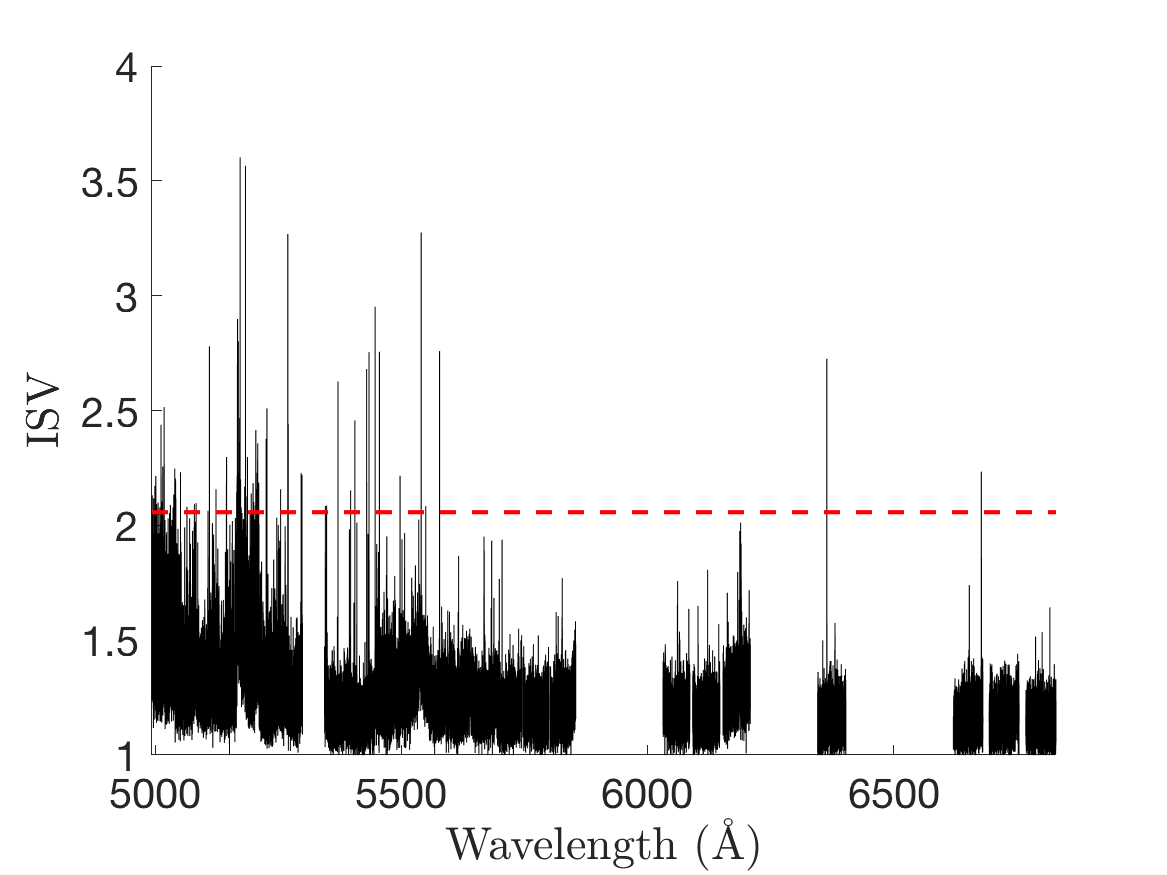
\includegraphics[width=0.8\textwidth]{GL551_baseline.png}}\\
    \subfloat[The 99.7th percentile threshold level for GL551 if the non-flat orders are excluded.]{\label{figGL551_good_threshold}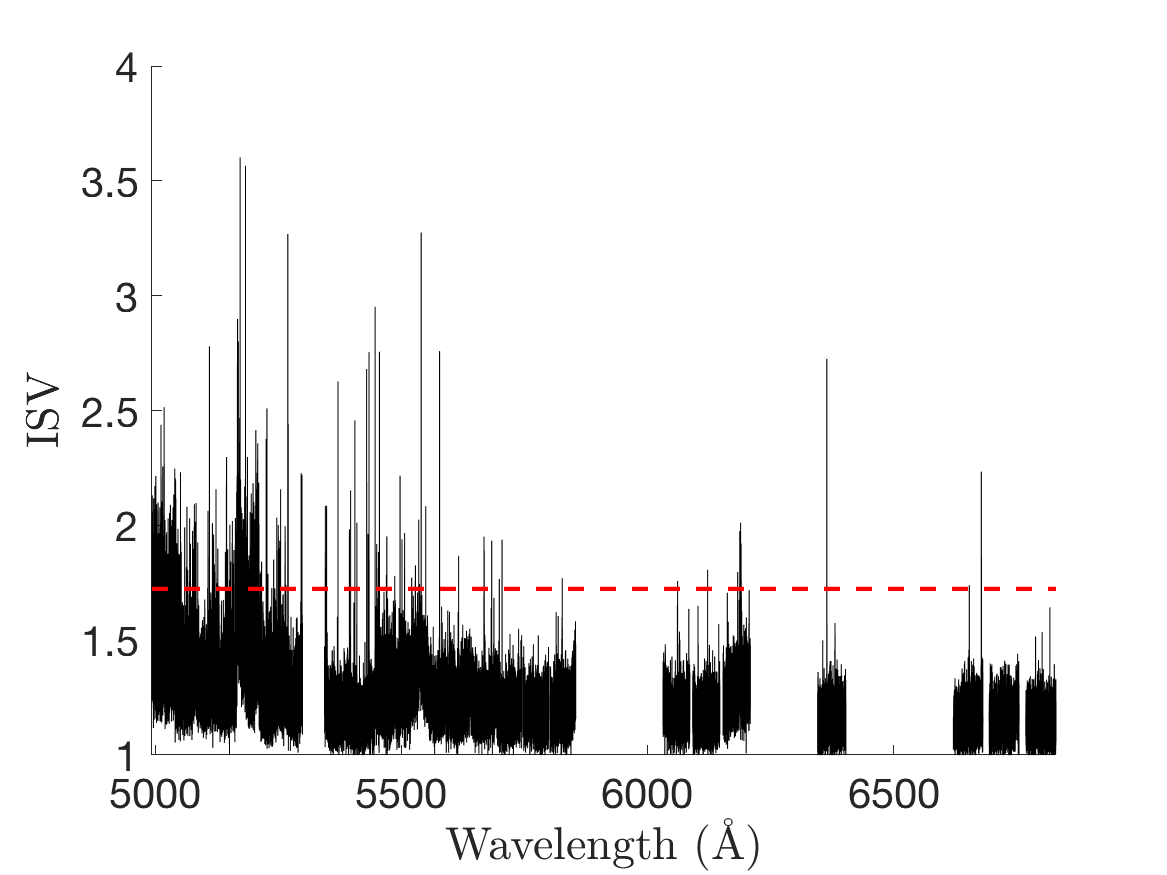
\includegraphics[width=0.8\textwidth]{Gl551_ISV_with_threshold.png}}
    \caption{}
    \label{figBaseline}
\end{figure}

Wavelengths with an ISV value above the threshold should generally correspond to individual varying spectral lines; however, not all may really be spectral lines. There there may be some artifacts produced by the reduction or cosmic rays that manage to pass the sigma-clipping step and produce a false-positive ISV signal. One way to exclude these false-positives is to require them to have a FWHM broader than the spectrograph resolution. Even if an ISV line happened to fall at the same wavelength as a real spectral line, if it was too narrow to resolve, it could not actually be due to spectral line variability. Those ISV lines that pass this width criterion were then compared with known atomic line features using a line list compiled by the GALAH survey \citep{2018Buder}. The line list was compiled from spectral lines frequently seen in solar-type stars. This is an advantage and a disadvantage as ISV lines can be confidently identified if they have the same wavelength as a spectral line in the list, but as the spectra of G- and M-dwarfs will differ, there will be a number of unidentified ISV lines. Developing a robust M-dwarf line list is a complex task due to the number of molecular bands that develop in late M-dwarf spectra. The GALAH line list, while sub optimal for M-dwarfs, is still reasonable as it is used as a tool to assist in the development of the ISV metric, and is not the central focus of this work. Details of the line list are presented in Table\,\ref{tabLineList}. A non-linear, least-squares fitting routine, inbuilt into MATLAB\footnote{The Math Works, Inc. MATLAB, version 2017b. https://www.mathworks.com/}, was used to fit a Gaussian to each ISV line above the threshold. The central wavelength of the Gaussian was adopted as the wavelength of the ISV line, and the HWHM of the Gaussian was adopted as the uncertainty on the fitted wavelength of the ISV line. An ISV line was confirmed to be an ISV spectral line if a spectral line from Table\,\ref{tabLineList} fell within that HWHM uncertainty from the Gaussian centroid (e.g. within the red dashed lines in Figures\,\ref{figLine3} and \ref{figLine4}). Figure\,\ref{figGL551_Element} provides examples of the quantities measured to determine the strength of an ISV line. The signal-to-noise of an ISV line will have a strong influence on the the quality and measurement of the line. Figure\,\ref{figLine1} displays an ISV line from a Fe\,\textsc{i} line transition at $\lambda\,=\,5429.6964\hbox{\AA}$. This line is strong when compared to the noise around it and has a clear Gaussian-like shape. Figure\,\ref{figLine2} is an example of a lower quality ISV line produced by a Cr\,\textsc{i} transition at $\lambda\,=\,5206.023\hbox{\AA}$. The magnitude of the line is still significant, albeit weaker than the Fe\,\textsc{i} line in Figure\,\ref{figLine1}. However, the relatively strong baseline noise interferes with the wings of the ISV line and makes it harder to accurately fit a Gaussian to the ISV line.\\

\begin{figure}[!h]
	\captionsetup{width=.8\textwidth}
    \subfloat[Fe\,\textsc{i}]{\label{figLine1}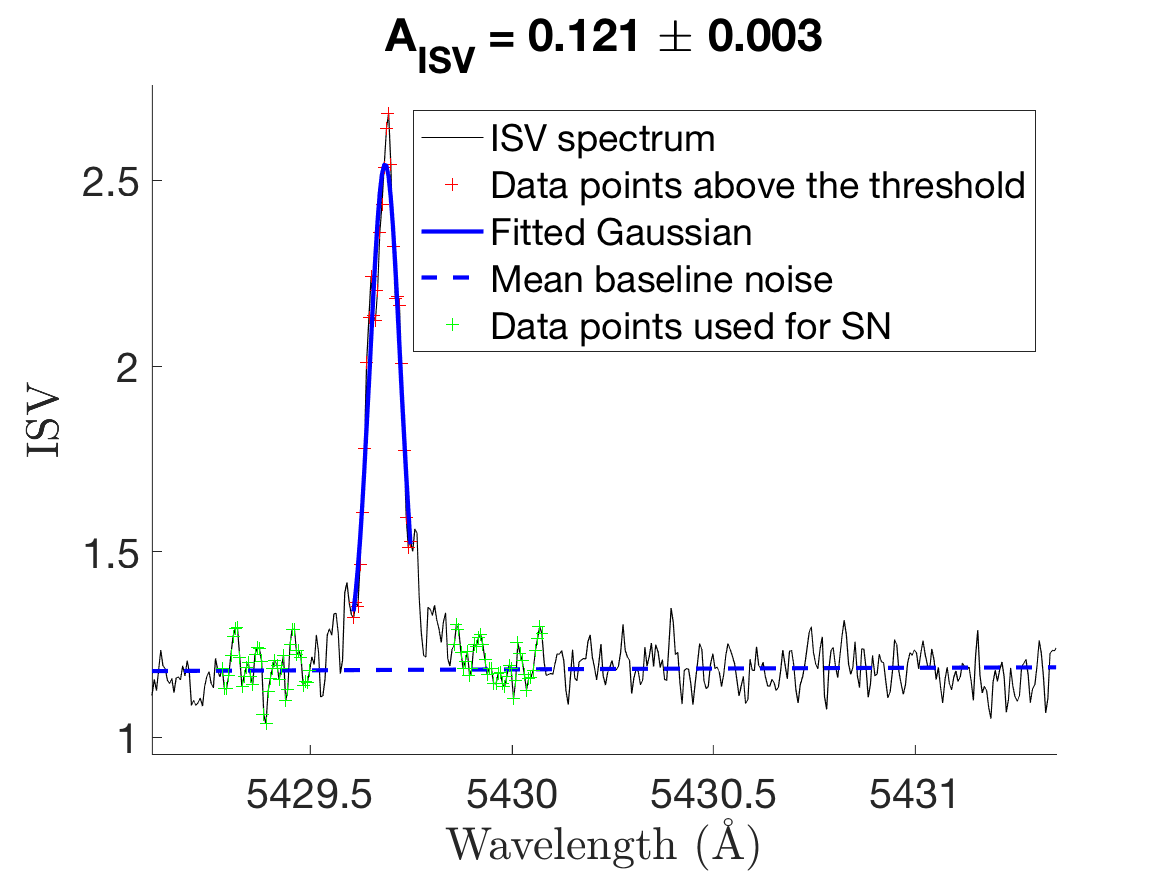
\includegraphics[width=0.5\textwidth]{Gl551_ISV_value.png}}
    \subfloat[Cr\,\textsc{i}]{\label{figLine2}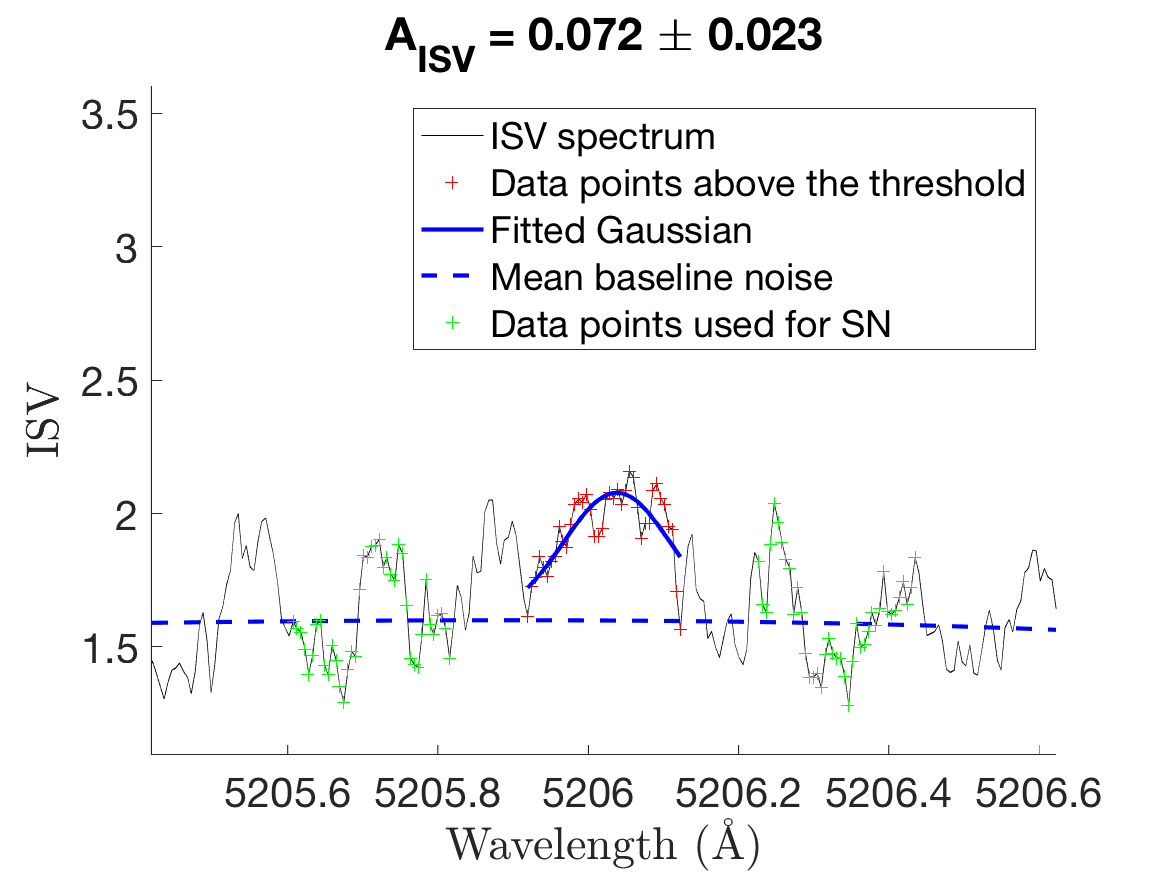
\includegraphics[width=0.5\textwidth]{Gl551_ISV_value2.png}}\\
    \subfloat[Fe\,\textsc{i}]{\label{figLine3}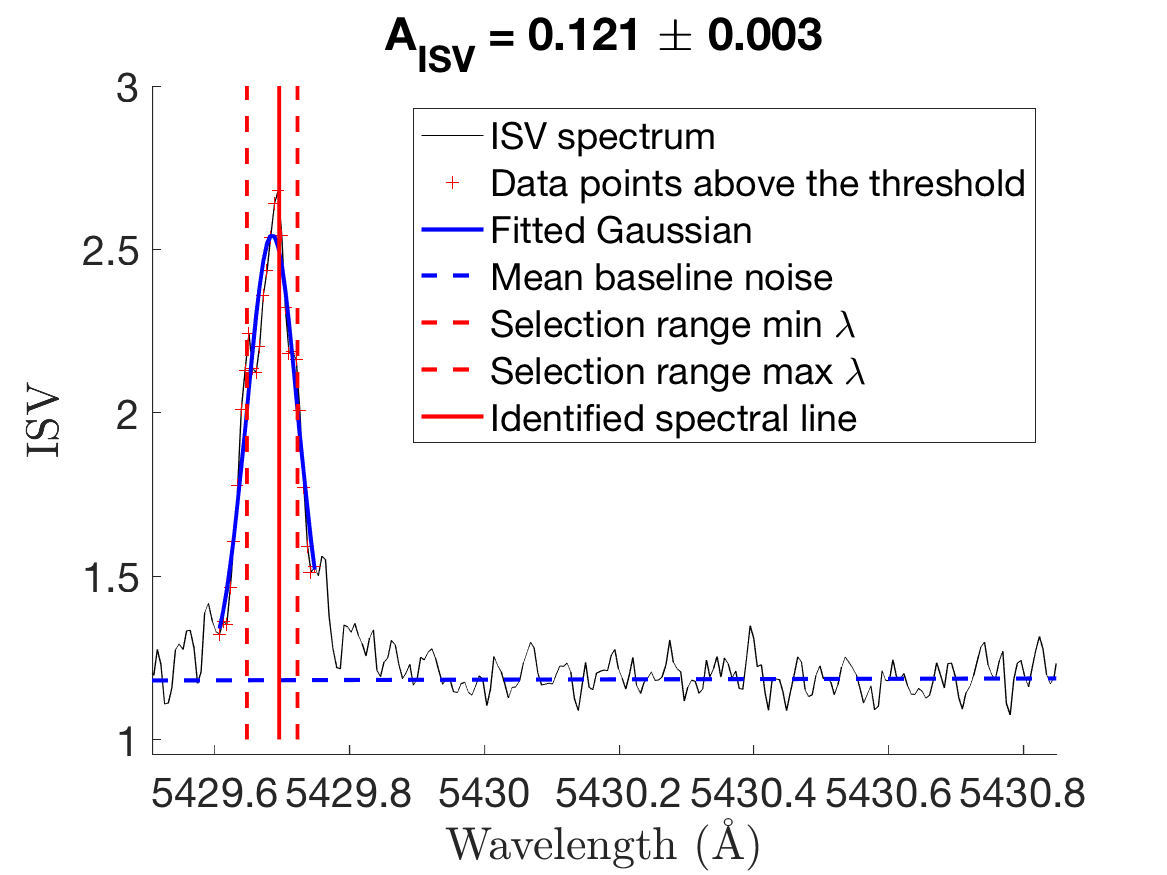
\includegraphics[width=0.5\textwidth]{Gl551_ISV_value_zoom.png}}
    \subfloat[Cr\,\textsc{i}]{\label{figLine4}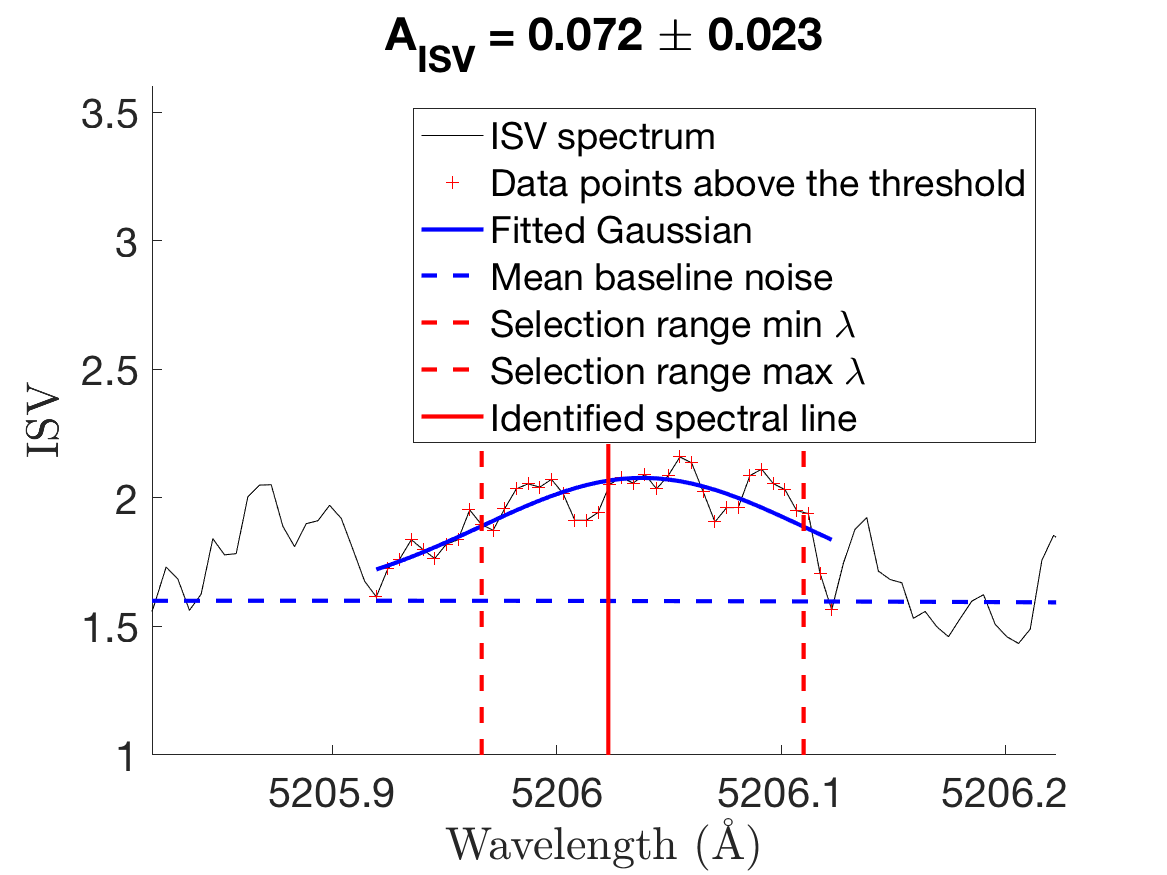
\includegraphics[width=0.5\textwidth]{Gl551_ISV_value2_zoom.png}}\\
    \caption{Two ISV lines from GL551, one clearly identifiable above the baseline noise, and another that is less prominent and in a 'noisier' region. The red points were used for calculating the strength of the feature, and the blue solid line is the Gaussian fitted to the red points to determine the centroid. The blue dashed line represents the mean baseline noise, and the green points were used to determine the signal-to-noise of the mean baseline noise around the ISV feature. The bottom plots are zoomed-in copies of the top plots. The solid red vertical line indicate the rest wavelength of the identified spectral line, and the dashed red vertical lines represent the wavelength range on either side of the Gaussian centroid where a spectral line from the line list needs to fall into to confirm which spectral line correlates with the ISV line.}
    \label{figGL551_Element}
\end{figure}

Once the ISV spectral line is identified, its strength can be quantified by integrating the area between the ISV and the mean baseline noise. The boundary between the baseline noise and the ISV spectral line was determined as the 95th percentile (2\,$\sigma$) of the ISV across the full wavelength range of the order. The ISV spectral line, ISV($\lambda$), was then the points above this threshold. To determine the mean of the baseline noise, the ISV of each order was sigma-clipped to remove all points more than 3$\sigma$ from the mean, and a 10th order polynomial was fitted to represent the mean baseline noise for that order (B($\lambda$)). This is shown as blue dashed lines in Figure\,\ref{figGL551_Element}. A 10th order polynomial was required to ensure that the shape of the baseline noise was properly measured in both flat and non-flat regions. Lower order polynomials and splines were investigated and were found not to reliably estimate the mean baseline noise. The lower order polynomials were suitable for orders that were `flat’, but they  tended to ignore the changes in the baseline found in the `non-flat’ orders. Splines would often provide a suitable mean baseline, but for a number of stars they would fail to fit to the start and end points of the data. A 10th order polynomial was the lowest order to fit to the data properly for all stars in the sample. The mean baseline noise was then subtracted from the ISV spectral line to obtain the magnitude of the spectral line variation above the baseline noise. Summing these values over the pixels selected and multiplying by the average wavelength dispersion, $\Delta\lambda$, gave the ISV spectral line strength, $A_{ISV}$ (Equation\,\ref{eqA_ISV}) with units of \hbox{\AA}. $A_{ISV}$ is therefore effectively a ``variability equivalent width''.\\

The uncertainty in $A_{ISV}$ was obtained by adapting a method for obtaining the uncertainty in equivalent widths (\citealt{1995Ebbets}; Equation\,\ref{eqd_A_ISV}). To estimate the signal-to-noise (S/N), the standard deviation of 40 points either side of the ISV spectral line was determined, and the mean of these two values was used. The 40 pixels correspond to a wavelength range of 0.23\hbox{\AA}, comparable to the wavelength range of the ISV line. These are the green points in Figure\,\ref{figGL551_Element}. The signal-to-noise was then the mean value of the ISV across the data points divided by the noise (Equation\,\ref{eqSN}).\\

%\begin{equation}
%    A_{ISV} = \sum\limits_{i=1}^n (ISV(\lambda)-B(\lambda)) \Delta\lambda
%    \label{eqA_ISV}
%\end{equation}

%\begin{equation}
%    \Delta A_{ISV} = \frac{\sqrt{\sum\limits_{i=1}^n\frac{n\Delta\lambda^2 ISV(\lambda)}{S/N(\lambda)^2}}}{n}
%    \label{eqd_A_ISV}
%\end{equation}

%\begin{equation}
%    SN(\lambda) = \frac{\sum\limits_{i=1}^n ISV(\lambda)-B(\lambda)}{nN}
%    \label{eqSN}
%\end{equation}

\begin{table}[]
    \centering
    \begin{tabular}{|c|}
    \hline
    \vbox{\begin{equation}A_{ISV} = \sum\limits_{i=1}^n (ISV(\lambda)-B(\lambda)) \Delta\lambda\label{eqA_ISV}\end{equation}}\\
    \vbox{\begin{equation}\Delta A_{ISV} = \frac{\sqrt{\sum\limits_{i=1}^n\frac{n\Delta\lambda^2 ISV(\lambda)}{S/N(\lambda)^2}}}{n}\label{eqd_A_ISV}\end{equation}}\\
    \vbox{\begin{equation}SN(\lambda) = \frac{\sum\limits_{i=1}^n ISV(\lambda)-B(\lambda)}{nN}\label{eqSN}\end{equation}}\\
    \hline
    \end{tabular}
    \caption{Equations used to measure the magnitude of ISV variability in an ISV spectrum.}
    \label{tabISVaisv}
\end{table}
Comparing the `strong' and `weak' example ISV lines of Figures\,\ref{figLine1} and \ref{figLine2}, the $A_{ISV}$ magnitude (displayed above each plot) is stronger for the Fe\,\textsc{i} line than for the Cr\,\textsc{i} line and the uncertainty of the Cr\,\textsc{i} line is greater than for the Fe\,\textsc{i} line. However more significantly, due to the stronger baseline noise, the uncertainty of the Cr\,\textsc{i} line is 33\% the magnitude of the $A_{ISV}$, while for the Fe\,\textsc{i} it is only 4\%.

\subsection{ISV and canonical stellar activity indices}
\label{secOtherInd}
As discussed in Section\,\ref{secVarQuant}, line strength indices for Ca H\&K, H$\alpha$, and Na D are well studied proxies for chromospheric activity in stars. Analysis of how correlated the $A_{ISV}$ is to the S-indices could provide a better understanding of what types of activity $A_{ISV}$ is sensitive to. The S-indices for Ca\,\textsc{ii} H \& K, H\,\textsc{$\alpha$}, and Na\,\textsc{i} D, with their respective instrumental uncertainties, were measured for all of the stars using the methodology described in \citet{2011Gomes} to provide a known measure of variability for comparison with $A_{ISV}$. Also mentioned in Section\,\ref{secVarQuant} was that the Ca H\&K S-index was not as useful for cool stars as the other two indices. However the ISV metric was designed to be suitable for all classes of star, and some knowledge of how $A_{ISV}$ correlates with $S_{HK}$ will still be beneficial. Therefore the Ca H\&K S-index was included alongside H$\alpha$, and Na D for the sake of completeness. The S-index provides a value for each observation while $A_{ISV}$ is a single measurement for each star, making it difficult to directly compare them. The solution was to compare $A_{ISV}$ with the median S-index value across all observations of a star. For the uncertainty of this median S-index, Equation\,\ref{eqSerr} was used, where $N$ is the number of observations, $\Delta S_{mean}$ is the uncertainty in the mean, given by Equation\,\ref{eqSmean}, $\sigma_{S}$ is the RMS of the S-index values across all observations of a star, and $n = \frac{N-1}{2}$. The resulting median S-indices for each star are presented in Table\,\ref{tabHARPSactive}.\\

\begin{equation}
    \Delta S_{med} = \Delta S_{mean}\sqrt{\frac{\pi(2n+1)}{4n}}
    \label{eqSerr}
\end{equation}

\begin{equation}
    \Delta S_{mean} = \frac{\sigma_{S}}{\sqrt{N}}
    \label{eqSmean}
\end{equation}

Figures\,\ref{figCaHK}, \ref{figHalpha}, and \ref{figNaD} show the resulting median S-indices. The stars have been ordered into ascending Ca\,\textsc{ii} H \& K values and divided into two groups. The Ca\,\textsc{ii} H \& K S-index values do not change significantly from GJ2066 to GL701, and rise rapidly starting from GL752A. Based on this behaviour the stars were divided into a `quiescent' subsample (S$_{CaHK}$\,\textless\,0.1, plotted as blue points) and an 'active' subsample (S$_{CaHK}$\,\textgreater\,0.1, plotted as red points). A visual comparison of Figures~\ref{figHalpha}, and \ref{figNaD} indicate that the grouping of quiescent and active stars for S$_{CaHK}$ also applies for S$_{Ha}$, and may apply for S$_{NaD}$ (albeit weakly). This consistency of this grouping across these activity metrics is supported by the Pearson correlation coefficients between each of the indices. Ca\,\textsc{ii} H \& K had a 0.905 correlation with H\,\textsc{$\alpha$}, and a 0.724 correlation with Na\,\textsc{i} D. H\,\textsc{$\alpha$} and Na\,\textsc{i} D have a 0.570 correlation between them. This suggests that Ca\,\textsc{ii} H \& K and H\,\textsc{$\alpha$} are reacting to stellar activity in the same way, while the behaviour of Na\,\textsc{i} D may have other influences. 

\begin{sidewaysfigure}
    \vspace{-1cm}
    \centering
    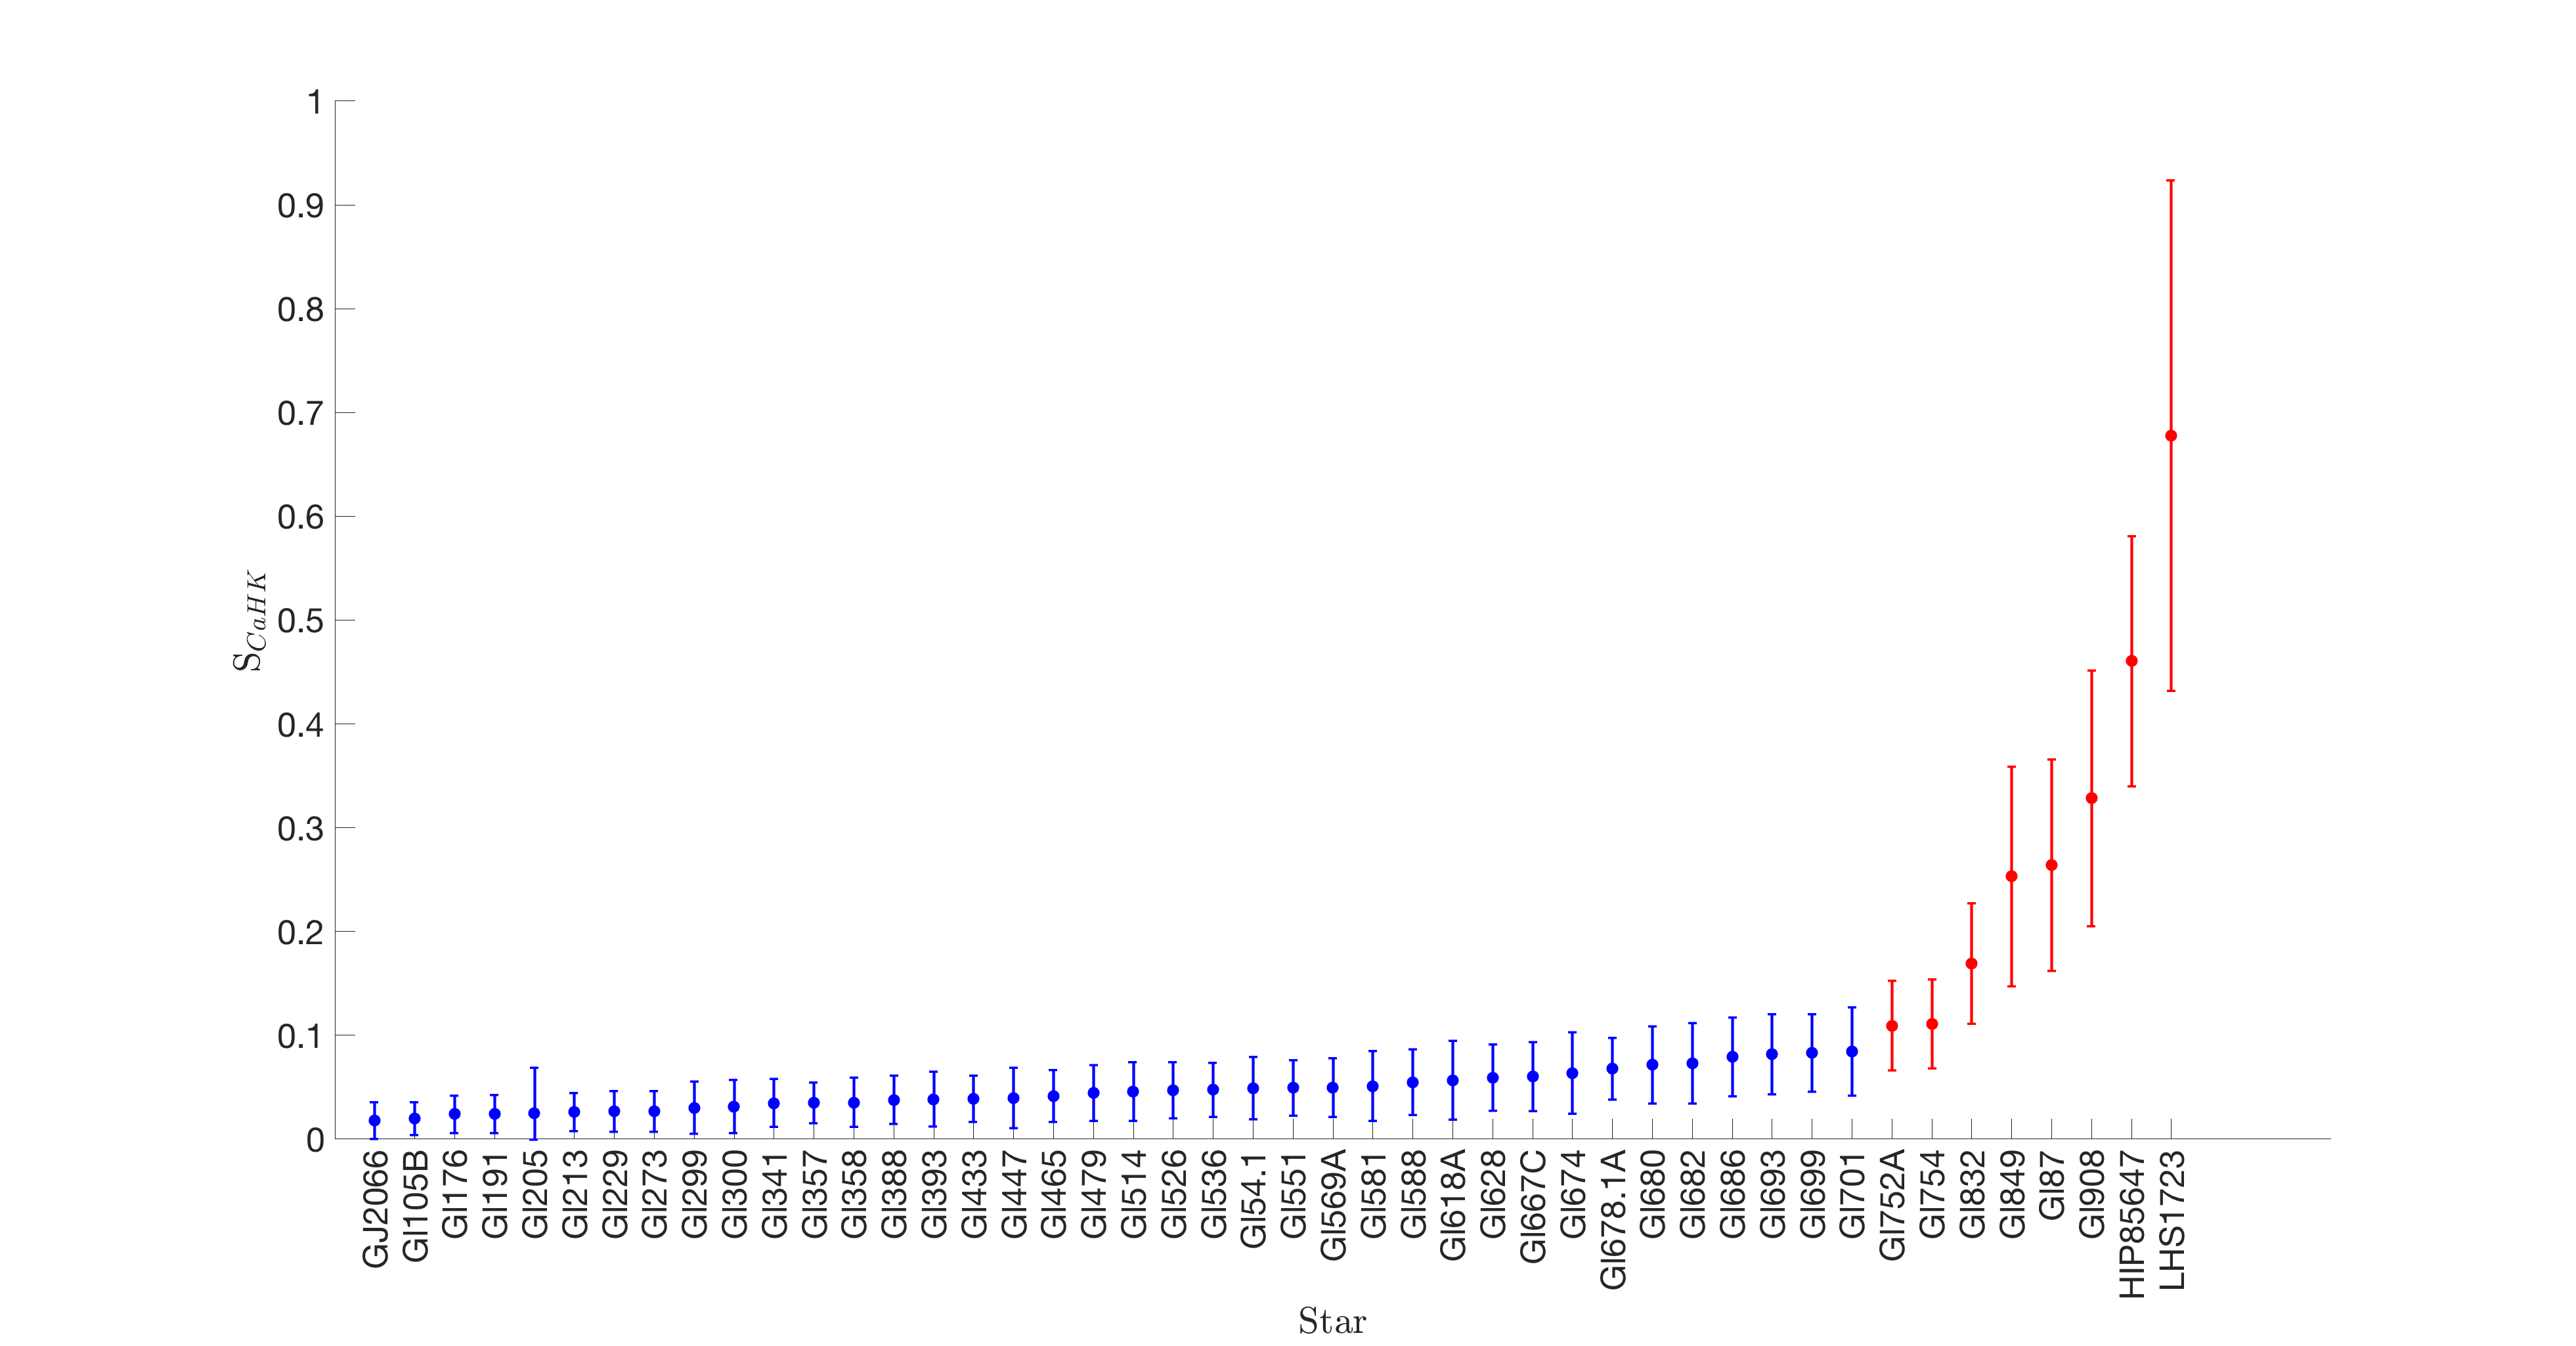
\includegraphics[width=\textwidth]{CaHK.png}
    \caption{Median index values for Ca\,\textsc{ii} H \& K for each of the N stars in the data set, arranged by ascending Ca H\&K S-index value.}
    \label{figCaHK}
\end{sidewaysfigure}
\begin{sidewaysfigure}
    \vspace{-1cm}
    \centering
    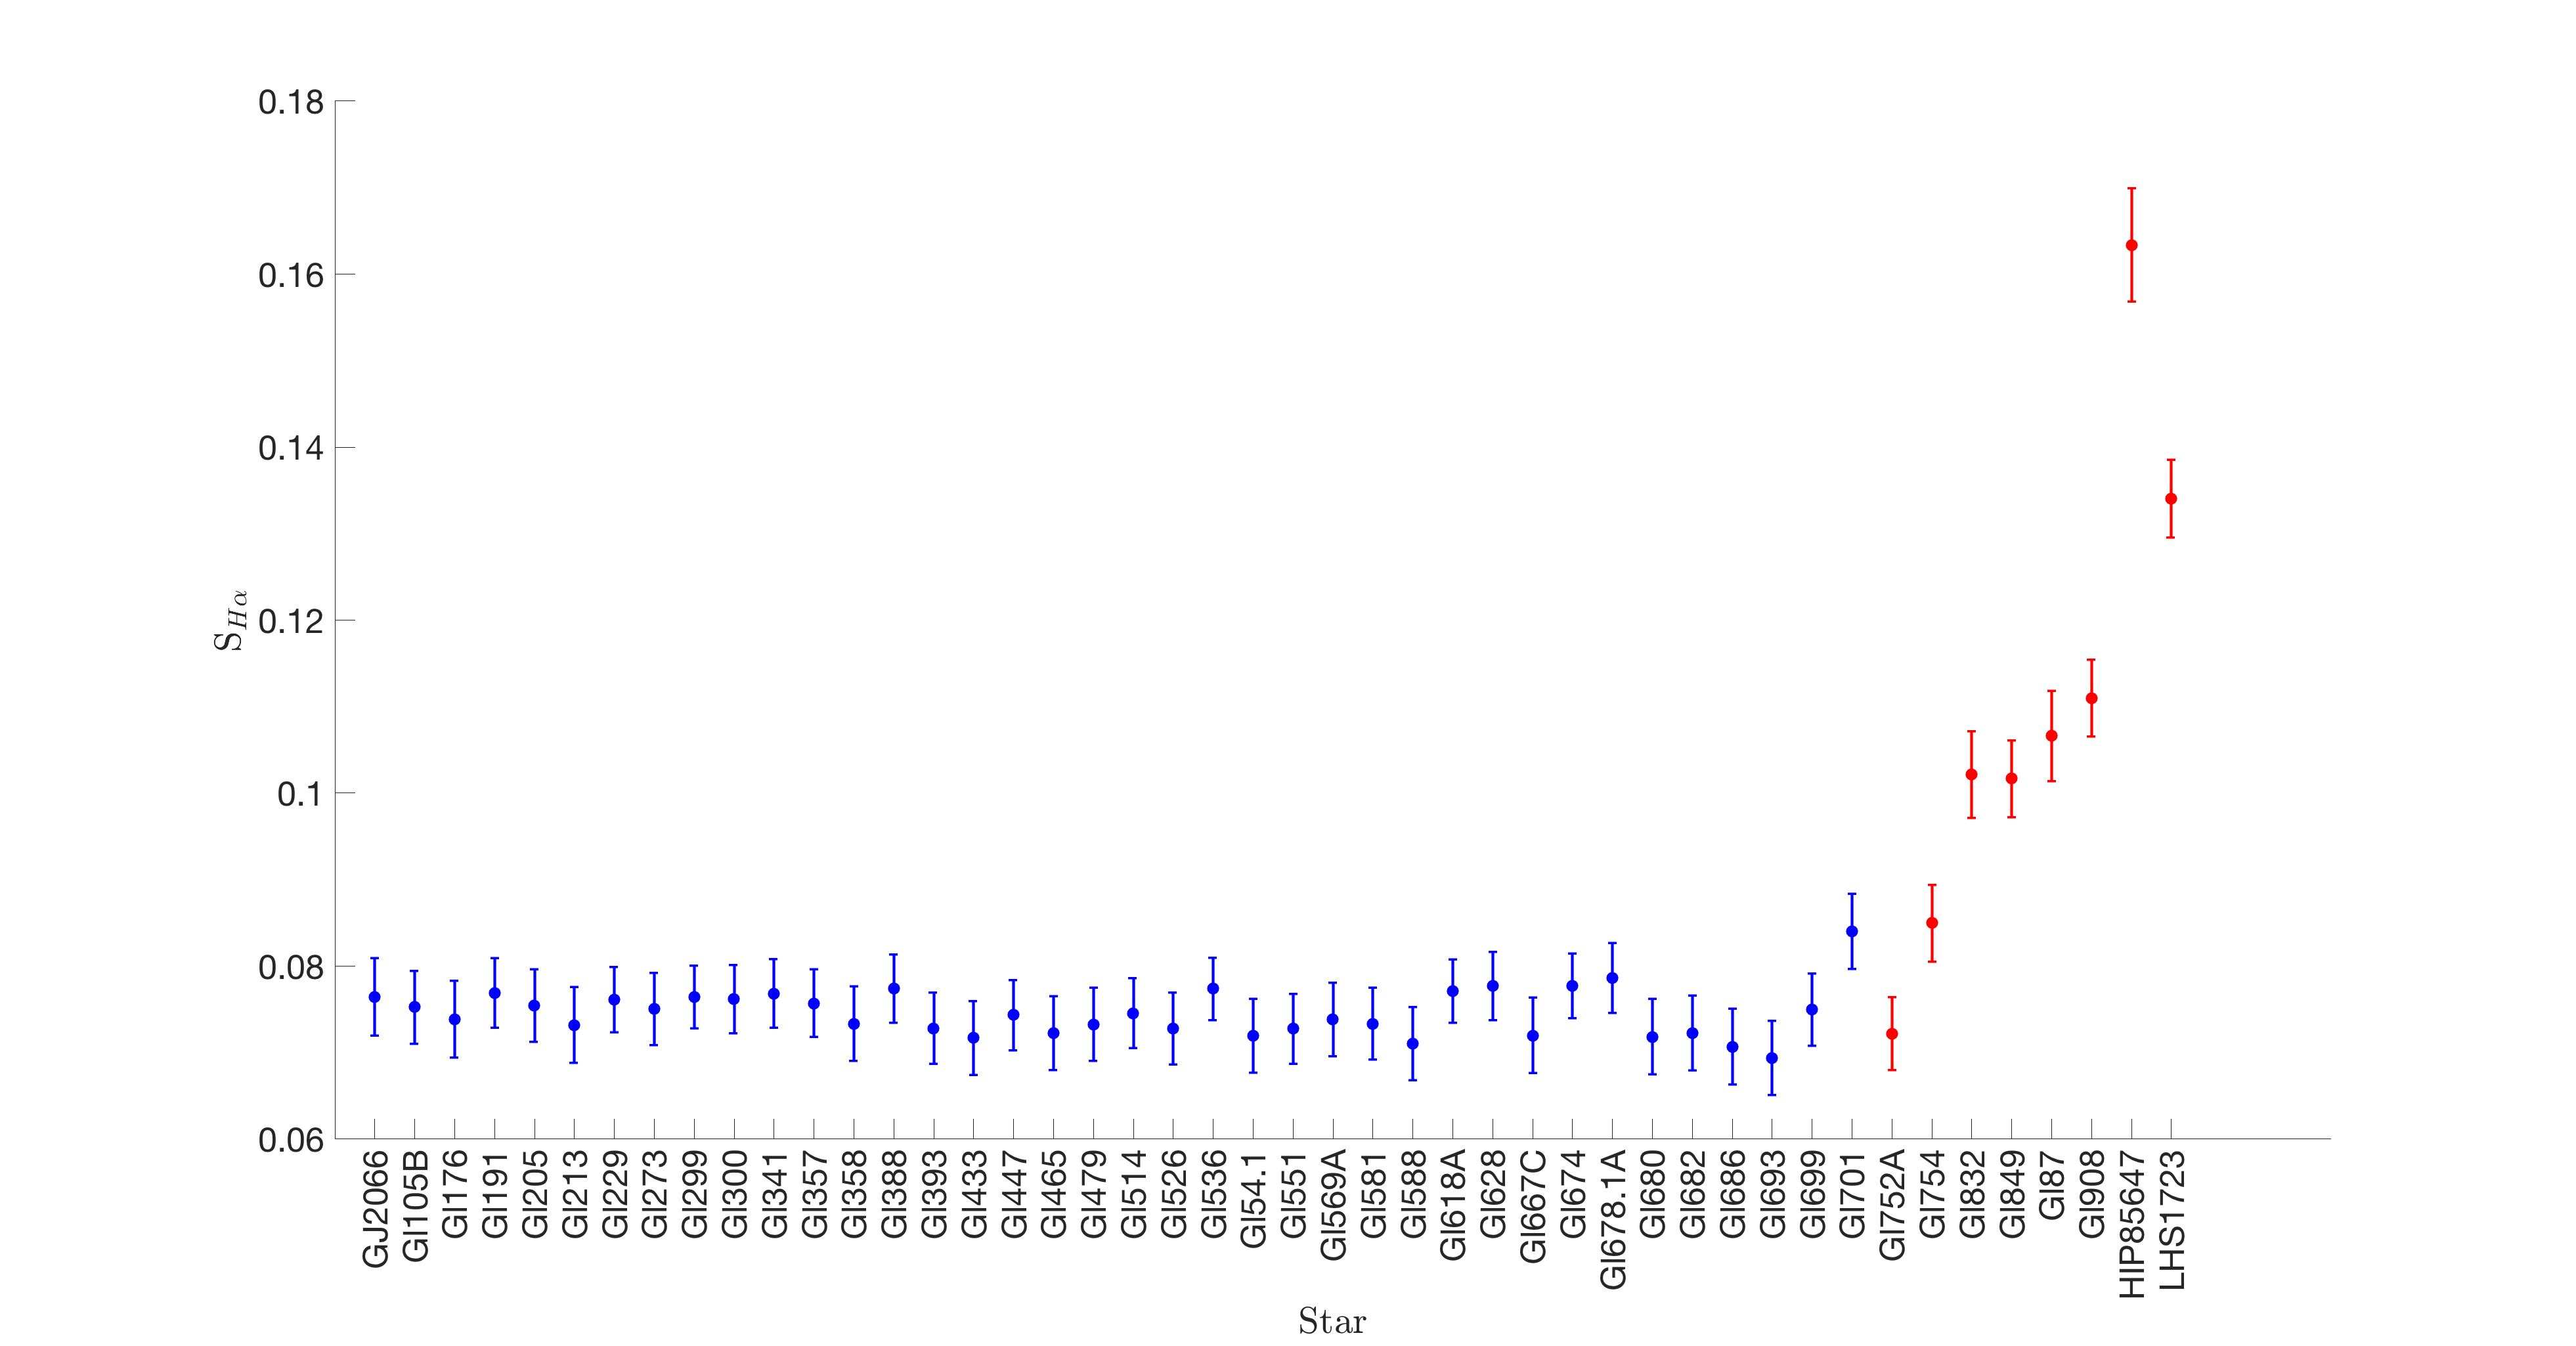
\includegraphics[width=\textwidth]{Halpha.png}
    \caption{Median index values for H\,\textsc{$\alpha$} for each of the N stars in the data set, arranged by ascending Ca H\&K S-index value.}
    \label{figHalpha}
\end{sidewaysfigure}
\begin{sidewaysfigure}
    \vspace{-1cm}
    \centering
    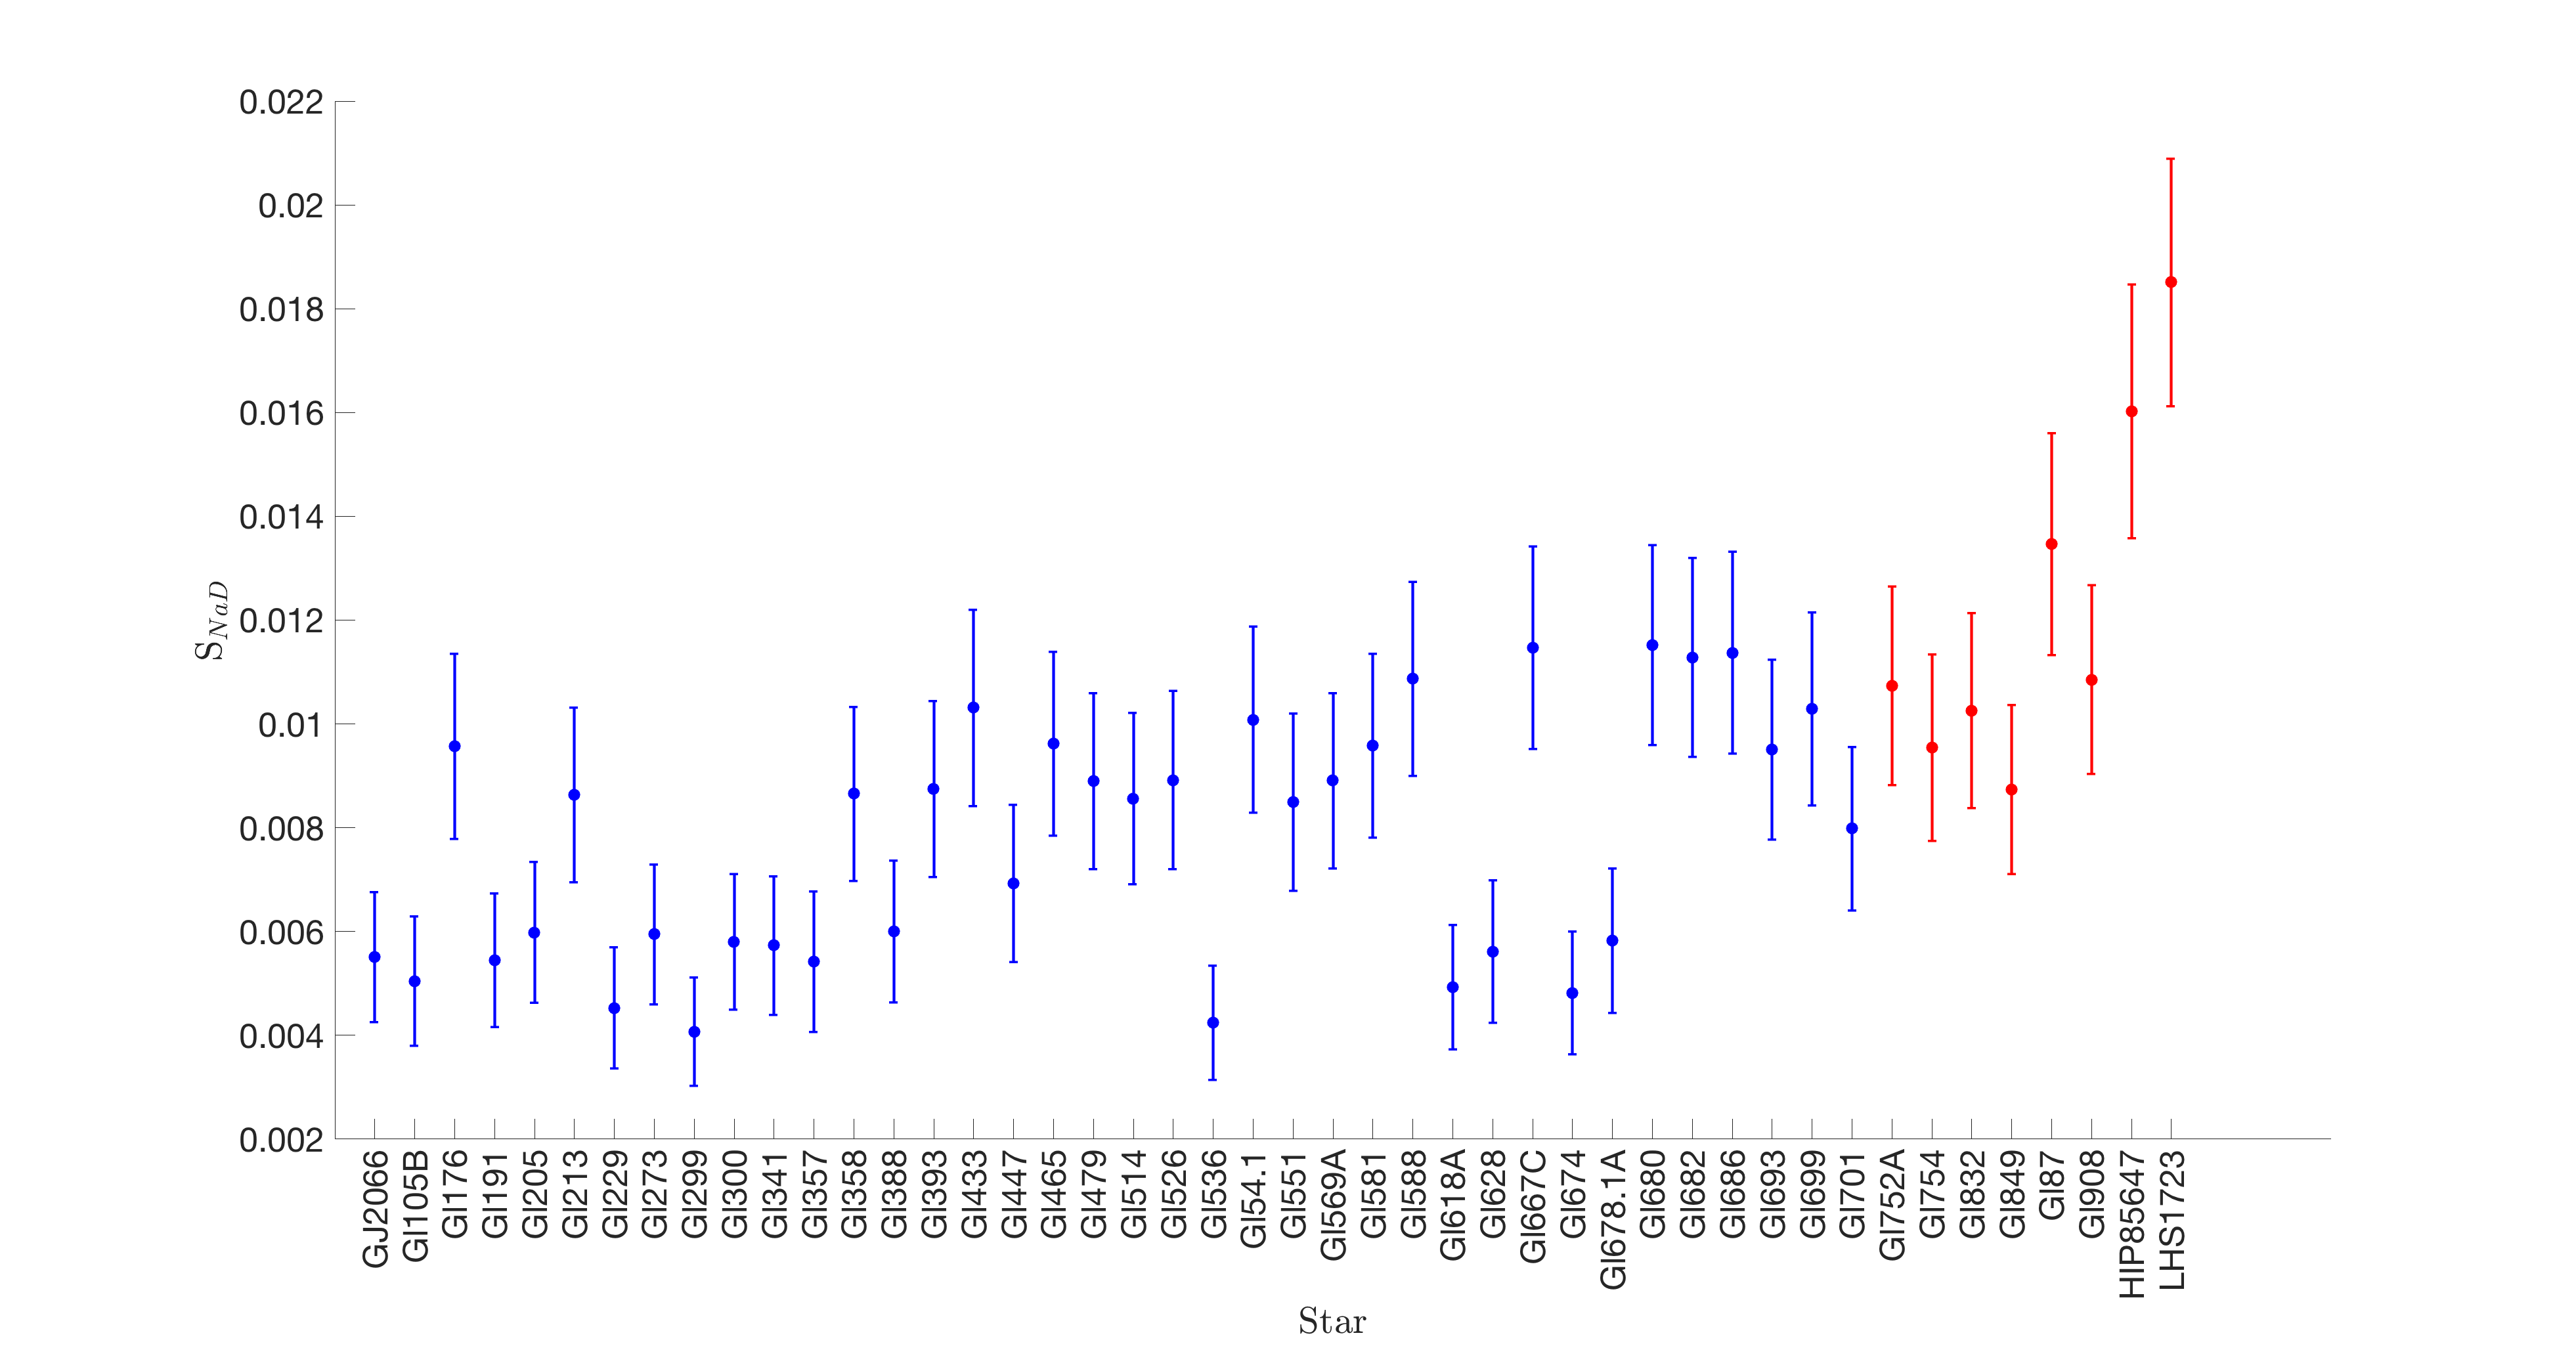
\includegraphics[width=\textwidth]{NaD.png}
    \caption{Median index values for Na\,\textsc{i} D for each of the N stars in the data set, arranged by ascending Ca H\&K S-index value.}
    \label{figNaD}
\end{sidewaysfigure}

\section{Results}
\label{secResults}
Forty-nine stars from Table\,\ref{tabHARPS} had at least 20 observations in the HARPS archive and passed the criteria described in Section\,\ref{secISVmethod}. These stars were processed, ISV spectra produced, and each line above the threshold was identified and measured. Three of these stars, GL1, GL367, and GL382 contained no ISV lines of significance and have been excluded from the analysis. The remaining subsample of 46 M-dwarfs is presented in Table\,\ref{tabHARPSactive}. Included in the table are the median S-indices and uncertainties discussed in Section\,\ref{secOtherInd}. The ISV spectrum for each star in the subsample is presented in Figures\,\ref{figISV1}-\ref{figISV13}. The horizontal red dashed line in each plot is the ISV threshold used for that star, for the selection and analysis as per Section\,\ref{secISVlines}.\\

\begin{figure}[!h]
    \centering
	\captionsetup{width=.8\textwidth}
    \subfloat[]{\label{figISVuncertaintyhistfull}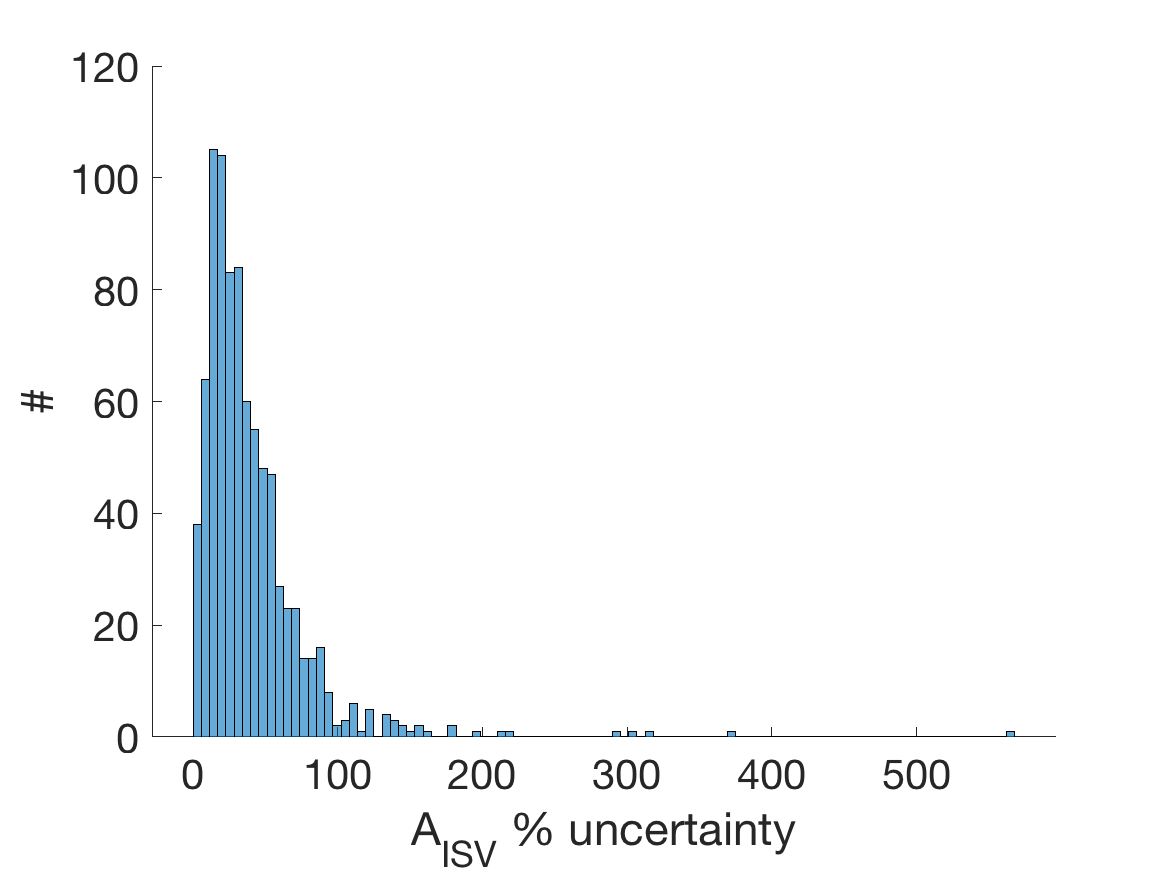
\includegraphics[width=0.8\textwidth]{ISV_uncertainty_hist_full.png}}\\
    \subfloat[]{\label{figISVuncertaintyhistzoom}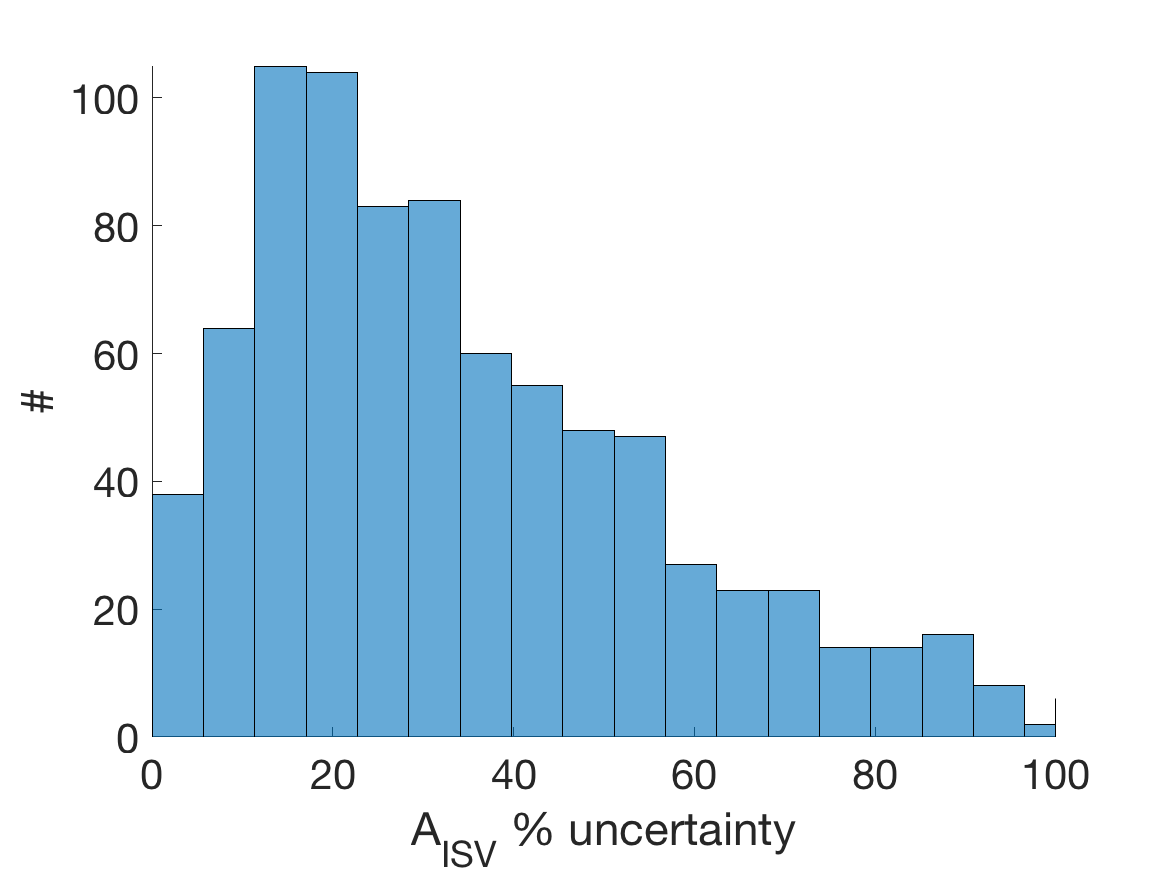
\includegraphics[width=0.8\textwidth]{ISV_uncertainty_hist_zoom.png}}
    \caption{Histogram plot of the percent uncertainty of $A_{ISV}$ for the all the ISV spectral lines in Table\,\ref{tabAllLinesAllStars}.}
    \label{figISVpercentageuncertainty}
\end{figure}

Ninety-seven spectral lines were found to be varying and are presented in Table\,\ref{tabElementFull}. The $A_{ISV}$ values for these lines range from 0.004\hbox{\AA} to 1.214\hbox{\AA}, with a mean value of 0.045\hbox{\AA}. Uncertainties range from \textless1\% to 567\% of their $A_{ISV}$ values with a mean of 40\%. As Figure\,\ref{figISVuncertaintyhistfull} highlights, lines with a percentage uncertainty \textgreater100 are uncommon, and from Figure\,\ref{figISVuncertaintyhistzoom} it is clear that the majority fall with 10-40\%. A 40\% uncertainty on a measurement is significant, and the weak example ISV line shown in Figure\,\ref{figLine2} has a 33\% percent uncertainty. Considering the limited flux at these wavelengths and the weakness of the spectral lines being investigated, this is not surprising. In this data set, weak lines with strong baseline noise are found to be more common than stronger ISV lines like what is presented in Figure\,\ref{figLine1}.\\

\begin{figure}
    \centering
    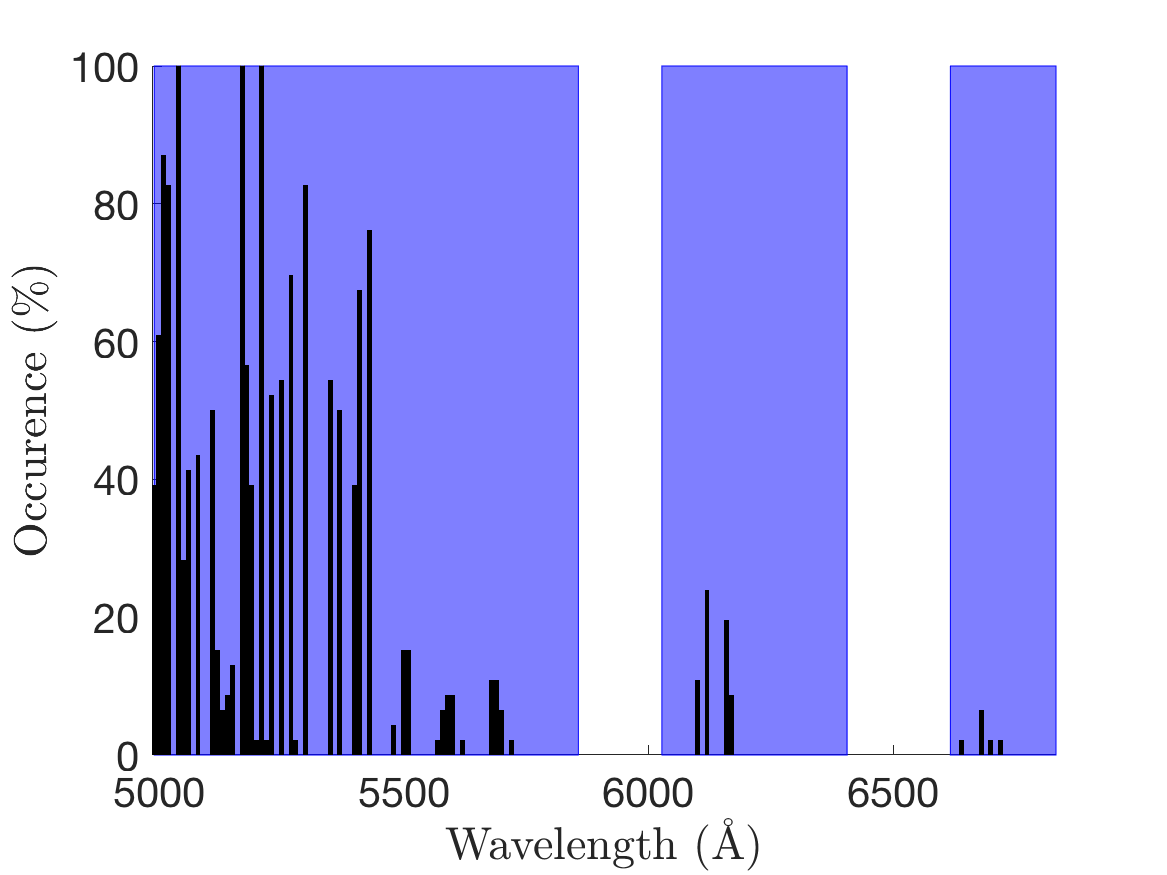
\includegraphics[width=0.8\textwidth]{ISVlineHist.png}
    \caption{The frequency with which a line was found to be varying via the ISV metric in the M-dwarf subsample. The blue background indicates the wavelength regions analysed.}
    \label{figlineHist}
\end{figure}

Figure\,\ref{figlineHist} presents the wavelength distribution of the lines and how frequently ISV variability was detected in the M-dwarf subsample, where ``occurrence'' refers to what percentage of the sample of stars a particular line was found to be varying in. The majority of the varying spectral lines occurred at the blue end of the wavelength range, and bluer lines were also the most frequently varying spectral lines. Of the ninety-seven lines, many were infrequently identified, with more than half detected by ISV analysis in only 1-2 of the 46 stars in the sample. The analysis was restricted to ISV spectral lines that were present in ten or more stars, giving a subsample of thirty seven lines for further study. These lines are presented in Table\,\ref{tabISVlines}.\\

\begin{figure}
    \centering
    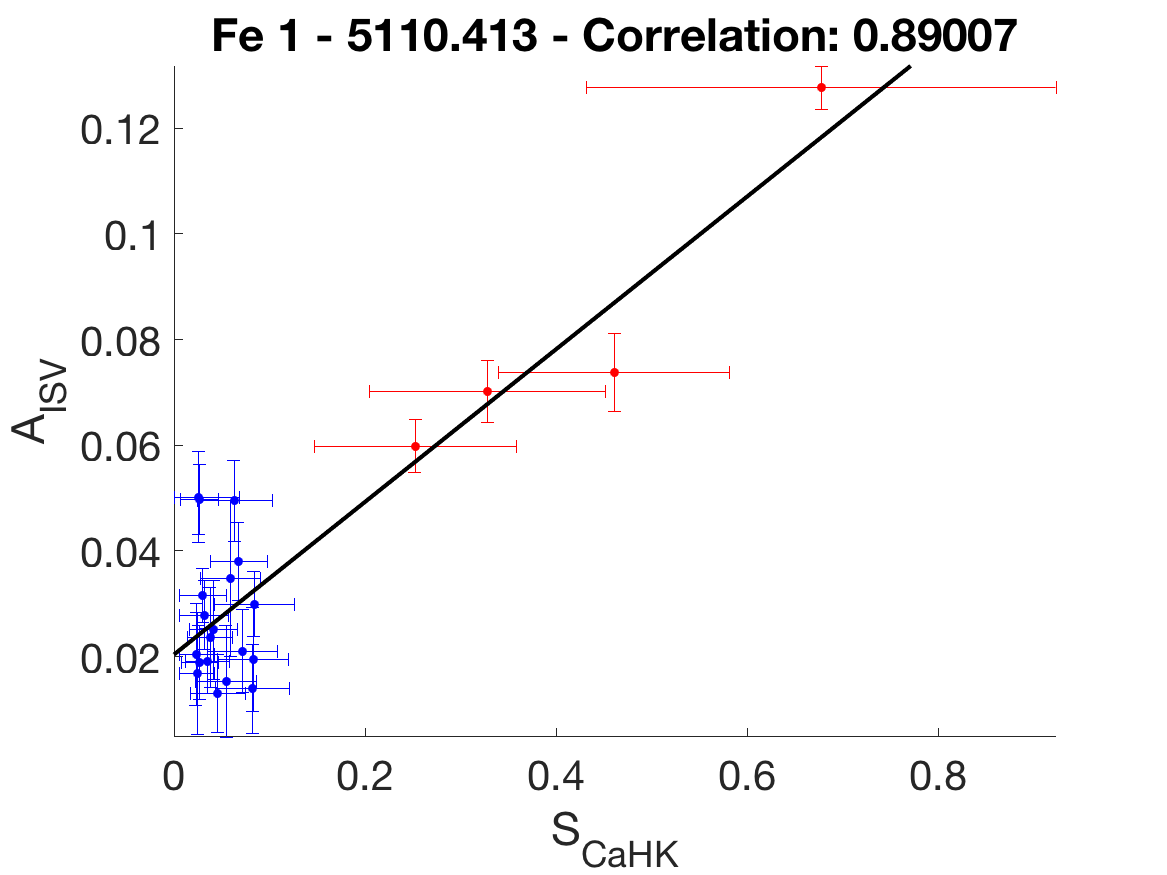
\includegraphics[width=0.8\textwidth]{CorrPlots/CaHK_25.png}
    \caption{A plot of $A_{ISV}$ for the Fe\textsc{I} line at 5110.413\hbox{\AA} and the median S$_{CaHK}$ for each star in the subsample. Blue and red points are the quiescent and active groupings defined in Section\,\ref{secOtherInd} and the black line is the line of best fit between the data. Errorbars are the uncertainties of each quantity, obtained via Equations\,\ref{eqd_A_ISV} and \ref{eqSerr}.}
    \label{figCorrPlotExample}
\end{figure}

Correlations between the $A_{ISV}$ for the thirty-seven ISV selected stellar lines and the Ca\,\textsc{ii} H \& K, H\,\textsc{$\alpha$}, and Na\,\textsc{i} D S-indices were calculated for each star and are included in Table\,\ref{tabISVlines}. High correlation (P\,\textgreater\,0.75) between an ISV spectral line's $A_{ISV}$ and one of the S-indices would suggest that the variability in the line identified by ISV analysis and the line measured for the S-index are produced by the same mechanism. To determine whether the ``active'' and ''quiescent'' S$_{CaHK}$ groupings discussed in Section\,\ref{secOtherInd} are also apparent in the $A_{ISV}$ measurements, plots of the indices were produced. Figure\,\ref{figCorrPlotExample} is an example of one of these plots, comparing the $A_{ISV}$ for a Fe\textsc{I} line, against the median S$_{CaHK}$ for each star in the subsample. The blue points are the quiescent S$_{CaHK}$ stars and the red points are the active S$_{CaHK}$ stars (see Section\,\ref{secOtherInd} for details) and the black line is the linear best fit to the data. The full set of correlation plots is found in Section\,\ref{secCorrPlots}. In general, the active and quiescent S$_{CaHK}$ stars are also active and quiescent in $A_{ISV}$.\\

Looking at Table\,\ref{tabISVlines}, several conclusions can be drawn. The first item of note is that $A_{ISV}$ correlates best with S$_{H\alpha}$. The mean correlation coefficients between S$_{CaHK}$, S$_{H\alpha}$, and S$_{NaD}$ and $A_{ISV}$ are 0.635, 0.723, and 0.391 respectively. There were several lines with poor correlation (P\,\textless\,0.50) in all three indices. These lines were in the regions discussed in Section\,\ref{secISVfeatures} that produced a non-flat ISV noise baseline. Comparing the plots in Section\,\ref{secCorrPlots}, the $A_{ISV}$ values for lines with low correlation have a large scatter, whereas the lines with high correlation have a smaller scatter, centred around low values of $A_{ISV}$.\\

The common active lines of Table\,\ref{tabISVlines} are dominated by transitions of neutral iron, titanium, and chromium. The central wavelengths of these ISV spectral lines agree reasonably well with the known spectral lines. For the transitions to take place the thermal energy at the relevant layer of the star must be sufficient to provide the energy required. For the ISV lines in question this corresponds to a temperature between 3,800\,K, reasonable for the surface of an M dwarf, and \textgreater1x10$^{6}$K, reasonable for the chromosphere. Figure\,\ref{figISVtrans} shows the transition energies ($\Delta E = \frac{hc}{\lambda}$) for each spectral line in Table\,\ref{tabISVlines}, as a function of wavelength. The commonly observed lines are shown as red dots, and the transitions found in \textless10 stars are in black. The horizontal dashed lines represent the thermal energy at the lower bound of the photosphere (5,500K), the upper photosphere/lower chromosphere boundary (3,800K), the lower/upper chromosphere boundary (2,800K), and the transition region (5,000K), for M-dwarfs (see \citealt{2017Linsky} for details). The expected temperature of the upper chromosphere/corona boundary is 2.7x10$^{6}$K $=232.7$ eV, too large to plot on Figure\,\ref{figISVtrans}, and in its place is a 10,000K boundary. While the chromosphere of the Linksy model extends well past this temperature, 10,000K was useful to see how far into the chromosphere the transitions took place. The energy requirements for these transitions range from 1.8 to 2.5 eV, meaning that they must be produced in regions \textgreater5,500\,K. The ionisation potential for each line was determined and plotted in Figure\,\ref{figISVion}, with the same mean thermal energy regions as Figure\,\ref{figISVtrans}. The temperatures required to ionise these elements are much greater than any of the identified regions, but less than the 232.eV produced at the upper chromosphere/corona boundary. Taking these two limits into consideration, the only region that can produce the expected transitions is the upper chromosphere. Supporting this conclusion, the S-index most sensitive to the upper chromosphere is H $\alpha$, which is also the S-index with the greatest mean correlation in Table\,\ref{tabISVlines}.\\

\begin{figure}[!h]
    \centering
	\captionsetup{width=.8\textwidth}
    \subfloat[]{\label{figISVtrans}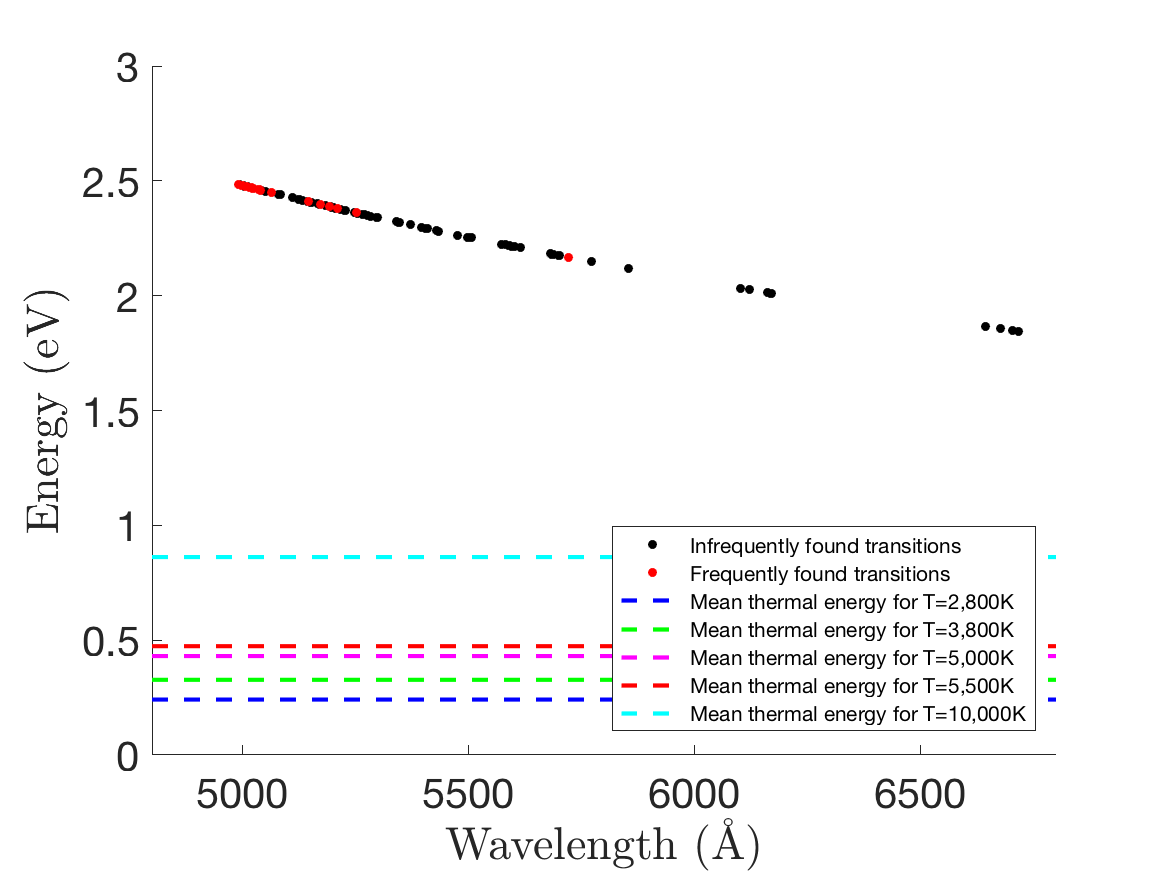
\includegraphics[width=0.8\textwidth]{LineTransitions.png}}\\
    \subfloat[]{\label{figISVion}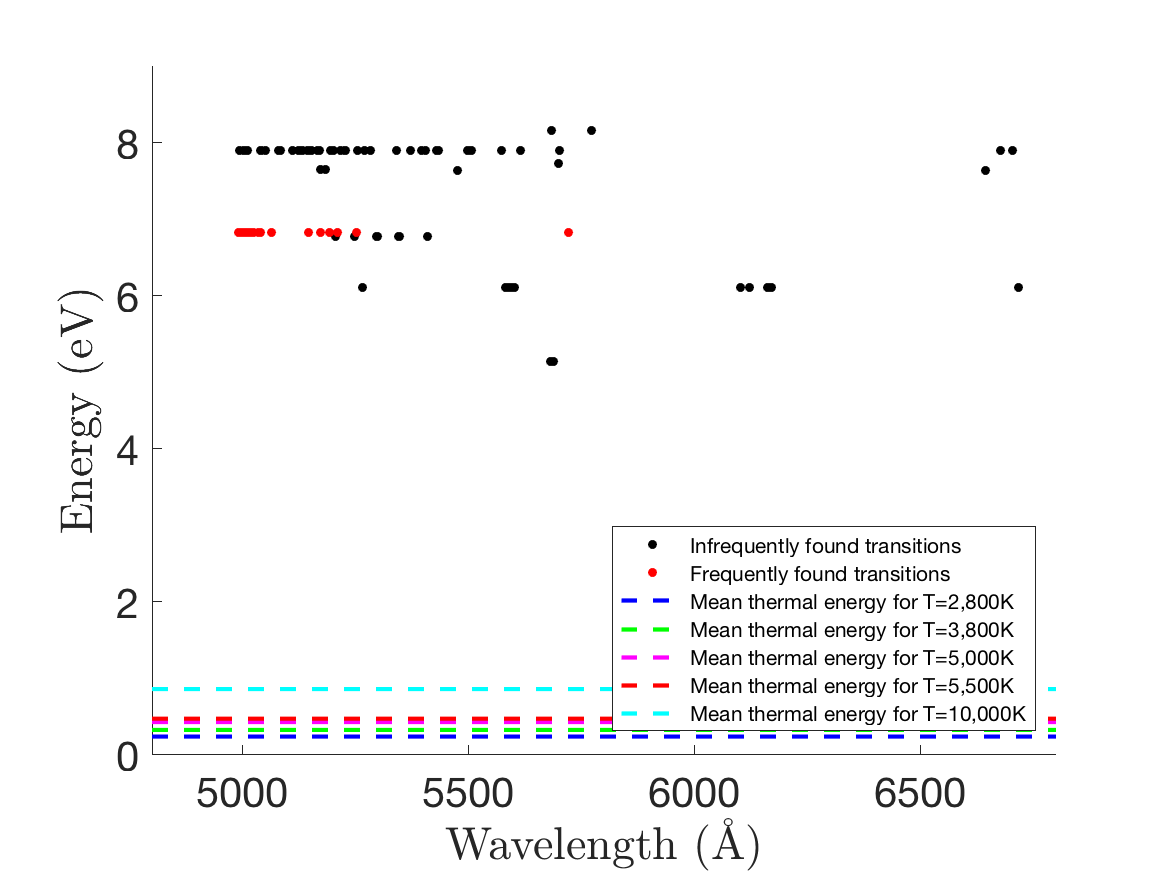
\includegraphics[width=0.8 \textwidth]{LineIonisations.png}}
    \caption{Plots determining the transition energy (left) and ionisation potential (right) of the active lines from Table\,\ref{tabISVlines}. The red, green, blue, magenta, and cyan dashed lines represent the mean thermal energy at T\,=\,2,800, 3,800, 5,000, 5,500, and 10,000K.}
    \label{figLineTransIon}
\end{figure}

\subsection{The M-dwarf subsample}
\begin{landscape}
    \begin{longtable}{|c|c|c|c|c|c|c|c|c|c|}
    \captionsetup{width=1.4\textwidth}
    \hline
    Designation & Spectral & Observations & \multicolumn{2}{c|}{MJD} & Nights & Range & S$_{CaHK}$ & S$_{H\alpha}$ & S$_{NaD}$\\
    \cline{4-5}
     & Class & (\#) & Start & End & & (yrs) &  &  & \\
    \hline
    \endfirsthead
    
    \hline
    Designation & Spectral & Observations & \multicolumn{2}{c|}{MJD} & Nights & Range & S$_{CaHK}$ & S$_{H\alpha}$ & S$_{NaD}$\\
    \cline{4-5}
     & Class & (\#) & Start & End & & (yrs) &  &  & \\
    \hline
    \endhead
    
    \hline
    \caption{Stars from the HARPS M-dwarf sample (Table\,\ref{tabHARPS}) with at least 20 observations and at least 3 lines found to be variable in the ISV spectra. MJD is the Julian date minus 2,450,000 days of the first and last observation. Nights is the total number of nights each star was observed and Range is the time span in years for all observations. The S-index values represent the median value taken across all observations and the uncertainty is the standard deviation.}
    \endfoot
    
GJ2066 & M2 & 84 & 2987.79 & 7115.54 & 81 & 11.3 & 0.044 $\pm$ 0.027 & 0.073 $\pm$ 0.004 & 0.009 $\pm$ 0.002\\    
GL105B & M3.5 & 22 & 2986.61 & 5414.94 & 22 & 6.6 & 0.035 $\pm$ 0.02 & 0.076 $\pm$ 0.004 & 0.005 $\pm$ 0.001\\    
GL176 & M2.5 & 71 & 2986.71 & 5132.81 & 71 & 5.9 & 0.083 $\pm$ 0.037 & 0.075 $\pm$ 0.004 & 0.01 $\pm$ 0.002\\     
GL191 & M1 & 96 & 2985.74 & 6667.8 & 48 & 10.1 & 0.018 $\pm$ 0.017 & 0.076 $\pm$ 0.004 & 0.006 $\pm$ 0.001\\      
GL205 & M1.5 & 76 & 2986.73 & 4386.81 & 66 & 3.8 & 0.109 $\pm$ 0.043 & 0.072 $\pm$ 0.004 & 0.011 $\pm$ 0.002\\    
GL213 & M4 & 46 & 2986.74 & 7117.48 & 46 & 11.3 & 0.027 $\pm$ 0.02 & 0.076 $\pm$ 0.004 & 0.005 $\pm$ 0.001\\      
GL229 & M1 & 121 & 2986.75 & 7144.46 & 115 & 11.4 & 0.079 $\pm$ 0.038 & 0.071 $\pm$ 0.004 & 0.011 $\pm$ 0.002\\   
GL273 & M3.5 & 225 & 2986.77 & 7144.47 & 198 & 11.4 & 0.038 $\pm$ 0.023 & 0.077 $\pm$ 0.004 & 0.006 $\pm$ 0.001\\ 
GL299 & M4.5 & 20 & 2986.79 & 5626.59 & 20 & 7.2 & 0.048 $\pm$ 0.026 & 0.077 $\pm$ 0.004 & 0.004 $\pm$ 0.001\\    
GL300 & M3.5 & 39 & 2986.8 & 5309.48 & 37 & 6.4 & 0.068 $\pm$ 0.03 & 0.079 $\pm$ 0.004 & 0.006 $\pm$ 0.001\\      
GL341 & M0 & 57 & 2985.79 & 6316.85 & 57 & 9.1 & 0.073 $\pm$ 0.039 & 0.072 $\pm$ 0.004 & 0.011 $\pm$ 0.002\\      
GL357 & M2.5 & 49 & 3815.72 & 6336.79 & 49 & 6.9 & 0.025 $\pm$ 0.044 & 0.075 $\pm$ 0.004 & 0.006 $\pm$ 0.001\\    
GL358 & M3 & 34 & 3669.84 & 6325.84 & 34 & 7.3 & 0.169 $\pm$ 0.058 & 0.102 $\pm$ 0.005 & 0.01 $\pm$ 0.002\\       
GL388 & M4 & 46 & 2986.86 & 6659.85 & 39 & 10.1 & 0.461 $\pm$ 0.121 & 0.163 $\pm$ 0.007 & 0.016 $\pm$ 0.002\\     
GL393 & M2 & 137 & 2986.86 & 7146.61 & 135 & 11.4 & 0.049 $\pm$ 0.028 & 0.074 $\pm$ 0.004 & 0.009 $\pm$ 0.002\\   
GL433 & M2 & 86 & 2989.84 & 6001.66 & 83 & 8.2 & 0.042 $\pm$ 0.025 & 0.072 $\pm$ 0.004 & 0.01 $\pm$ 0.002\\       
GL447 & M4 & 131 & 3578.46 & 7139.66 & 127 & 9.8 & 0.064 $\pm$ 0.039 & 0.078 $\pm$ 0.004 & 0.005 $\pm$ 0.001\\    
GL465 & M2 & 20 & 3159.62 & 6058.69 & 20 & 7.9 & 0.02 $\pm$ 0.016 & 0.075 $\pm$ 0.004 & 0.005 $\pm$ 0.001\\       
GL479 & M3 & 58 & 3158.54 & 4571.69 & 58 & 3.9 & 0.111 $\pm$ 0.043 & 0.085 $\pm$ 0.004 & 0.01 $\pm$ 0.002\\       
GL514 & M1 & 139 & 3152.62 & 7115.72 & 131 & 10.9 & 0.055 $\pm$ 0.032 & 0.071 $\pm$ 0.004 & 0.011 $\pm$ 0.002\\   
GL526 & M2 & 32 & 3158.59 & 6837.55 & 32 & 10.1 & 0.039 $\pm$ 0.022 & 0.072 $\pm$ 0.004 & 0.01 $\pm$ 0.002\\      
GL536 & M0 & 139 & 3158.61 & 7148.74 & 135 & 10.9 & 0.06 $\pm$ 0.033 & 0.072 $\pm$ 0.004 & 0.011 $\pm$ 0.002\\     
GL54.1 & M4 & 89 & 2996.56 & 7050.53 & 87 & 11.1 & 0.328 $\pm$ 0.123 & 0.111 $\pm$ 0.004 & 0.011 $\pm$ 0.002\\    
GL551 & M5.5 & 257 & 3152.6 & 6667.87 & 88 & 9.6 & 0.678 $\pm$ 0.246 & 0.134 $\pm$ 0.004 & 0.019 $\pm$ 0.002\\    
GL569A & M3 & 25 & 3158.62 & 6335.89 & 25 & 8.7 & 0.264 $\pm$ 0.102 & 0.107 $\pm$ 0.005 & 0.013 $\pm$ 0.002\\     
GL581 & M3 & 242 & 3152.71 & 6061.68 & 235 & 8 & 0.024 $\pm$ 0.018 & 0.077 $\pm$ 0.004 & 0.005 $\pm$ 0.001\\      
GL588 & M2.5 & 257 & 3152.75 & 7163.8 & 56 & 11 & 0.046 $\pm$ 0.029 & 0.075 $\pm$ 0.004 & 0.009 $\pm$ 0.002\\     
GL618A & M3 & 21 & 3158.69 & 5630.84 & 21 & 6.8 & 0.039 $\pm$ 0.029 & 0.074 $\pm$ 0.004 & 0.007 $\pm$ 0.002\\     
GL628 & M3 & 164 & 3158.67 & 7145.83 & 158 & 10.9 & 0.035 $\pm$ 0.023 & 0.077 $\pm$ 0.004 & 0.006 $\pm$ 0.001\\   
GL667C & M1.5 & 185 & 3158.76 & 6094.74 & 184 & 8 & 0.027 $\pm$ 0.019 & 0.075 $\pm$ 0.004 & 0.006 $\pm$ 0.001\\   
GL674 & M3 & 178 & 3158.75 & 7140.9 & 172 & 10.9 & 0.084 $\pm$ 0.042 & 0.084 $\pm$ 0.004 & 0.008 $\pm$ 0.002\\    
GL678.1A & M1 & 123 & 3159.73 & 7143.76 & 121 & 10.9 & 0.072 $\pm$ 0.037 & 0.072 $\pm$ 0.004 & 0.012 $\pm$ 0.002\\
GL680 & M3 & 39 & 3159.71 & 6167.51 & 39 & 8.2 & 0.047 $\pm$ 0.027 & 0.073 $\pm$ 0.004 & 0.009 $\pm$ 0.002\\      
GL682 & M3.5 & 20 & 3205.67 & 6101.57 & 20 & 7.9 & 0.059 $\pm$ 0.032 & 0.078 $\pm$ 0.004 & 0.006 $\pm$ 0.001\\    
GL686 & M1.5 & 20 & 3159.74 & 5458.51 & 20 & 6.3 & 0.035 $\pm$ 0.024 & 0.073 $\pm$ 0.004 & 0.009 $\pm$ 0.002\\    
GL693 & M3.5 & 128 & 3201.65 & 7147.92 & 124 & 10.8 & 0.031 $\pm$ 0.026 & 0.076 $\pm$ 0.004 & 0.006 $\pm$ 0.001\\ 
GL699 & M4 & 233 & 4194.89 & 6428.93 & 114 & 6.1 & 0.03 $\pm$ 0.025 & 0.076 $\pm$ 0.004 & 0.004 $\pm$ 0.001\\     
GL701 & M0 & 117 & 3158.81 & 7147.91 & 116 & 10.9 & 0.049 $\pm$ 0.03 & 0.072 $\pm$ 0.004 & 0.01 $\pm$ 0.002\\     
GL752A & M3 & 107 & 3159.81 & 6936.53 & 105 & 10.3 & 0.051 $\pm$ 0.034 & 0.073 $\pm$ 0.004 & 0.01 $\pm$ 0.002\\   
GL754 & M4.5 & 121 & 3154.83 & 6926.6 & 116 & 10.3 & 0.057 $\pm$ 0.038 & 0.077 $\pm$ 0.004 & 0.005 $\pm$ 0.001\\  
GL832 & M2.5 & 61 & 2985.52 & 6119.85 & 61 & 8.6 & 0.039 $\pm$ 0.026 & 0.073 $\pm$ 0.004 & 0.009 $\pm$ 0.002\\    
GL849 & M3.5 & 48 & 2990.55 & 5814.73 & 48 & 7.7 & 0.049 $\pm$ 0.027 & 0.073 $\pm$ 0.004 & 0.008 $\pm$ 0.002\\    
GL87 & M1 & 96 & 2988.64 & 7051.53 & 95 & 11.1 & 0.024 $\pm$ 0.018 & 0.074 $\pm$ 0.004 & 0.01 $\pm$ 0.002\\
GL908 & M1 & 87 & 2986.58 & 6263.58 & 87 & 9 & 0.026 $\pm$ 0.018 & 0.073 $\pm$ 0.004 & 0.009 $\pm$ 0.002\\
HIP85647 & M0 & 123 & 4167.9 & 7148.82 & 115 & 8.2 & 0.082 $\pm$ 0.039 & 0.069 $\pm$ 0.004 & 0.01 $\pm$ 0.002\\   
LHS1723 & M4 & 123 & 2986.72 & 7117.49 & 116 & 11.3 & 0.253 $\pm$ 0.106 & 0.102 $\pm$ 0.004 & 0.009 $\pm$ 0.002
    \label{tabHARPSactive}
    \end{longtable}
\end{landscape}

\subsection{ISV plots}
\begin{figure}[!h]
    \subfloat[GJ2066]{\label{figISV1}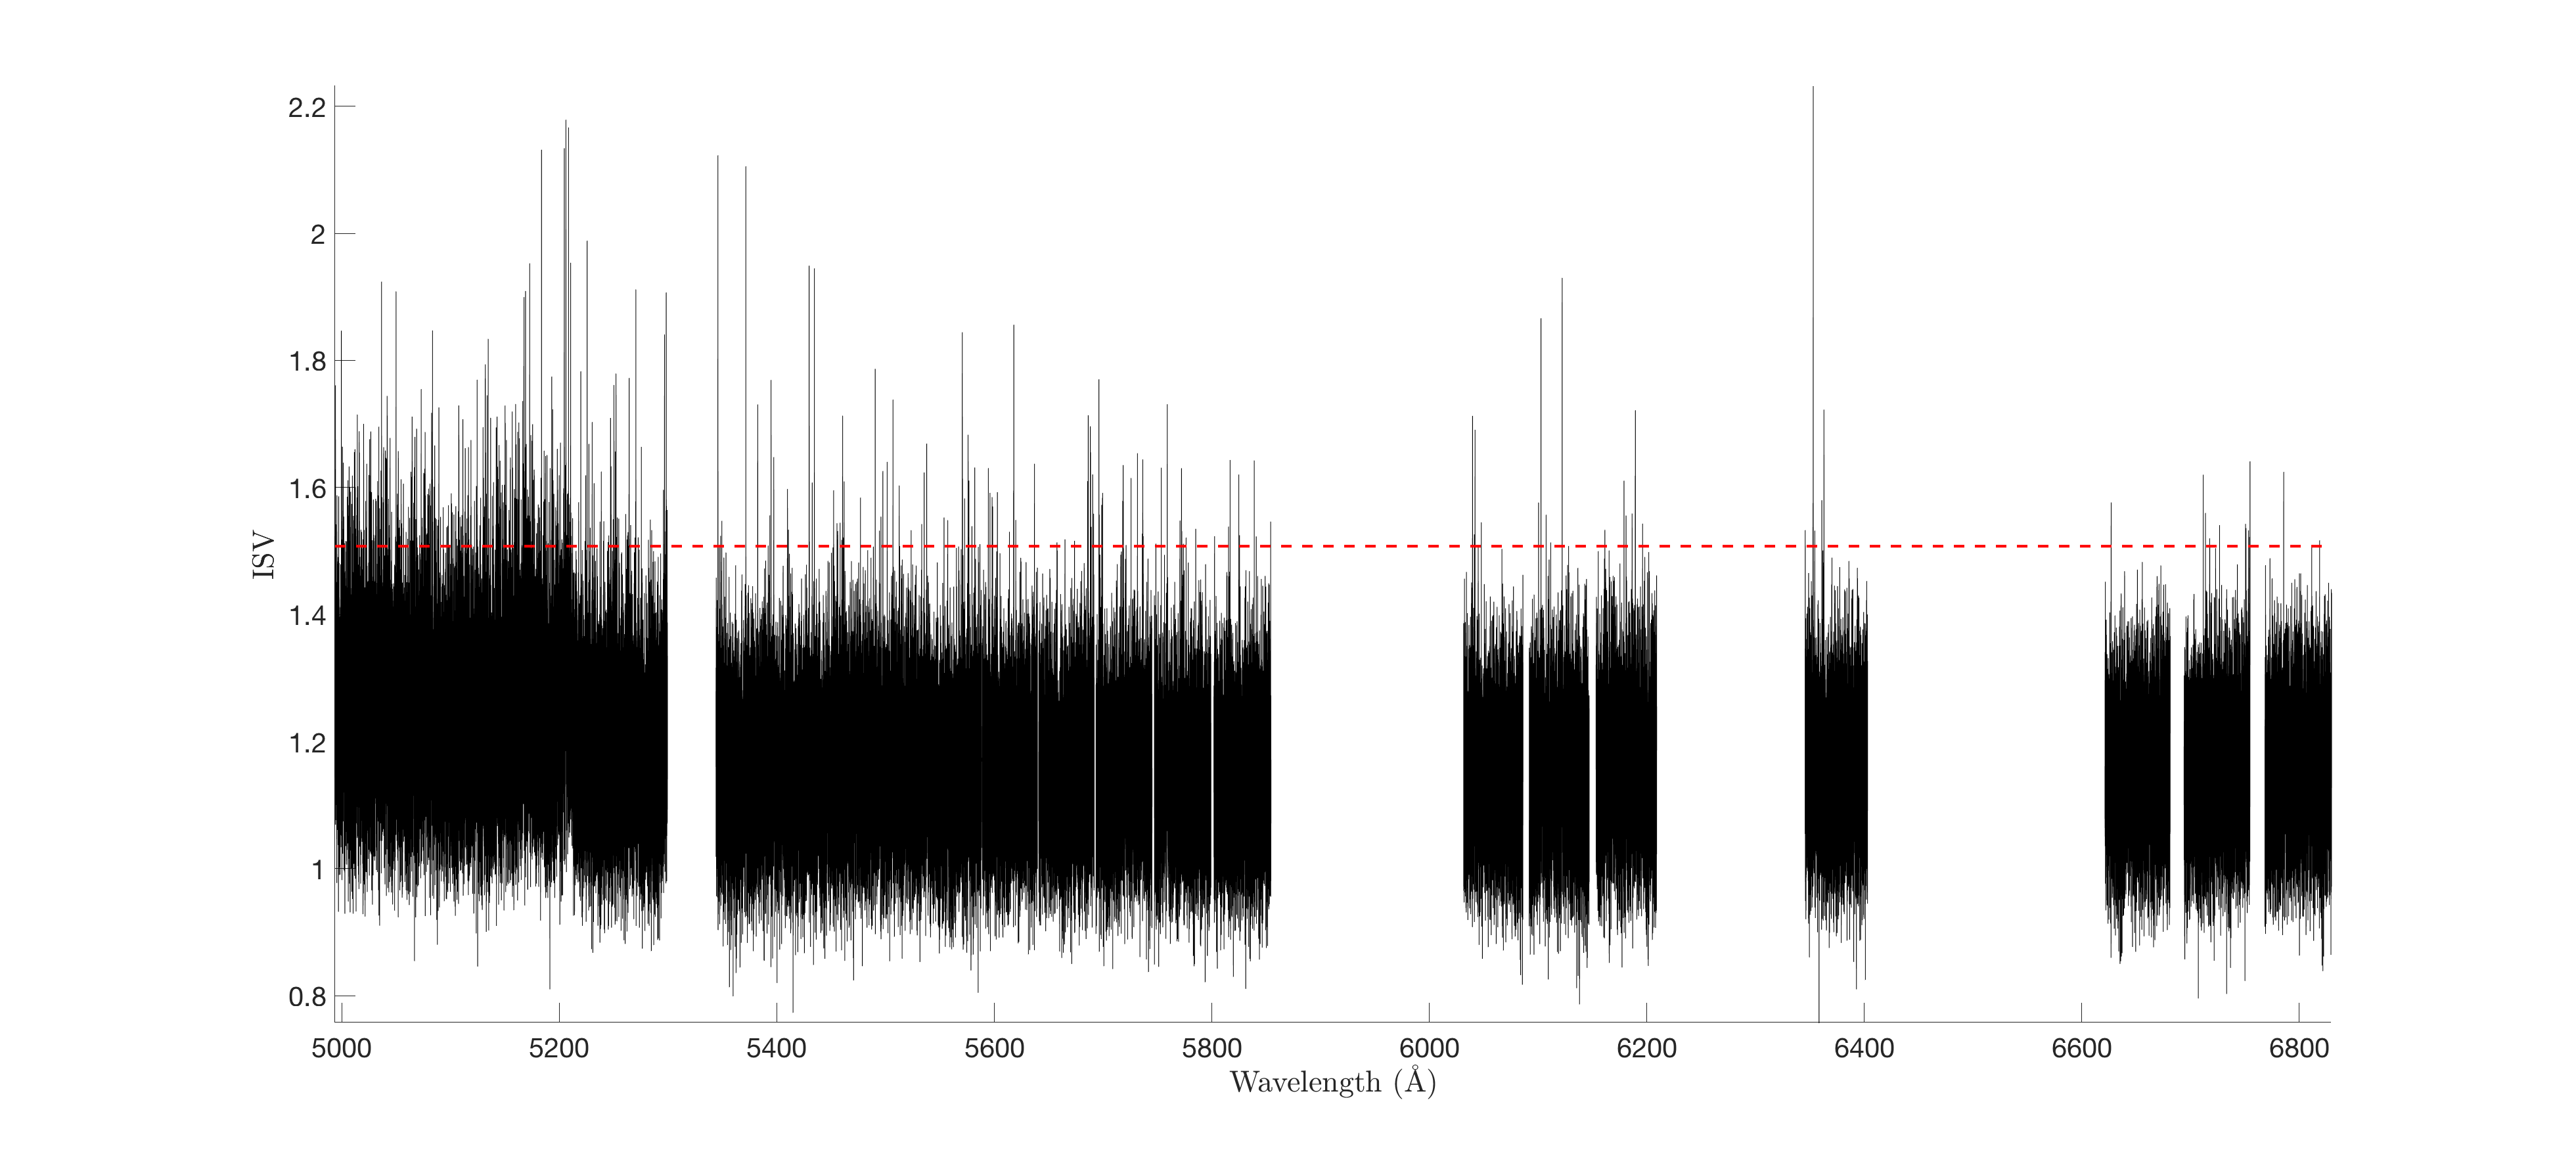
\includegraphics[width=1\textwidth]{ISVplots/thesis_GJ2066.png}}\\
    \subfloat[GL1]{\label{figISV2}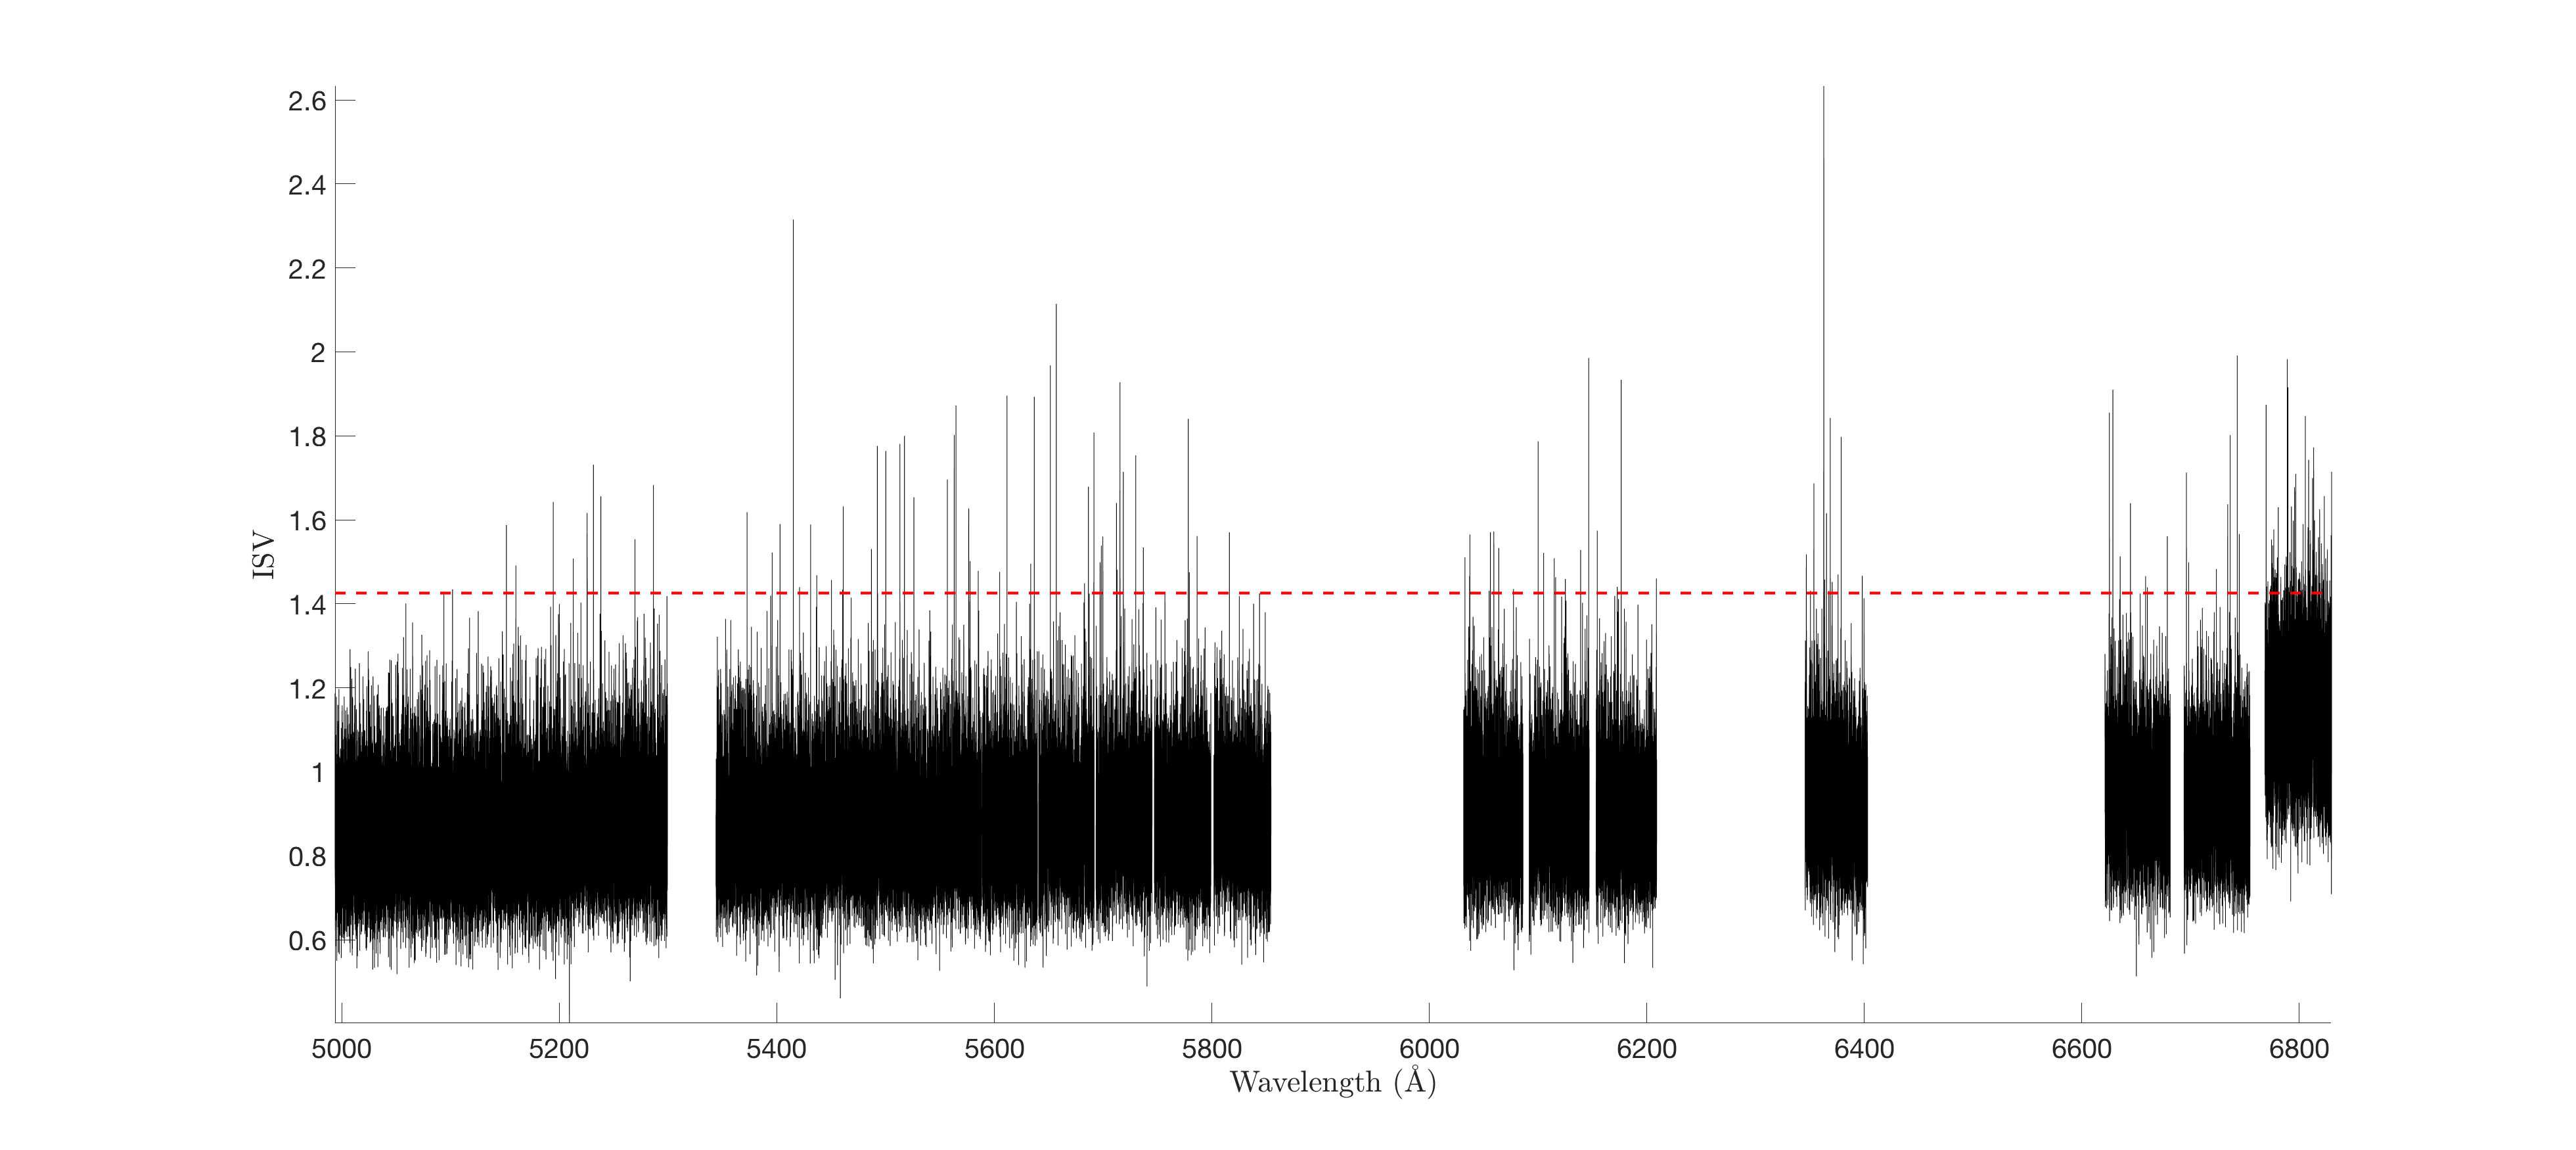
\includegraphics[width=1\textwidth]{ISVplots/thesis_Gl1.png}}\\
    \subfloat[GL105B]{\label{figISV3}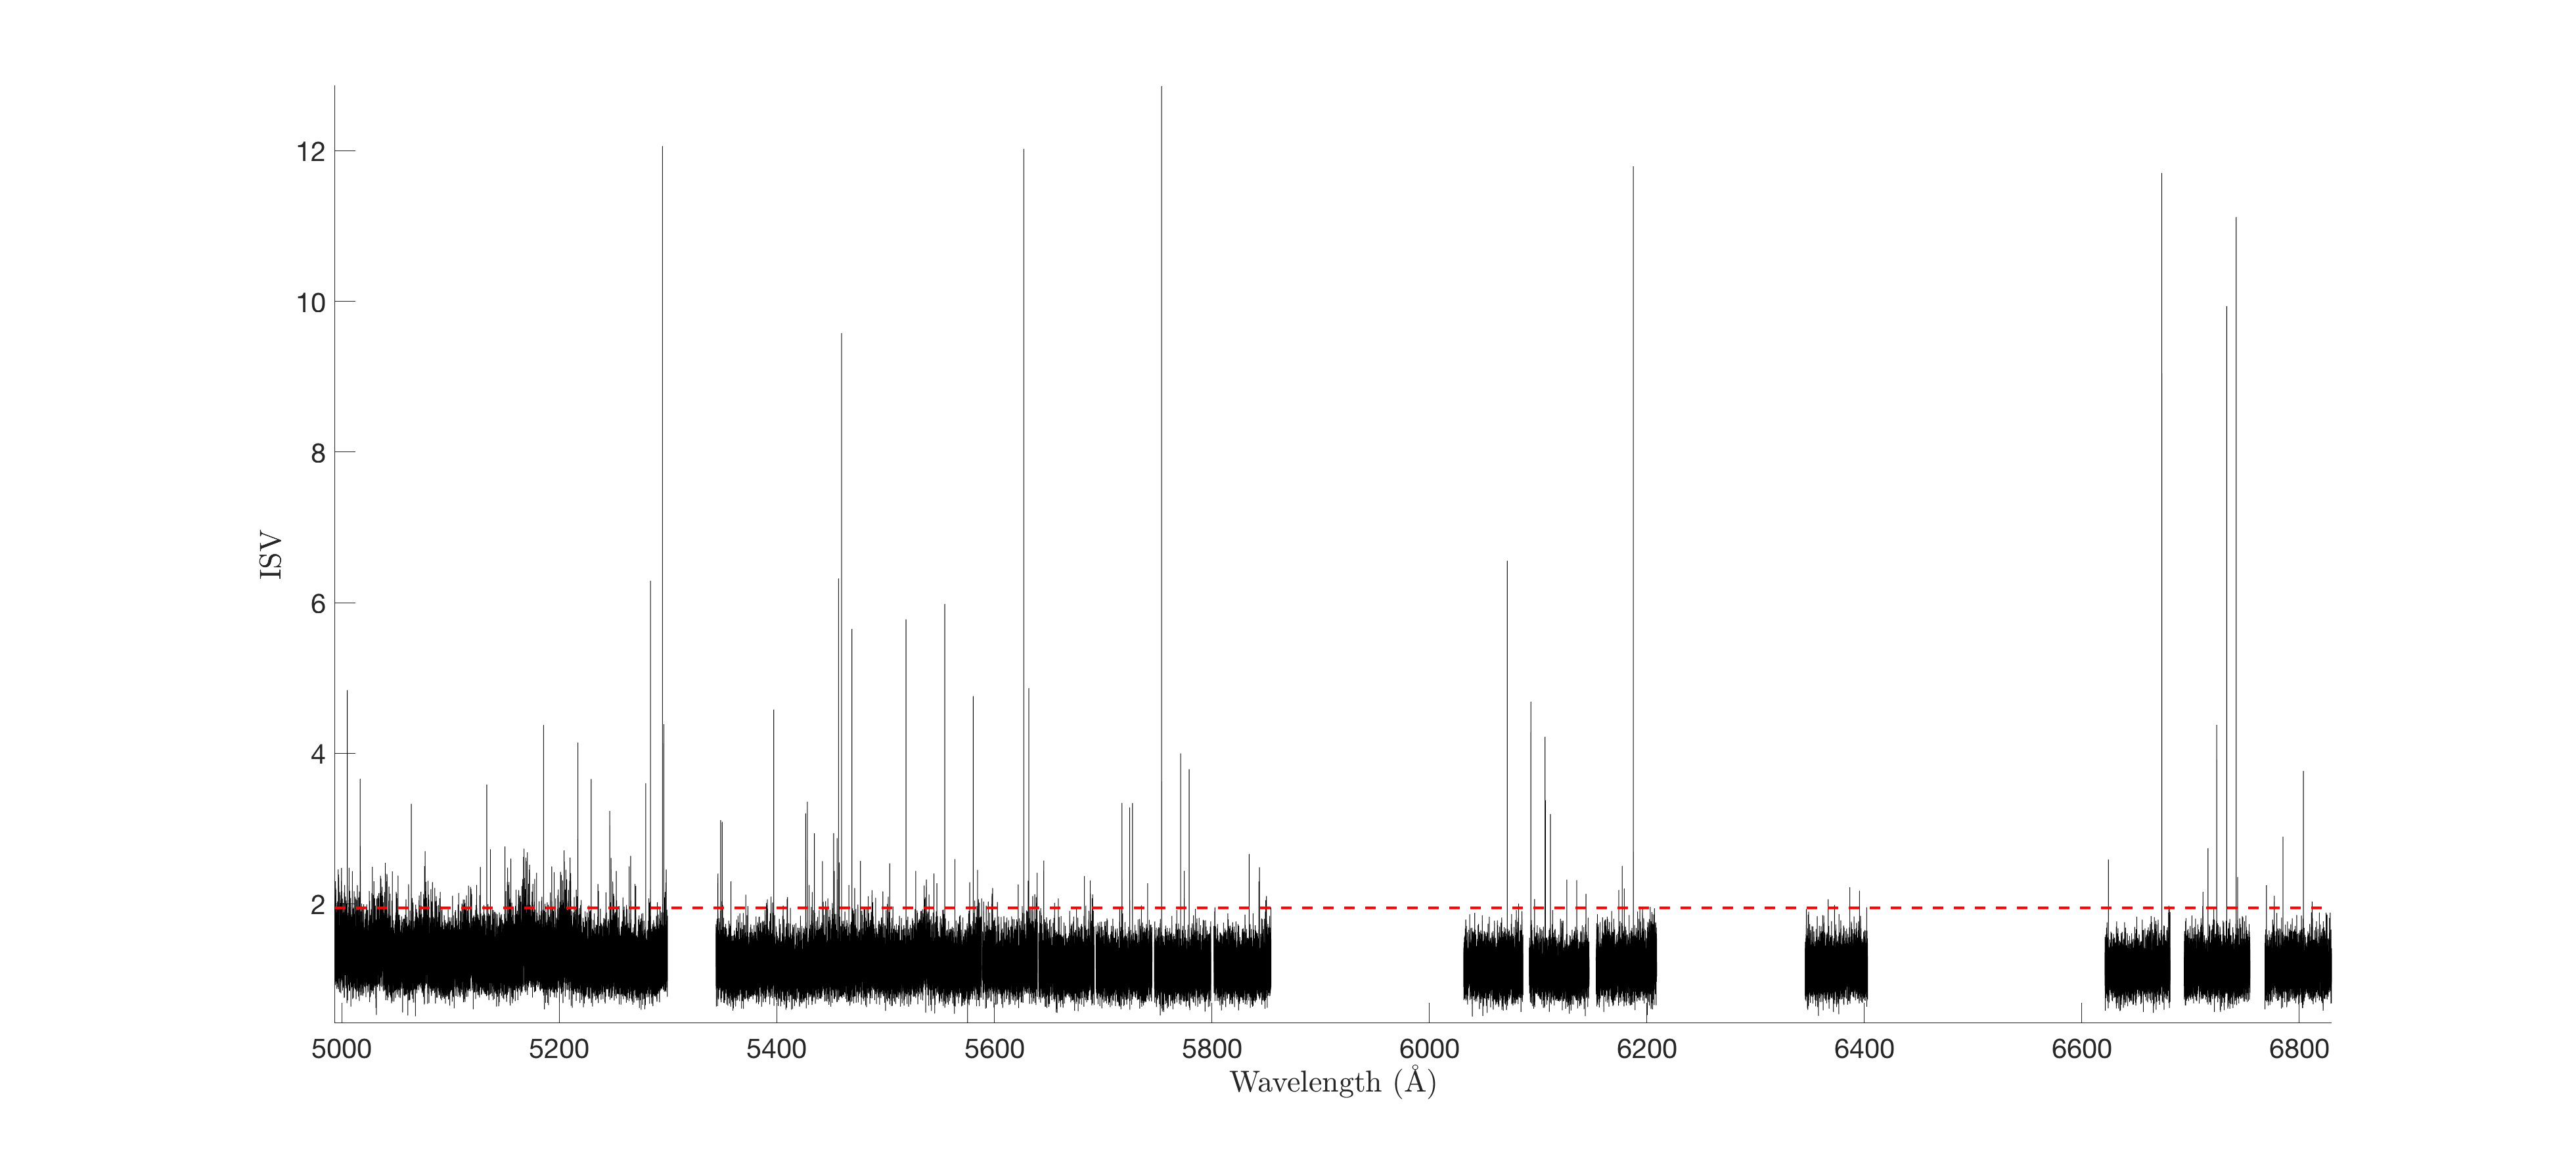
\includegraphics[width=1\textwidth]{ISVplots/thesis_Gl105B.png}}
    \caption{The `spectra' represents the variation per-pixel between all spectra taken for a star in the HARPS M-dwarf sample. The horizontal red dashed line indicates the threshold between significant variation and the baseline noise due to photometric noise varying between spectra.}
\end{figure}

\begin{figure}
    \subfloat[GL176]{\label{figISV4}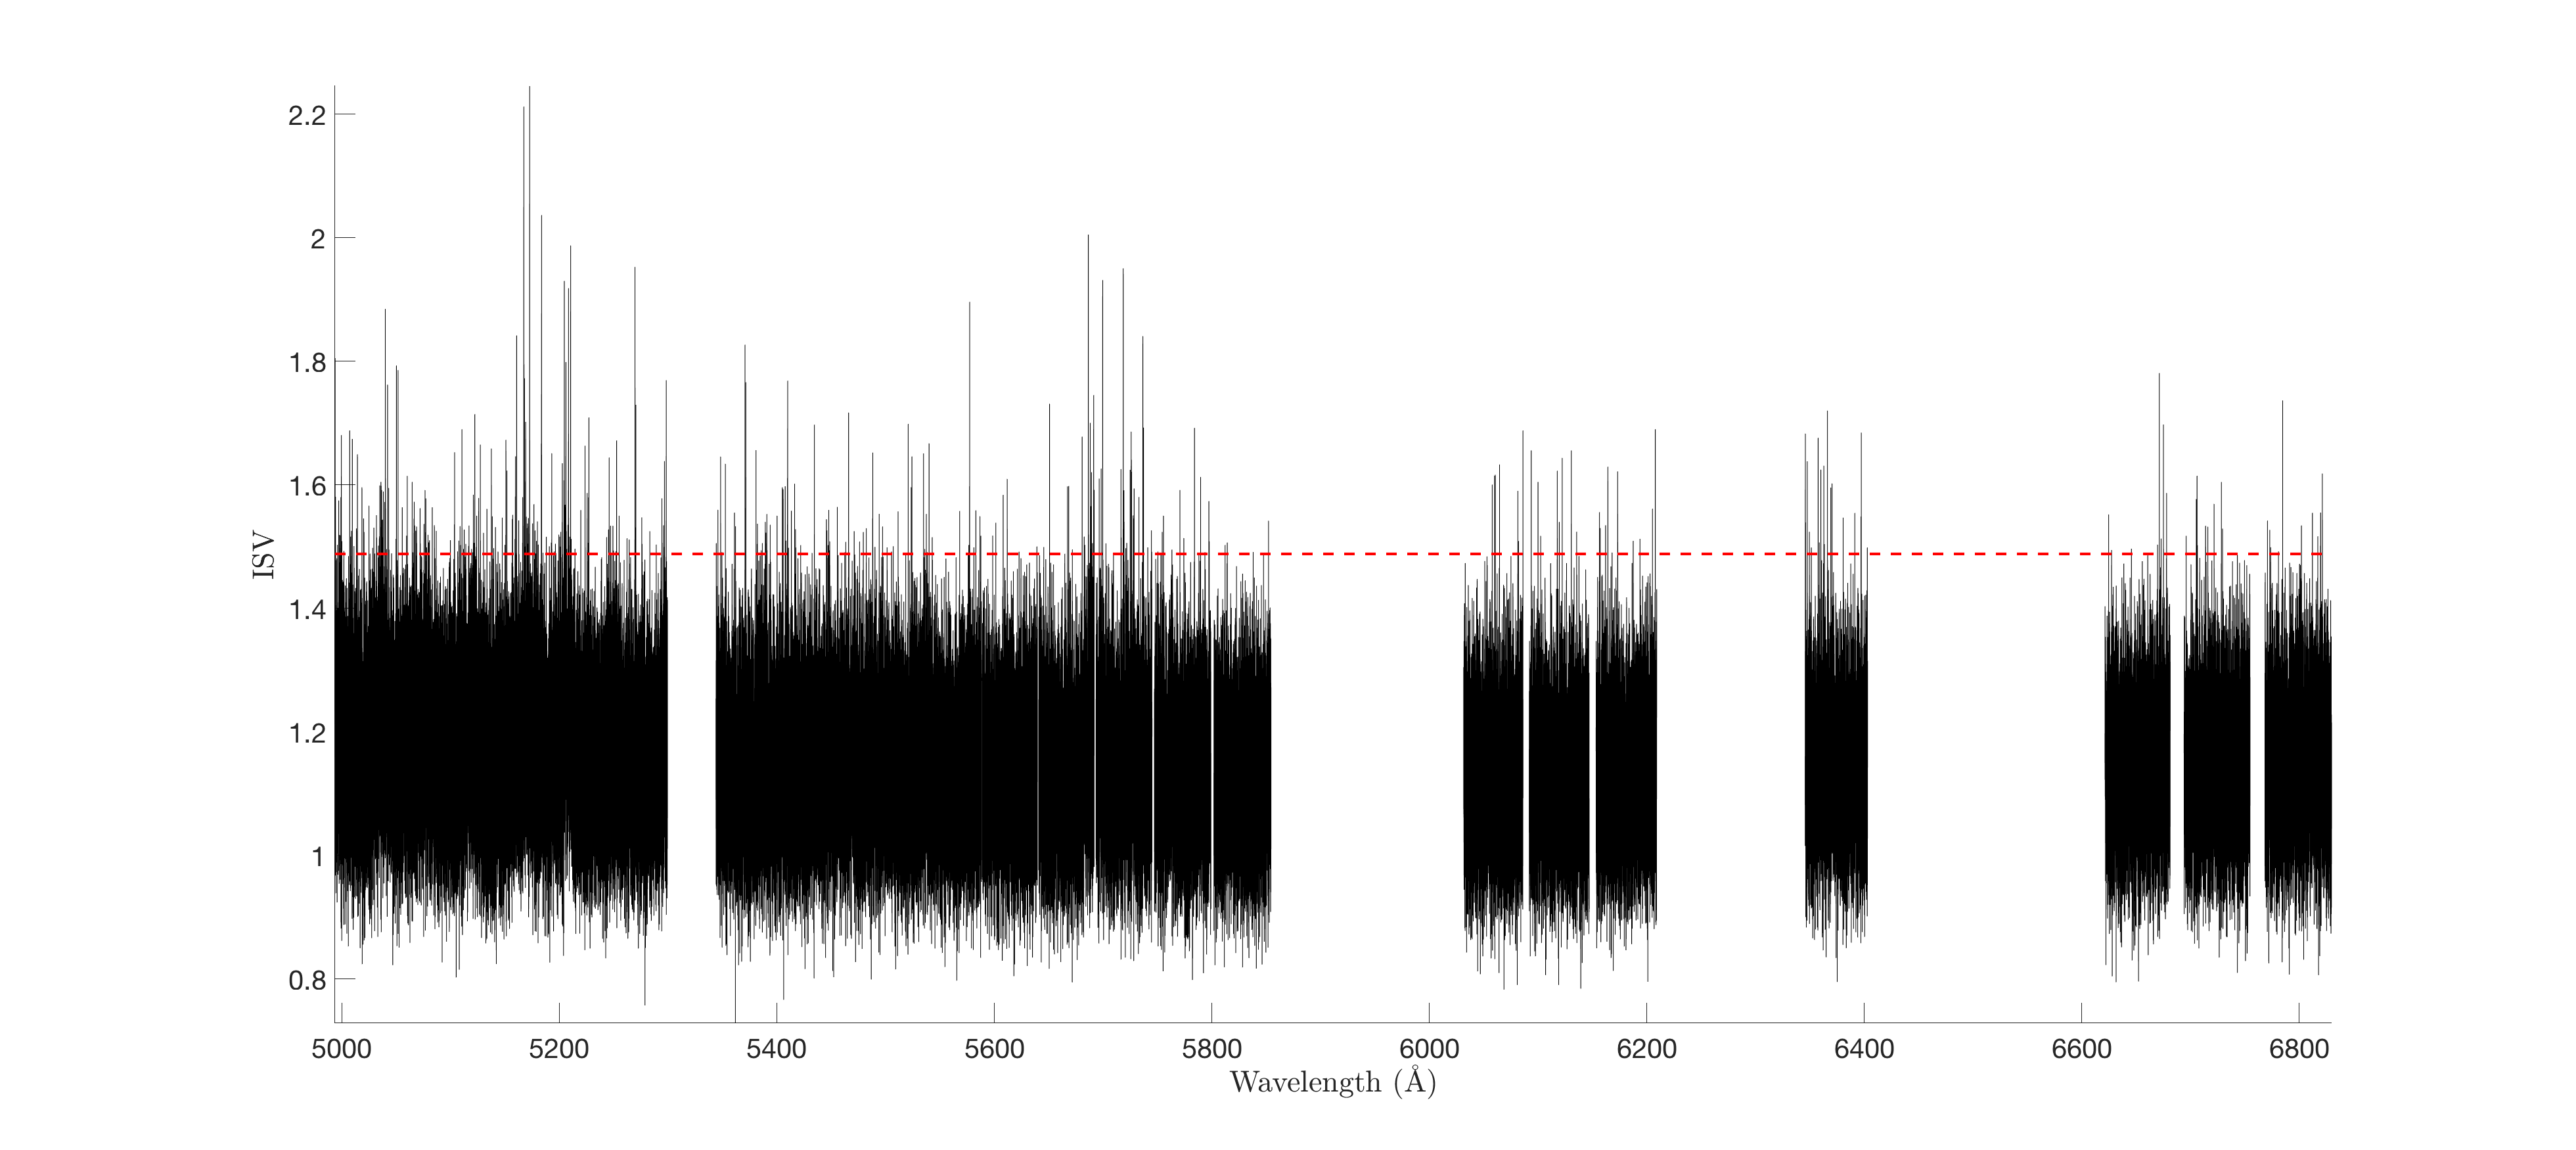
\includegraphics[width=1\textwidth]{ISVplots/thesis_Gl176.png}}\\
    \subfloat[GL191]{\label{figISV5}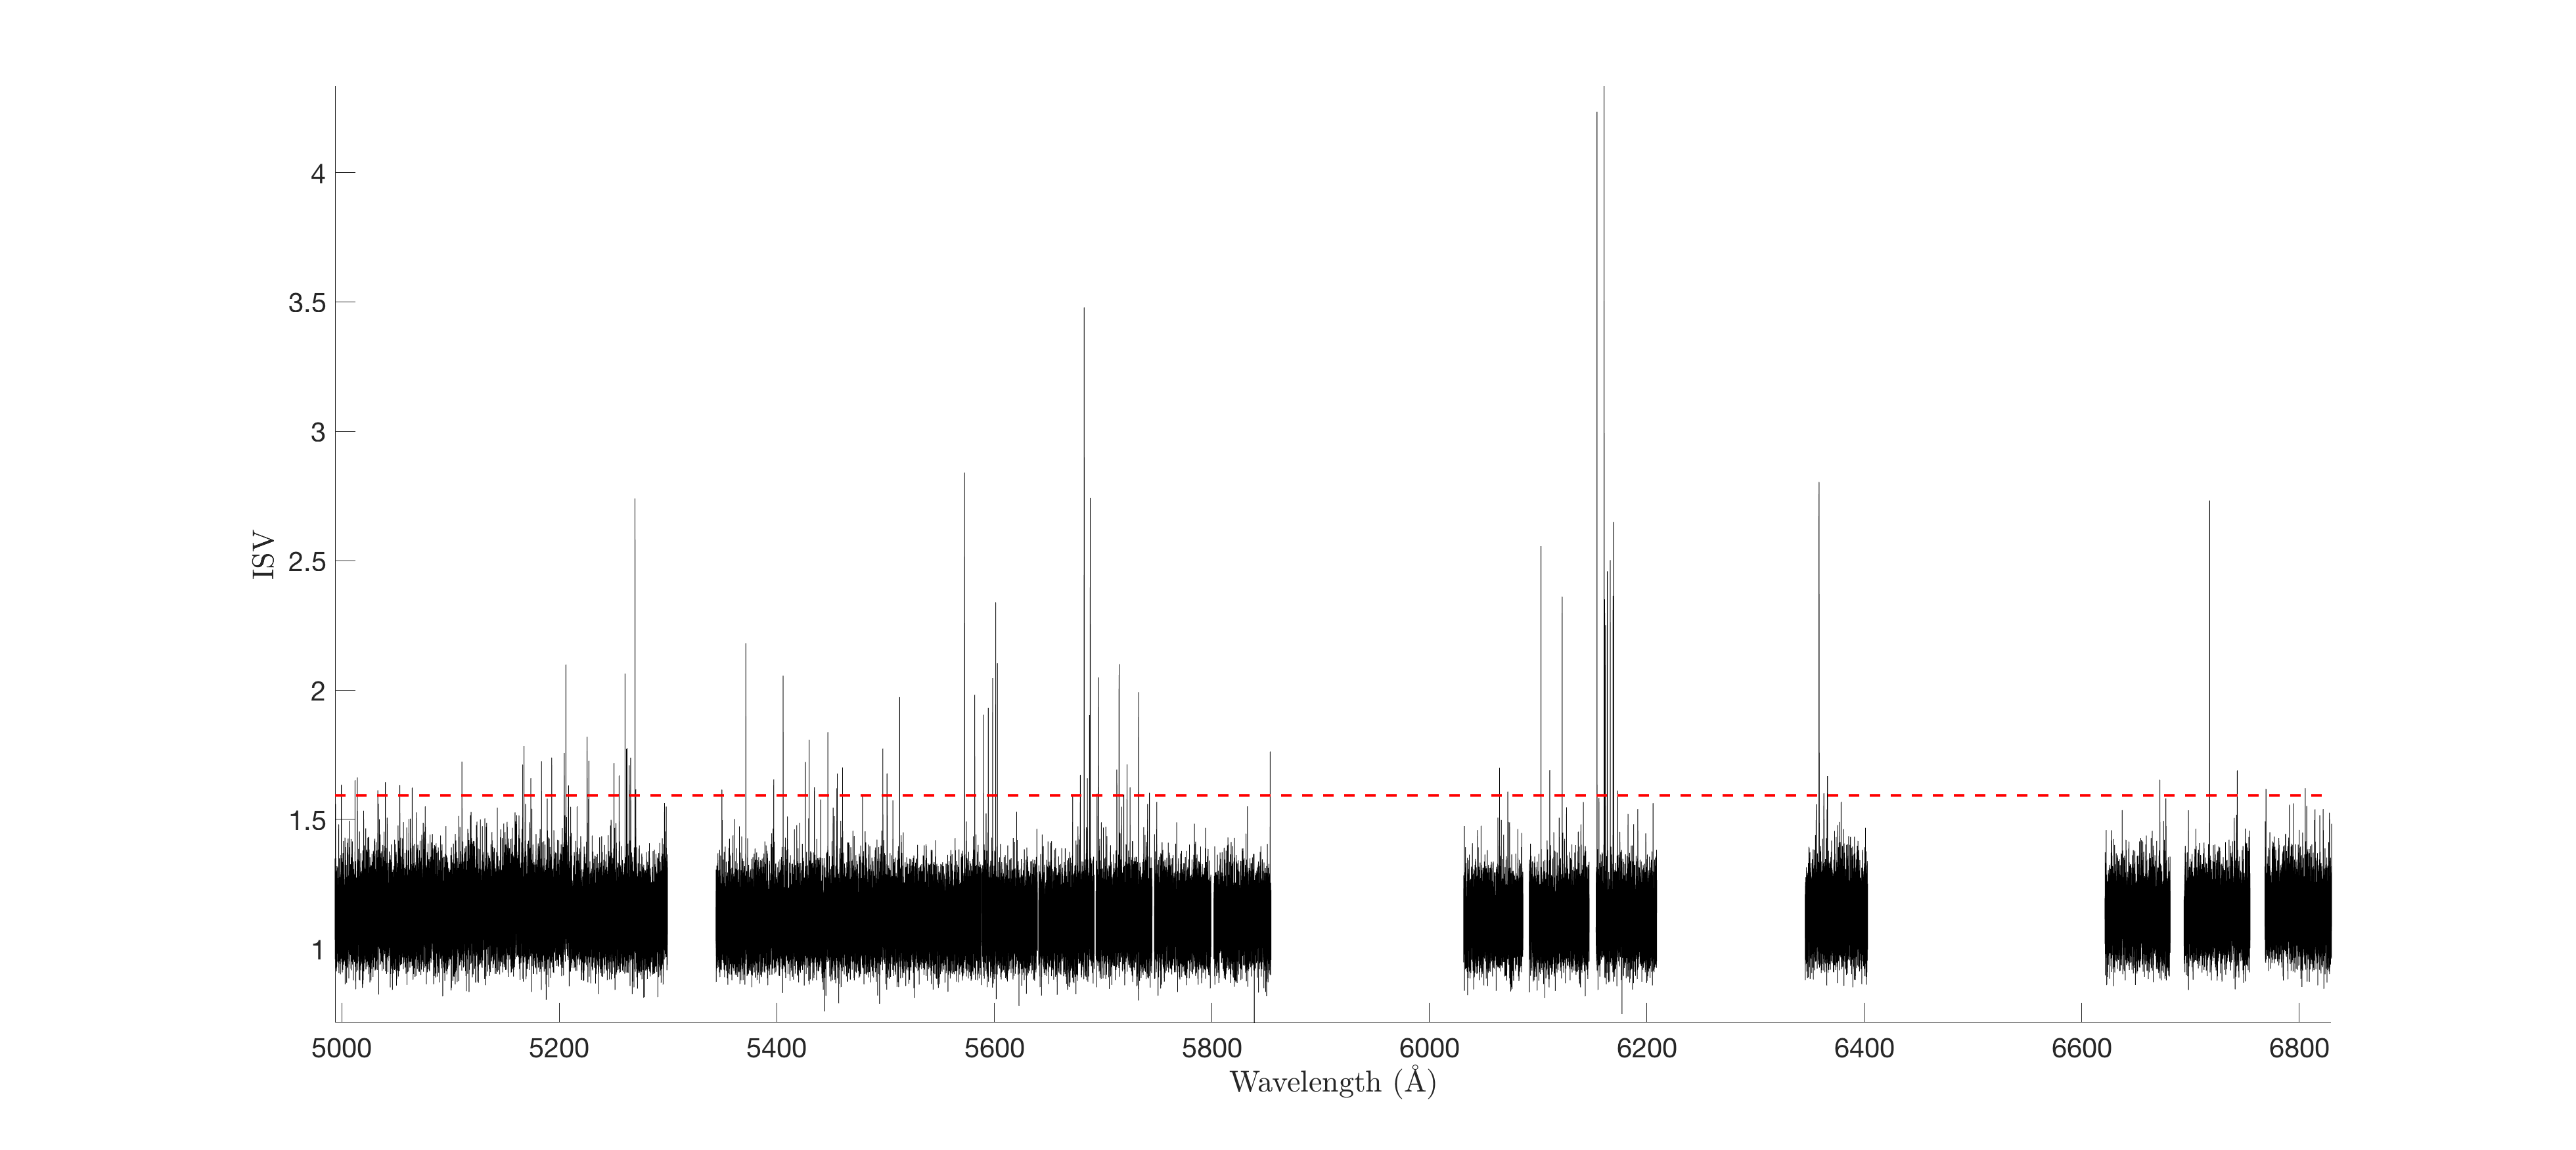
\includegraphics[width=1\textwidth]{ISVplots/thesis_Gl191.png}}\\
    \subfloat[GL205]{\label{figISV6}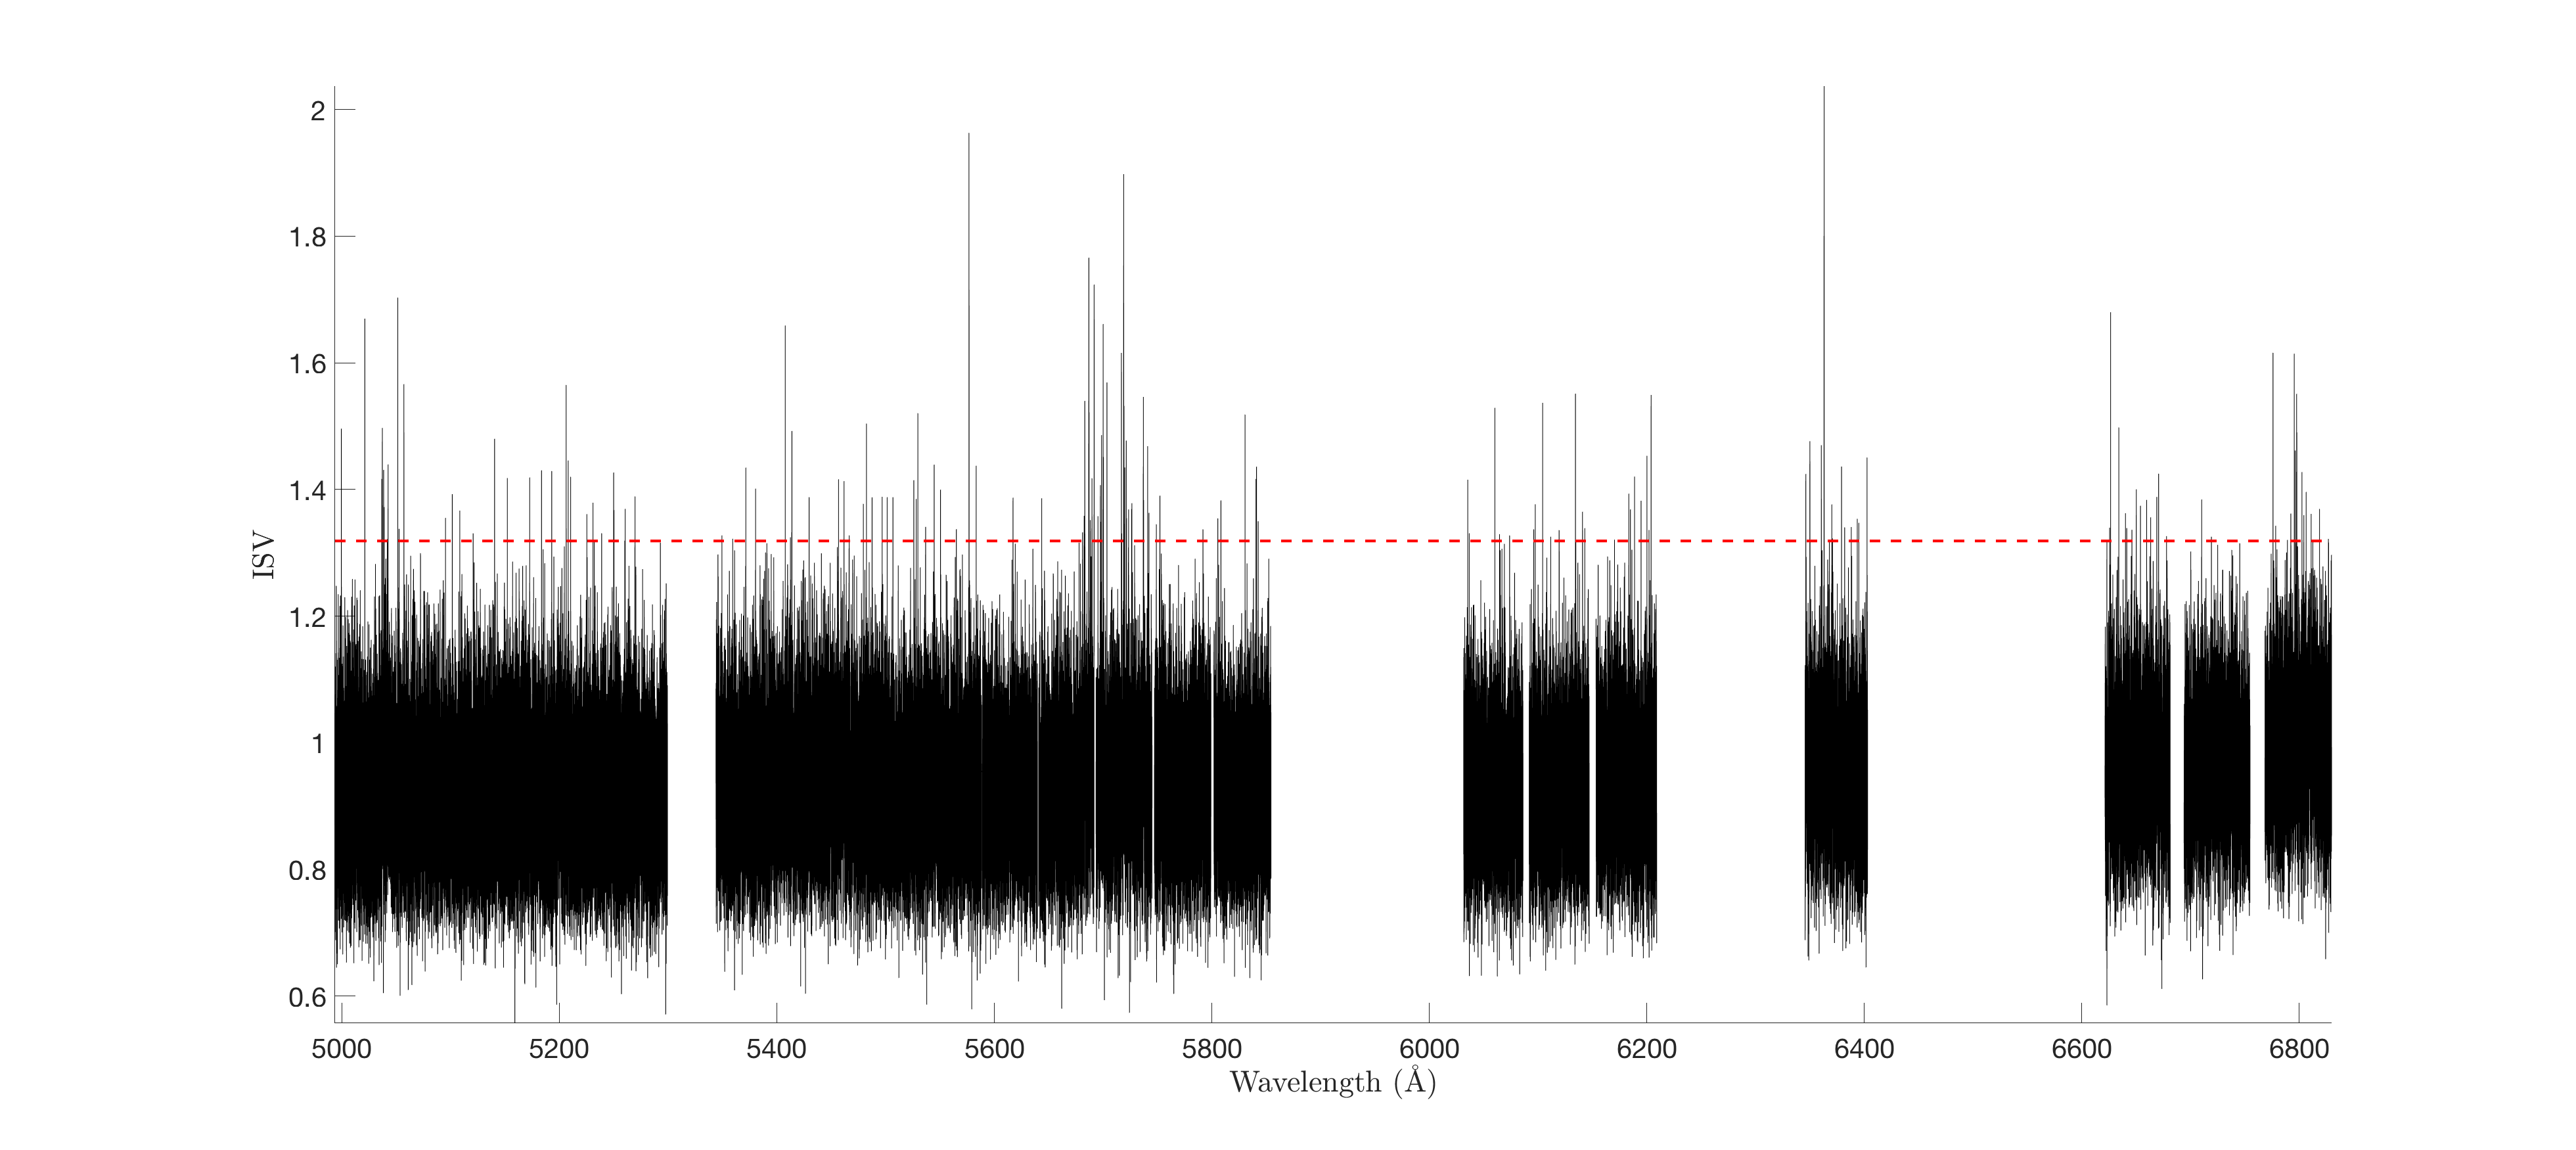
\includegraphics[width=1\textwidth]{ISVplots/thesis_Gl205.png}}
    \caption{}
\end{figure}

\begin{figure}
    \subfloat[GL213]{\label{figISV7}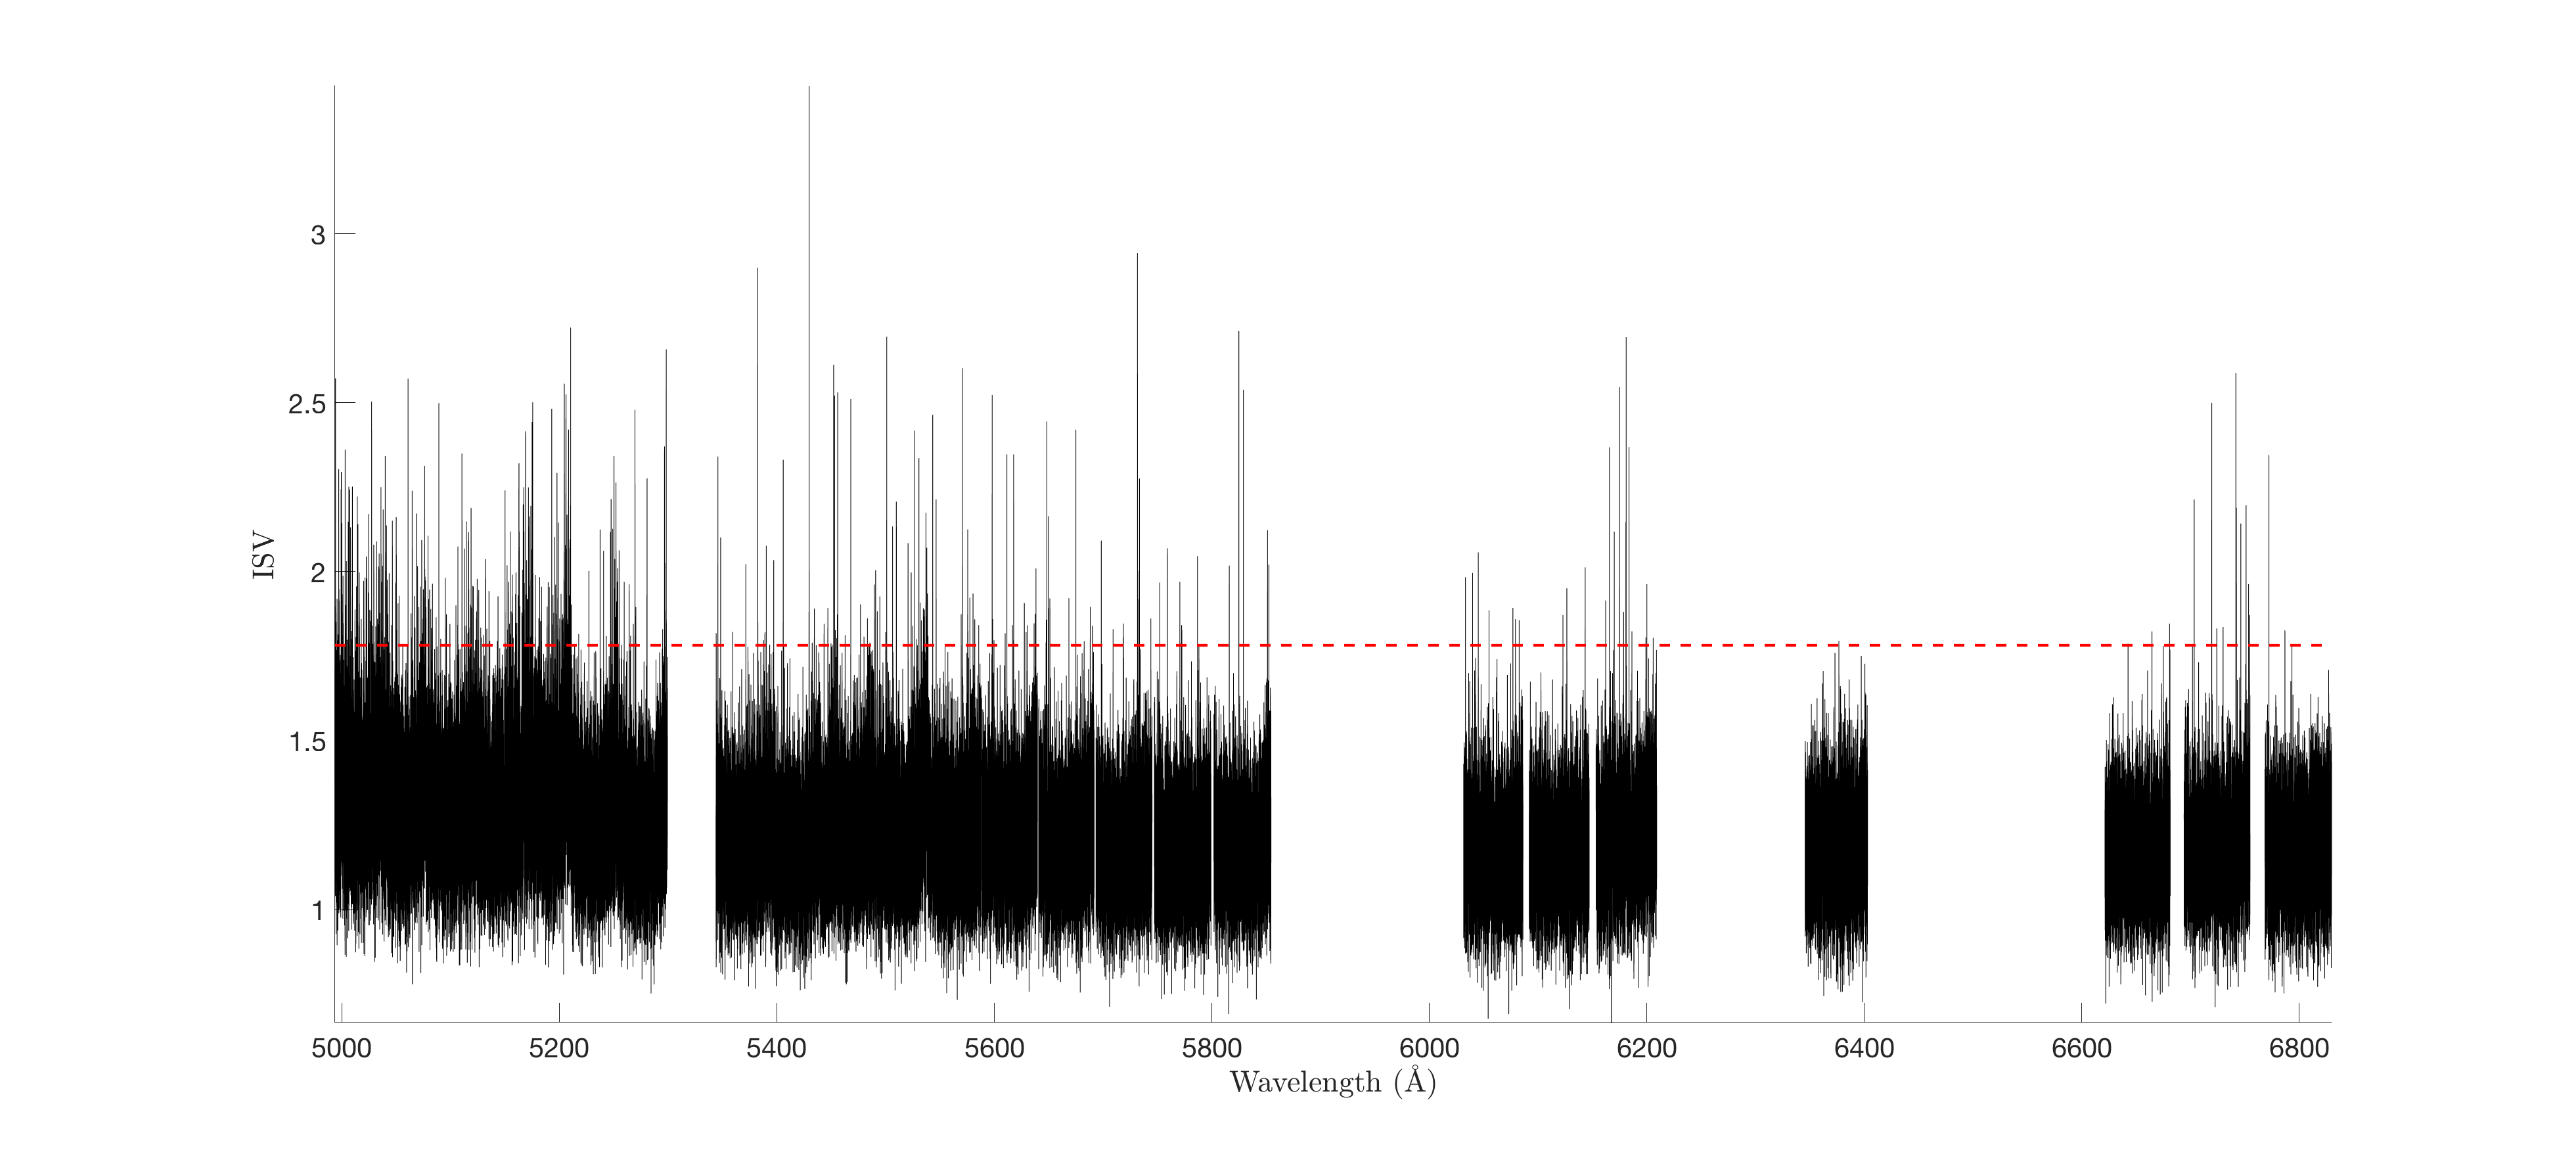
\includegraphics[width=1\textwidth]{ISVplots/thesis_Gl213.png}}\\
    \subfloat[GL229]{\label{figISV8}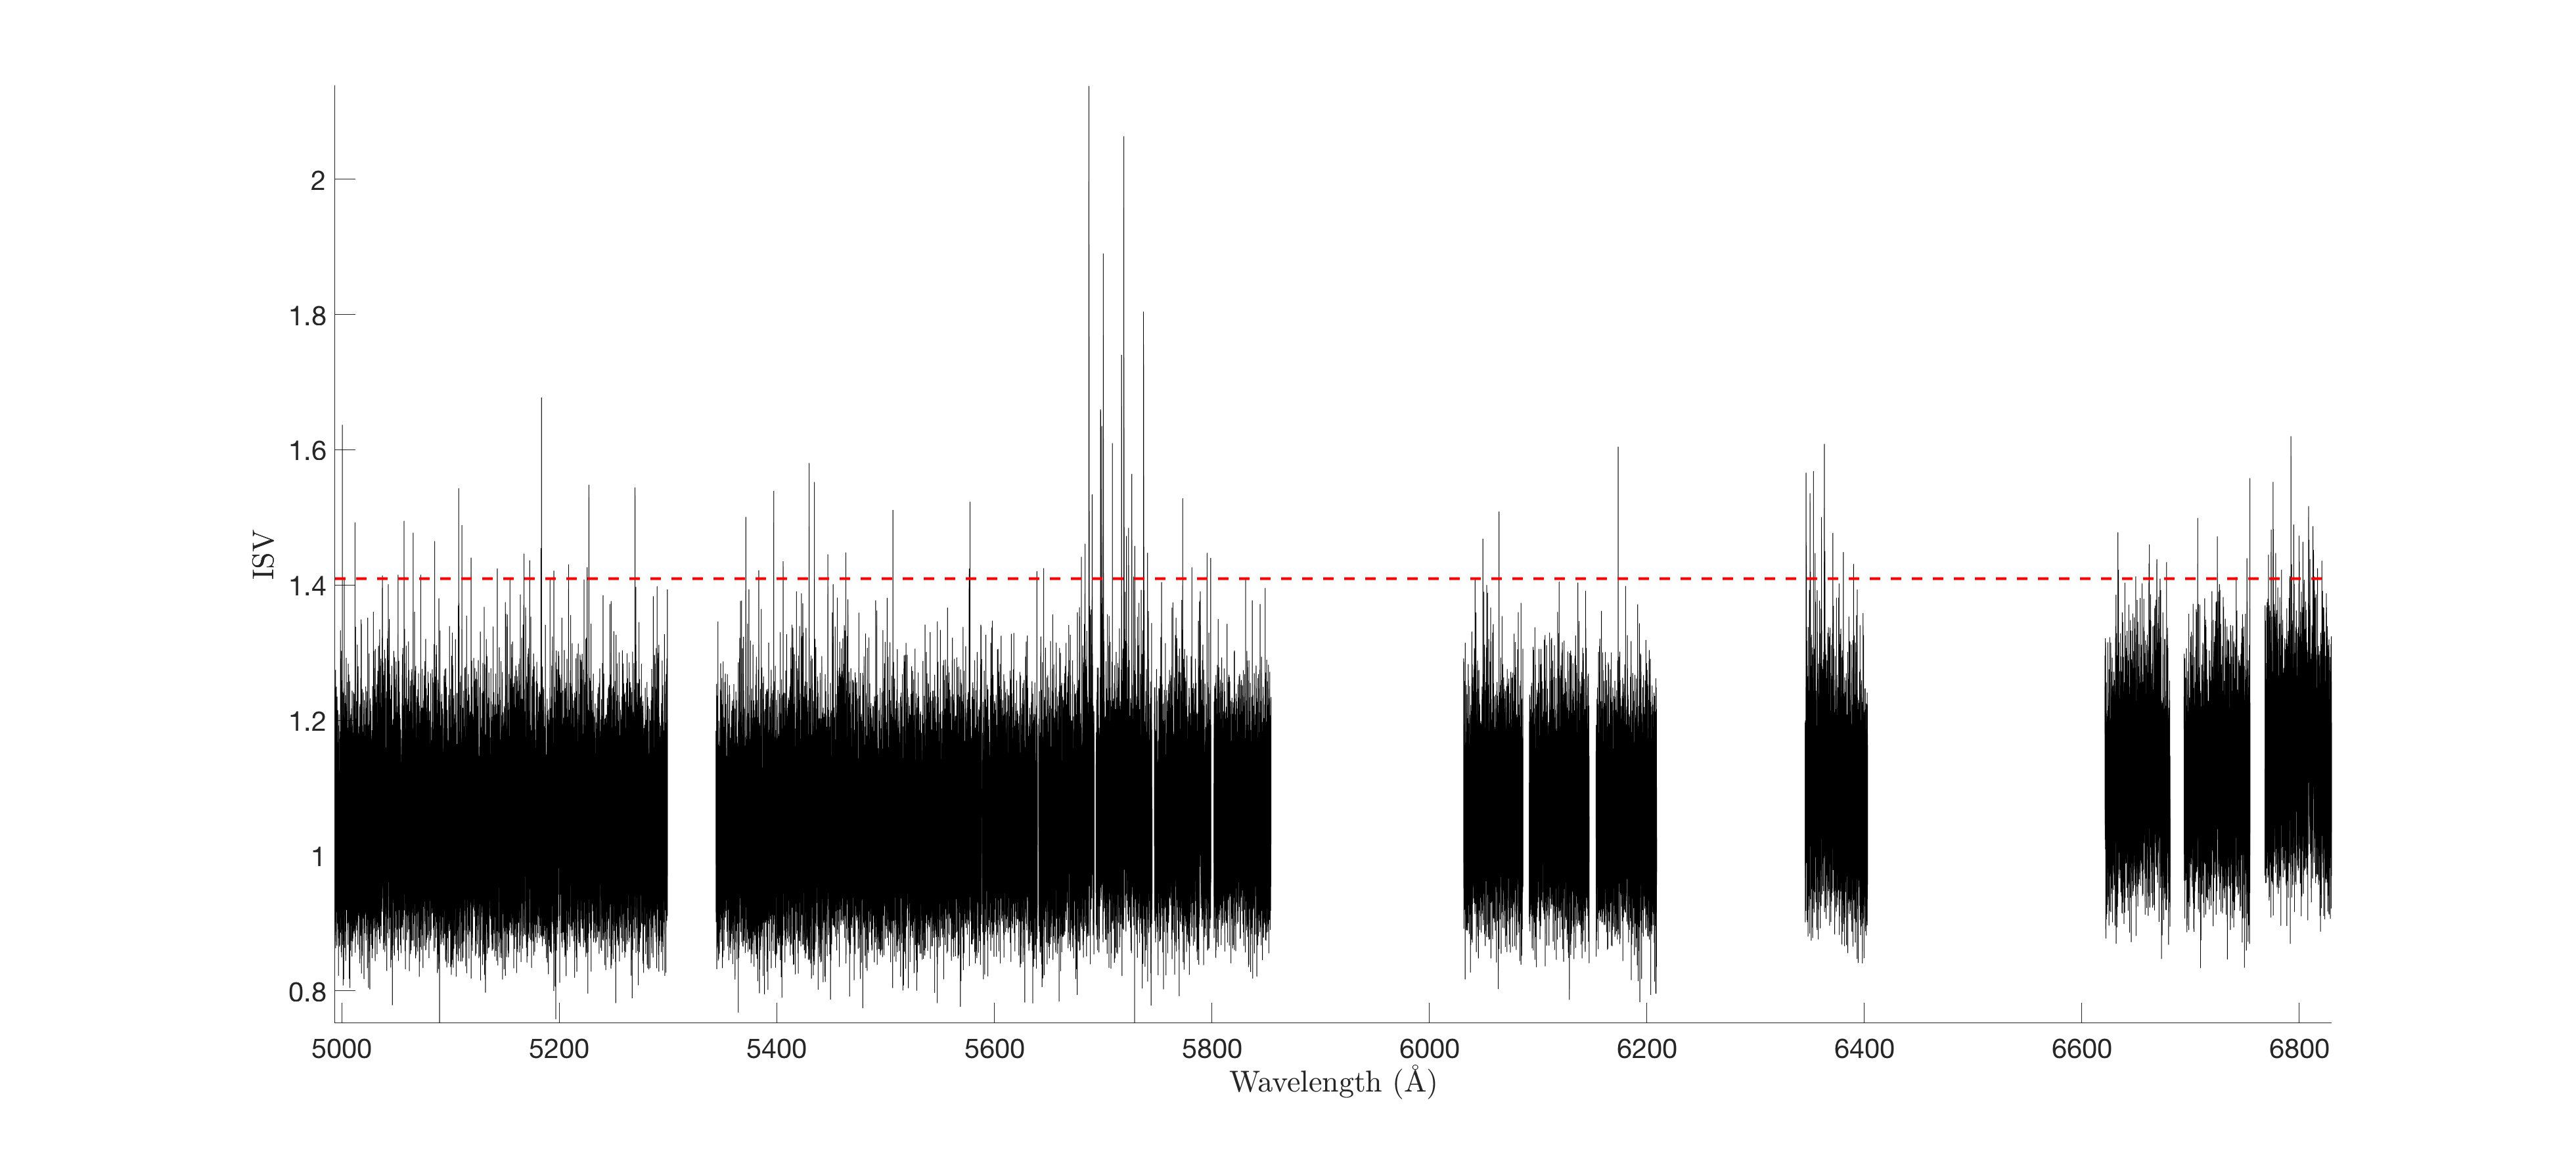
\includegraphics[width=1\textwidth]{ISVplots/thesis_Gl229.png}}\\
    \subfloat[GL273]{\label{figISV9}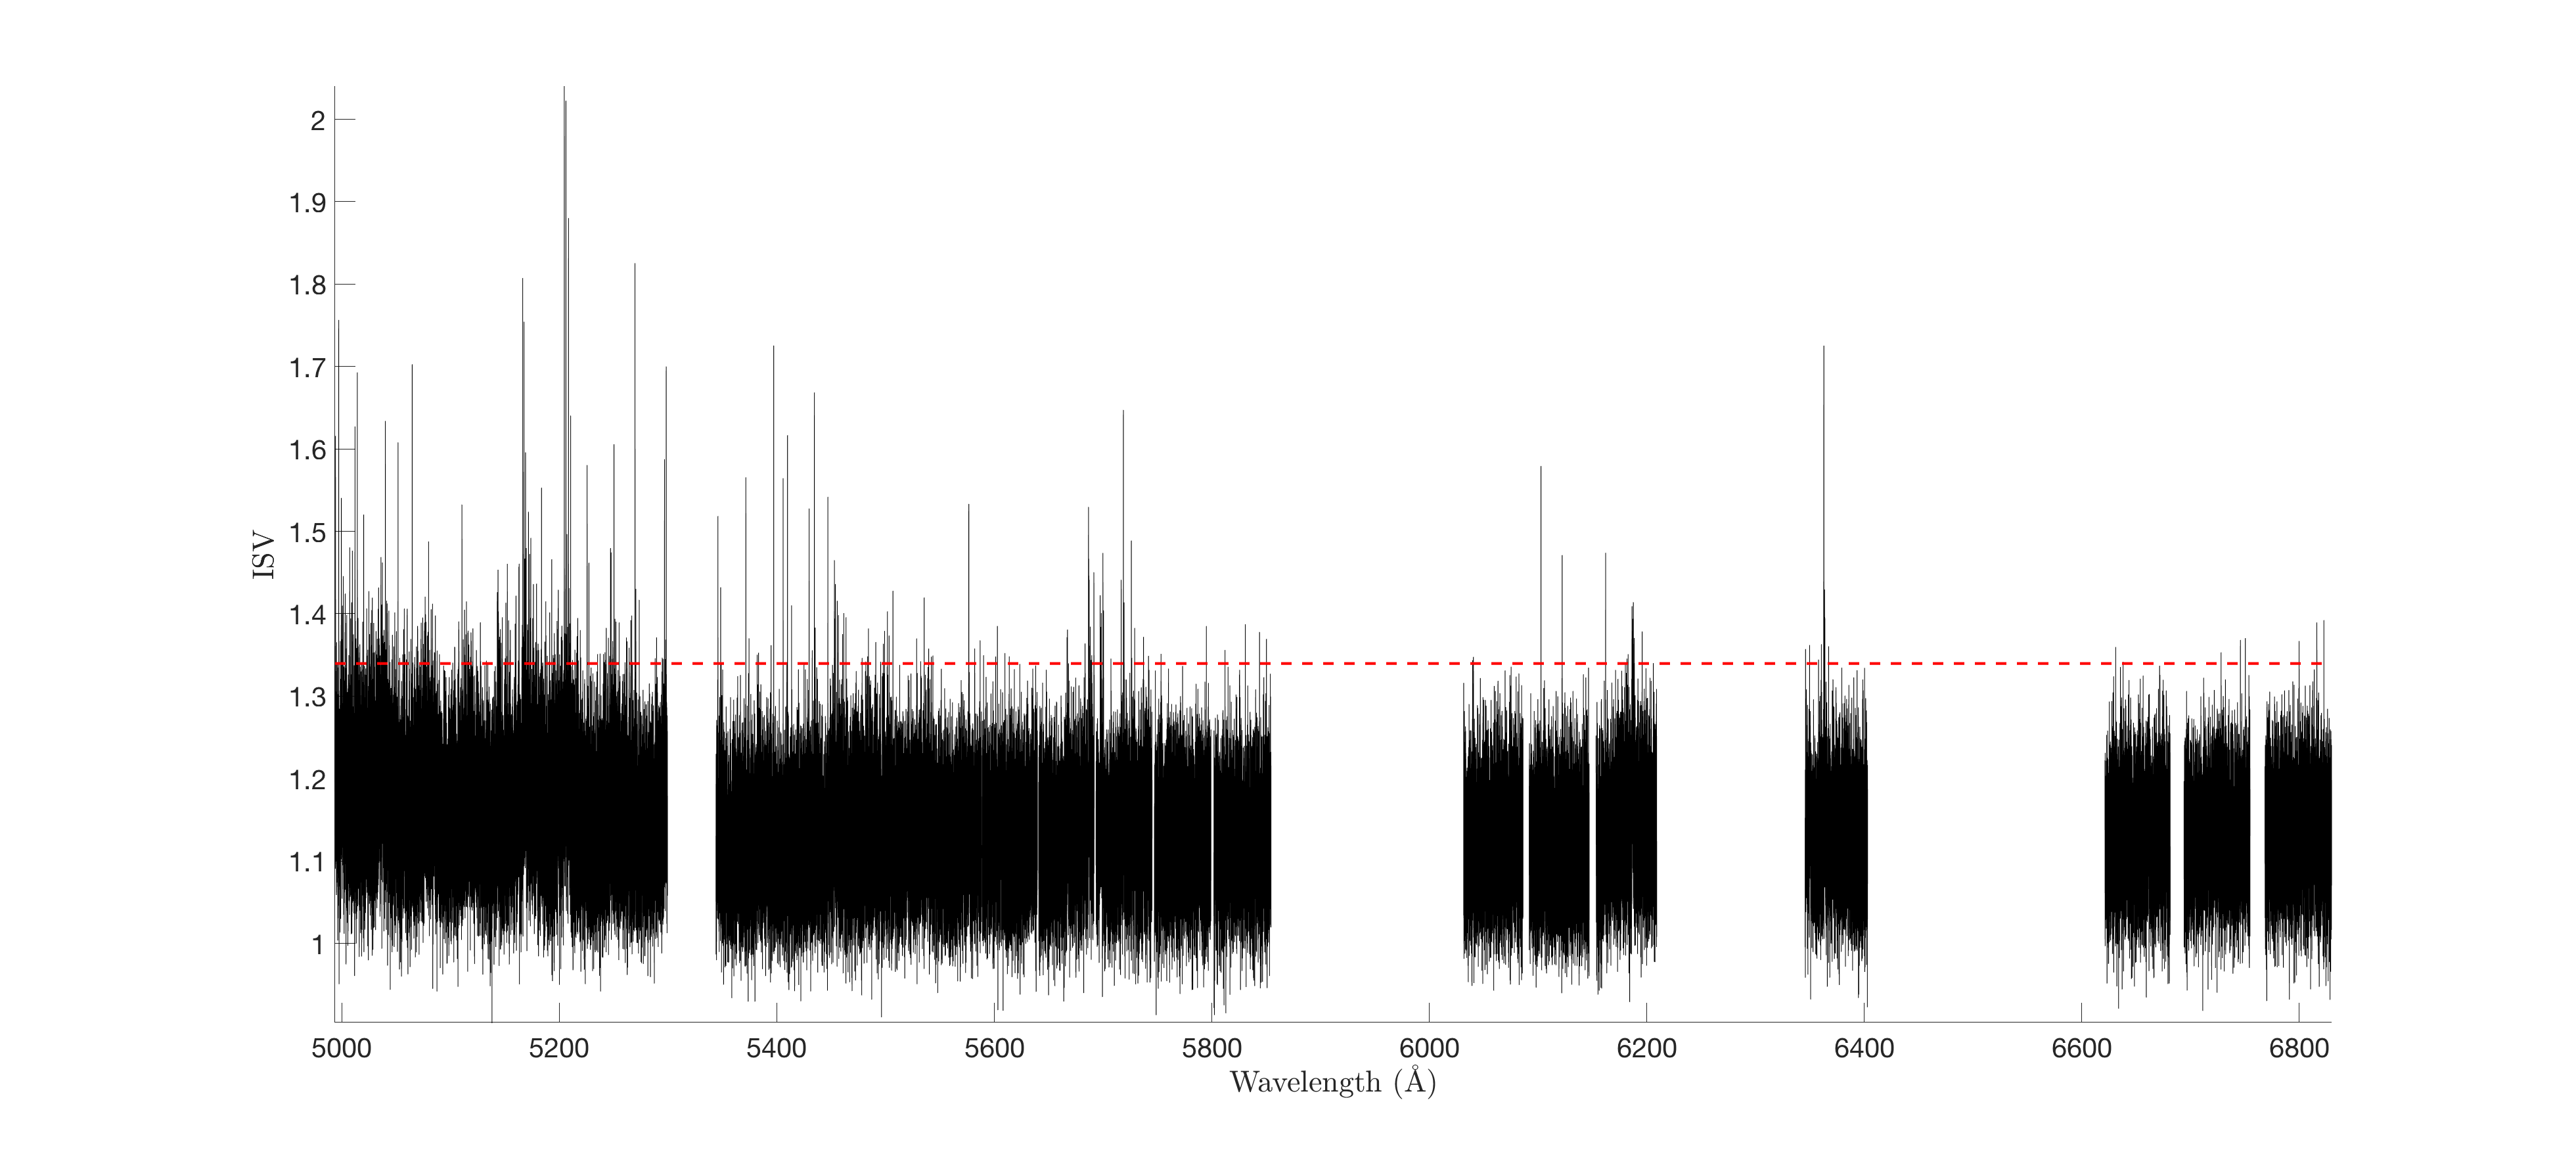
\includegraphics[width=1\textwidth]{ISVplots/thesis_Gl273.png}}
    \caption{}
\end{figure}

\begin{figure}
    \subfloat[GL299]{\label{figISV10}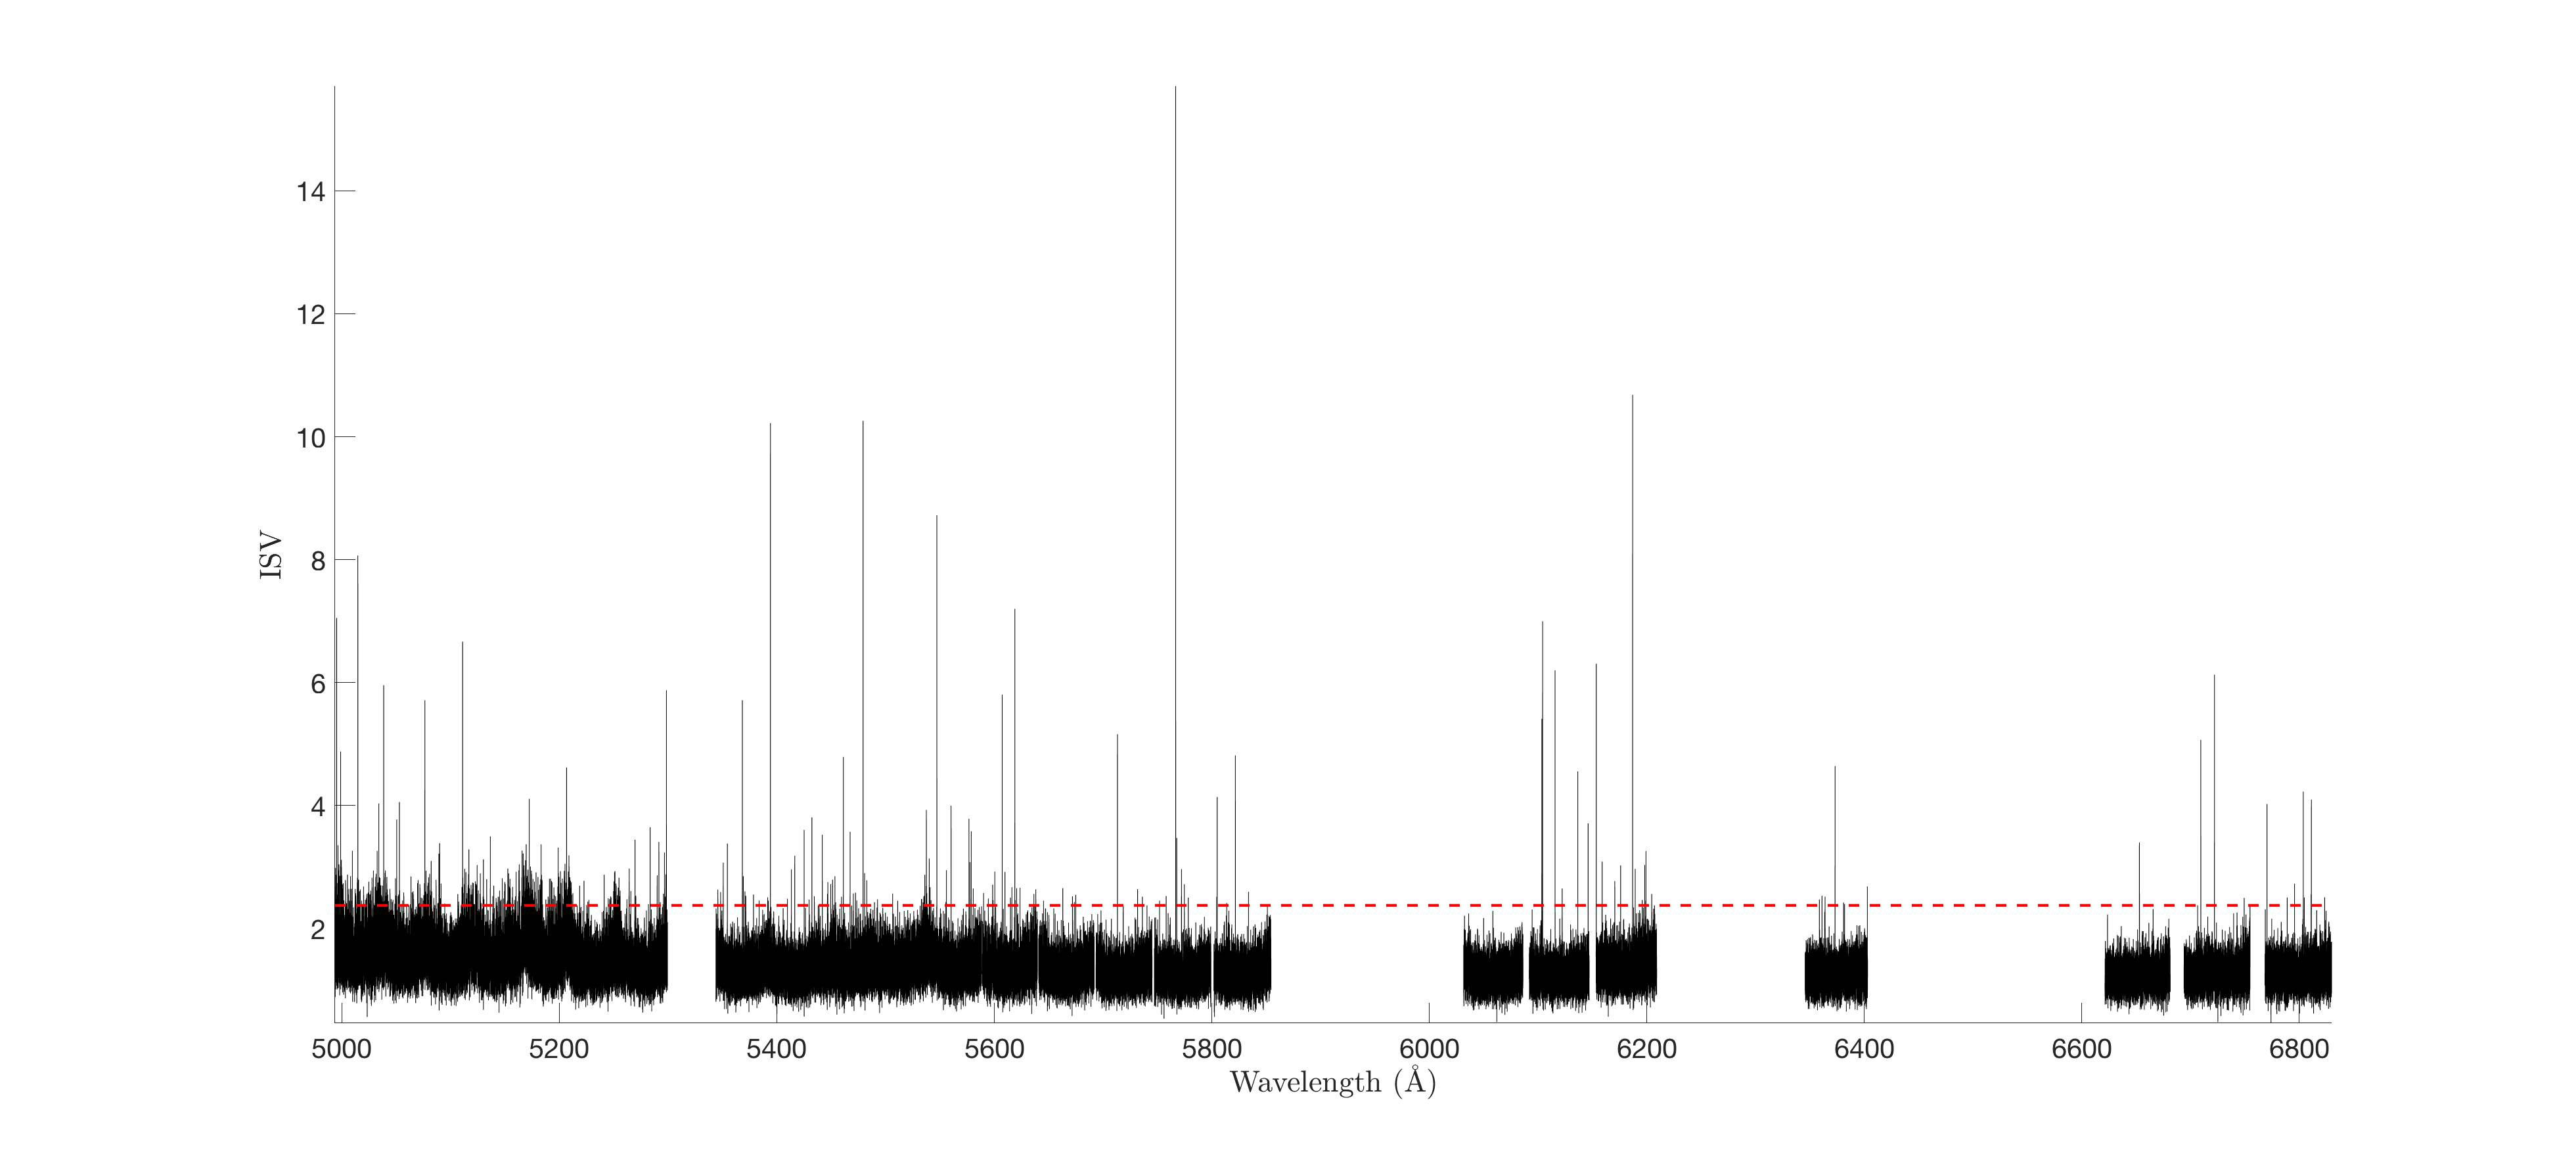
\includegraphics[width=1\textwidth]{ISVplots/thesis_Gl299.png}}\\
    \subfloat[GL300]{\label{figISV11}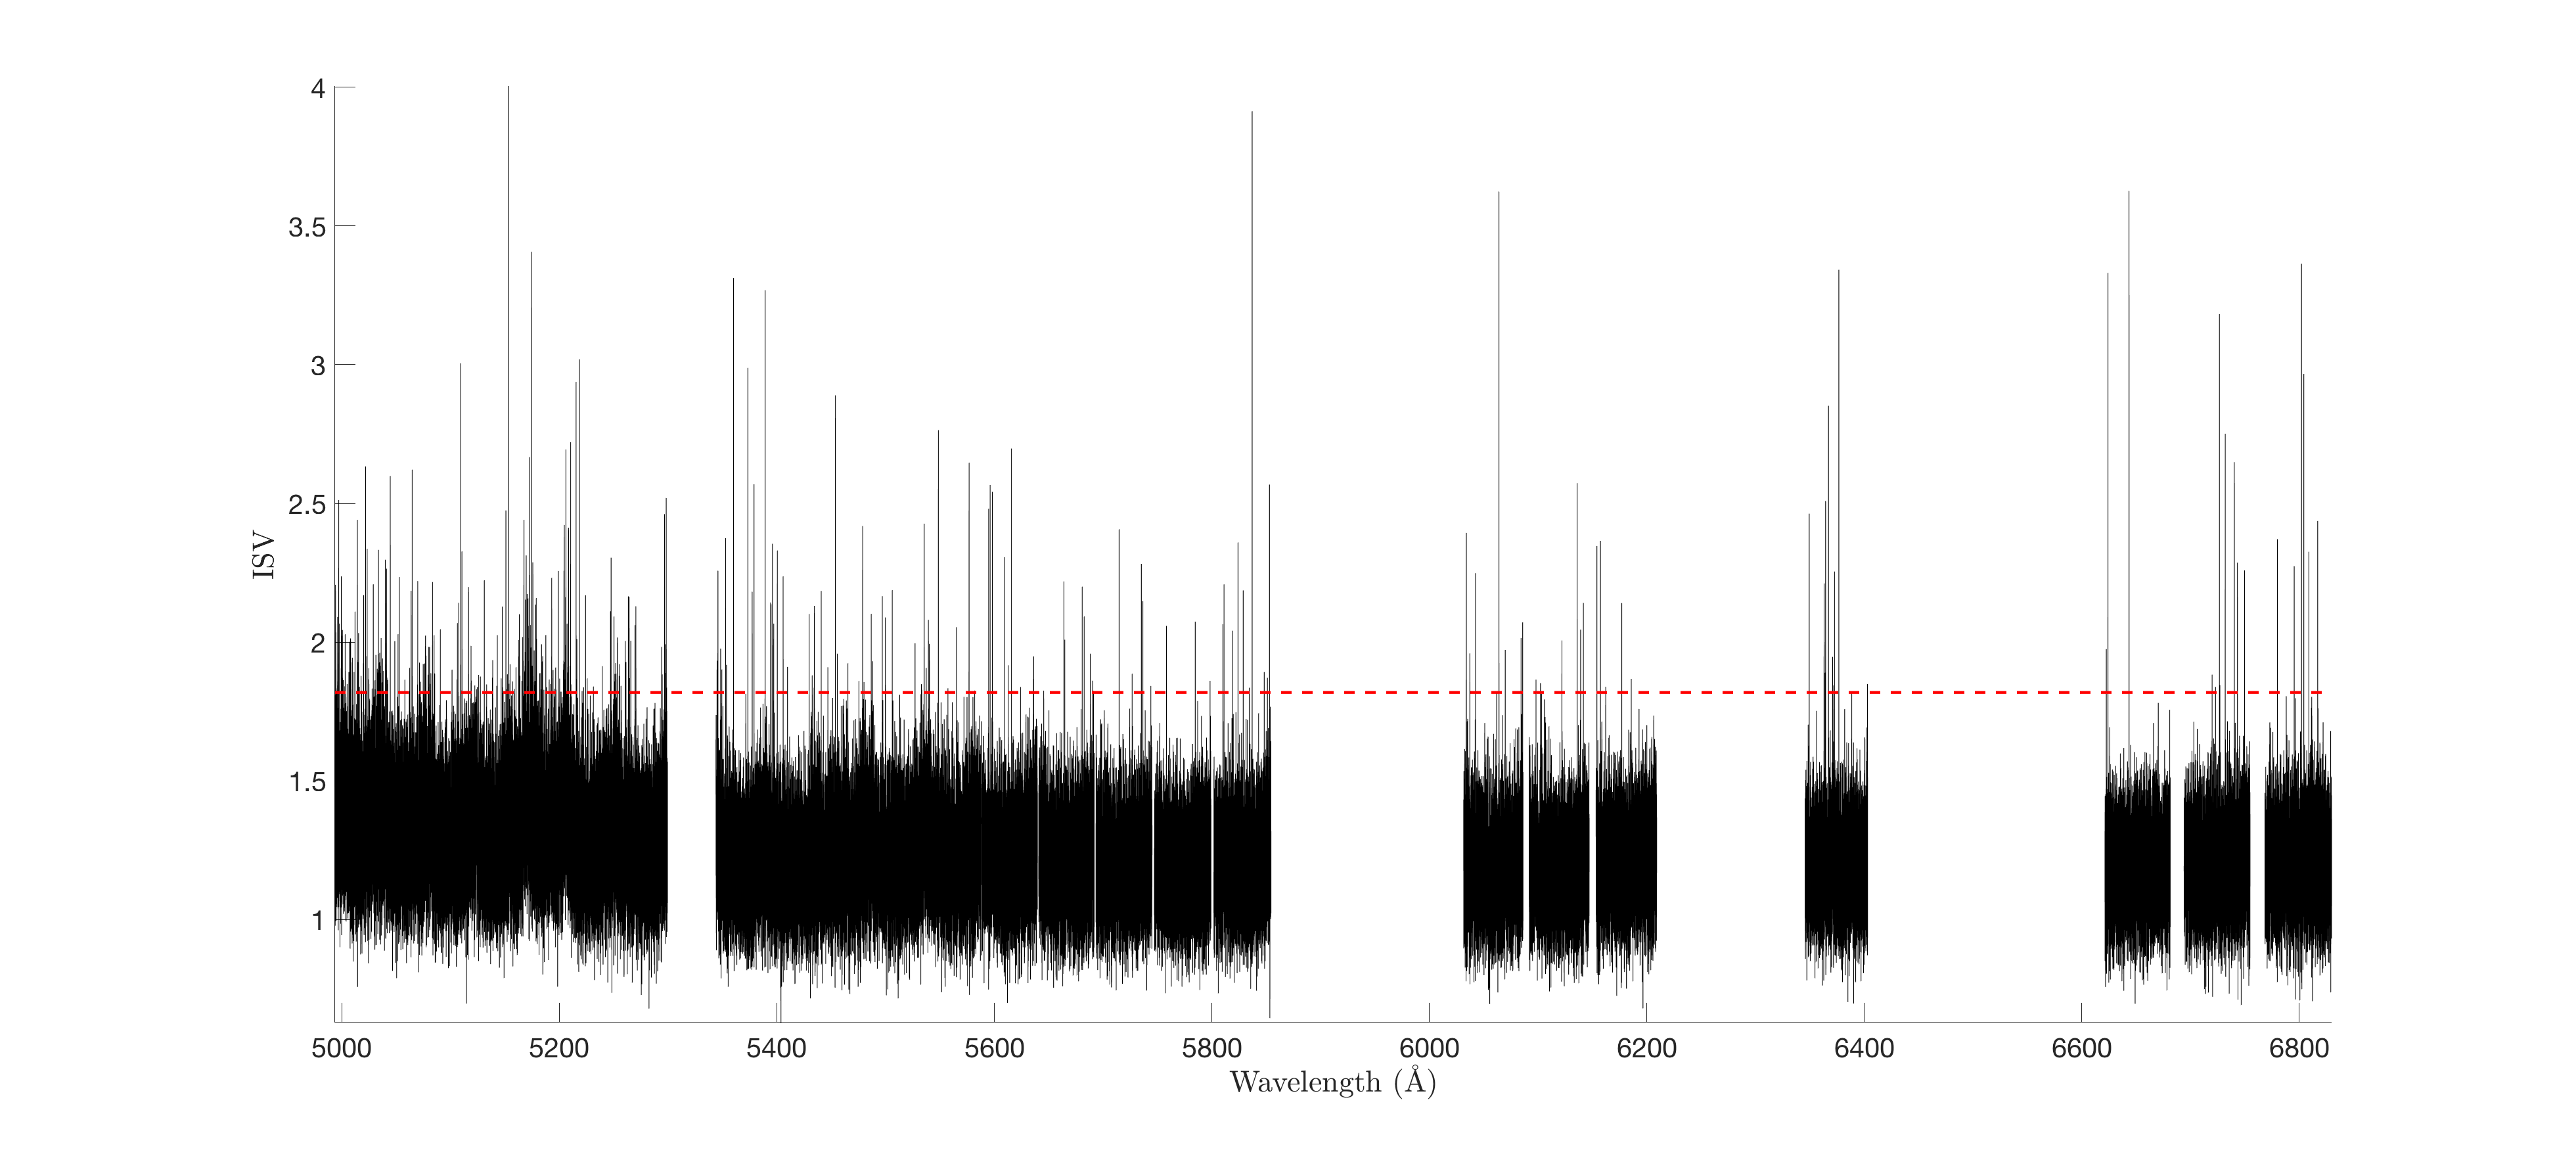
\includegraphics[width=1\textwidth]{ISVplots/thesis_Gl300.png}}\\
    \subfloat[GL341]{\label{figISV12}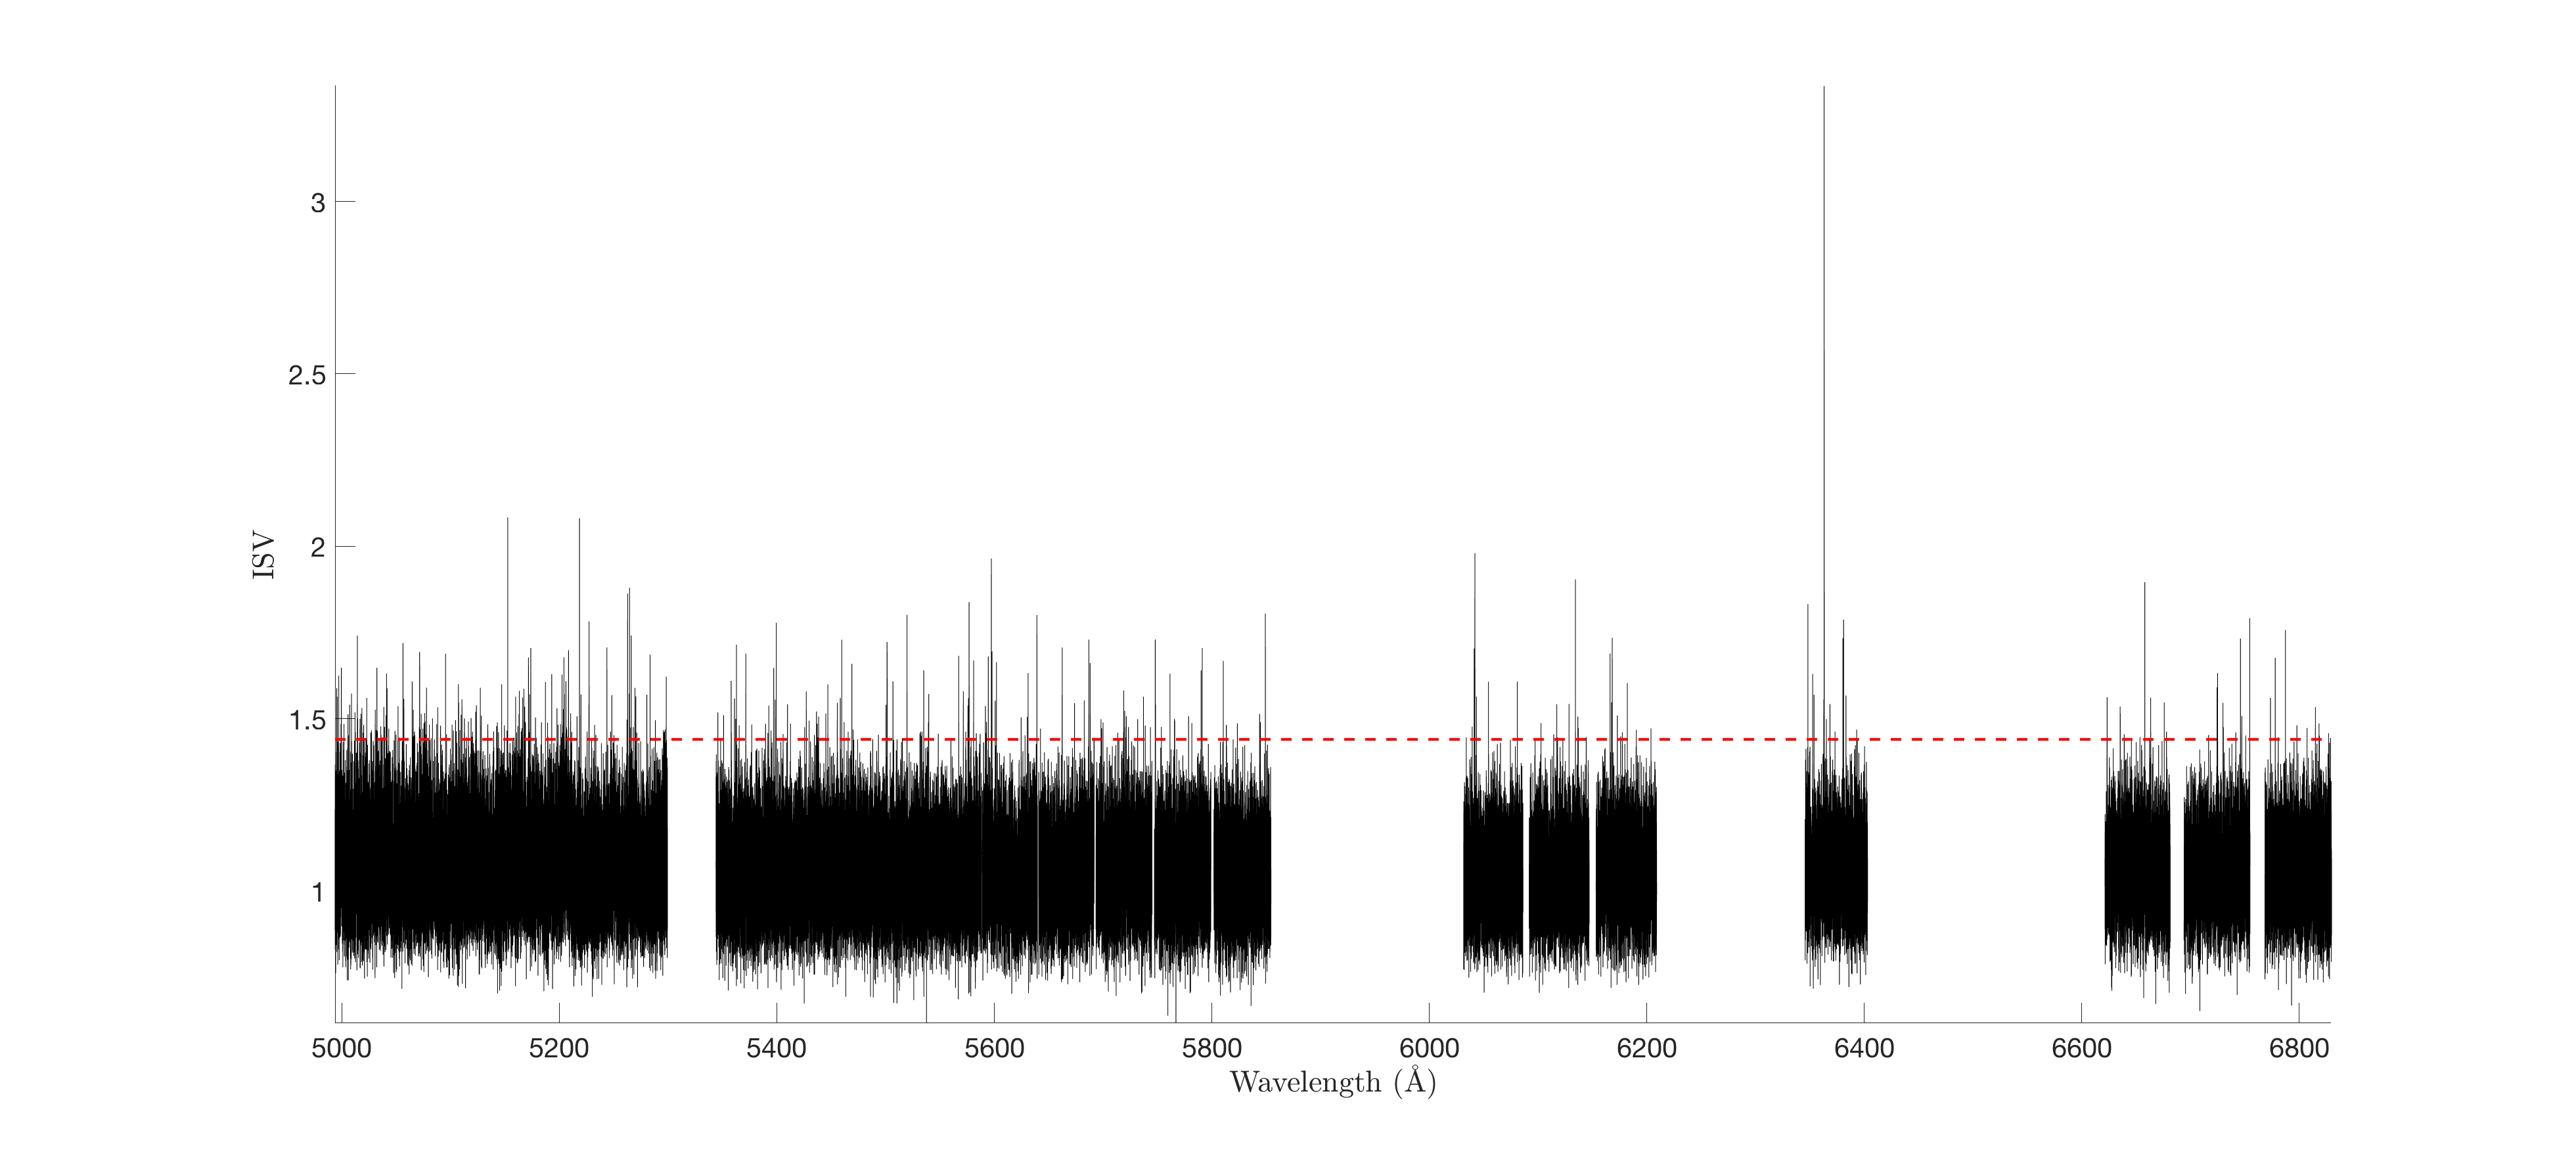
\includegraphics[width=1\textwidth]{ISVplots/thesis_Gl341.png}}
    \caption{}
\end{figure}

\begin{figure}
    \subfloat[GL357]{\label{figISV13}\includegraphics[width=1\textwidth]{ISVplots/thesis_Gl357.png}}\\
    \subfloat[GL358]{\label{figISV14}\includegraphics[width=1\textwidth]{ISVplots/thesis_Gl358.png}}\\
    \subfloat[GL367]{\label{figISV15}\includegraphics[width=1\textwidth]{ISVplots/thesis_Gl367.png}}
    \caption{}
\end{figure}

\begin{figure}
    \subfloat[GL382]{\label{figISV16}\includegraphics[width=1\textwidth]{ISVplots/thesis_Gl382.png}}\\
    \subfloat[GL388]{\label{figISV17}\includegraphics[width=1\textwidth]{ISVplots/thesis_Gl388.png}}\\
    \subfloat[GL393]{\label{figISV18}\includegraphics[width=1\textwidth]{ISVplots/thesis_Gl393.png}}
    \caption{}
\end{figure}

\begin{figure}
    \subfloat[GL433]{\label{figISV19}\includegraphics[width=1\textwidth]{ISVplots/thesis_Gl433.png}}\\
    \subfloat[GL447]{\label{figISV20}\includegraphics[width=1\textwidth]{ISVplots/thesis_Gl447.png}}\\
    \subfloat[GL465]{\label{figISV21}\includegraphics[width=1\textwidth]{ISVplots/thesis_Gl465.png}}
    \caption{}
\end{figure}

\begin{figure}
    \subfloat[GL479]{\label{figISV22}\includegraphics[width=1\textwidth]{ISVplots/thesis_Gl479.png}}\\
    \subfloat[GL514]{\label{figISV23}\includegraphics[width=1\textwidth]{ISVplots/thesis_Gl514.png}}\\
    \subfloat[GL526]{\label{figISV24}\includegraphics[width=1\textwidth]{ISVplots/thesis_Gl526.png}}
    \caption{}
\end{figure}

\begin{figure}
    \subfloat[GL536]{\label{figISV25}\includegraphics[width=1\textwidth]{ISVplots/thesis_Gl536.png}}\\
    \subfloat[GL54.1]{\label{figISV26}\includegraphics[width=1\textwidth]{ISVplots/thesis_Gl54_1.png}}\\
    \subfloat[GL551]{\label{figISV27}\includegraphics[width=1\textwidth]{ISVplots/thesis_Gl551.png}}
    \caption{}
\end{figure}

\begin{figure}
    \subfloat[GL569A]{\label{figISV28}\includegraphics[width=1\textwidth]{ISVplots/thesis_Gl569A.png}}\\
    \subfloat[GL581]{\label{figISV29}\includegraphics[width=1\textwidth]{ISVplots/thesis_Gl581.png}}\\
    \subfloat[GL588]{\label{figISV30}\includegraphics[width=1\textwidth]{ISVplots/thesis_Gl588.png}}
    \caption{}
\end{figure}

\begin{figure}
    \subfloat[GL618A]{\label{figISV31}\includegraphics[width=1\textwidth]{ISVplots/thesis_Gl618A.png}}\\
    \subfloat[GL628]{\label{figISV32}\includegraphics[width=1\textwidth]{ISVplots/thesis_Gl628.png}}\\
    \subfloat[GL667C]{\label{figISV33}\includegraphics[width=1\textwidth]{ISVplots/thesis_Gl667C.png}}
    \caption{}
\end{figure}

\begin{figure}
    \subfloat[GL674]{\label{figISV34}\includegraphics[width=1\textwidth]{ISVplots/thesis_Gl674.png}}\\
    \subfloat[GL678.1A]{\label{figISV35}\includegraphics[width=1\textwidth]{ISVplots/thesis_Gl678_1A.png}}\\
    \subfloat[GL680]{\label{figISV36}\includegraphics[width=1\textwidth]{ISVplots/thesis_Gl680.png}}
    \caption{}
\end{figure}

\begin{figure}
    \subfloat[GL682]{\label{figISV37}\includegraphics[width=1\textwidth]{ISVplots/thesis_Gl682.png}}\\
    \subfloat[GL686]{\label{figISV38}\includegraphics[width=1\textwidth]{ISVplots/thesis_Gl686.png}}\\
    \subfloat[GL693]{\label{figISV39}\includegraphics[width=1\textwidth]{ISVplots/thesis_Gl693.png}}
    \caption{}
\end{figure}

\begin{figure}
    \subfloat[GL699]{\label{figISV40}\includegraphics[width=1\textwidth]{ISVplots/thesis_Gl699.png}}\\
    \subfloat[GL701]{\label{figISV41}\includegraphics[width=1\textwidth]{ISVplots/thesis_Gl701.png}}\\
    \subfloat[GL752A]{\label{figISV42}\includegraphics[width=1\textwidth]{ISVplots/thesis_Gl752A.png}}
    \caption{}
\end{figure}

\begin{figure}
    \subfloat[GL754]{\label{figISV43}\includegraphics[width=1\textwidth]{ISVplots/thesis_Gl754.png}}\\
    \subfloat[GL832]{\label{figISV44}\includegraphics[width=1\textwidth]{ISVplots/thesis_Gl832.png}}\\
    \subfloat[GL849]{\label{figISV45}\includegraphics[width=1\textwidth]{ISVplots/thesis_Gl849.png}}
    \caption{}
\end{figure}

\begin{figure}
    \subfloat[GL87]{\label{figISV46}\includegraphics[width=1\textwidth]{ISVplots/thesis_Gl87.png}}\\
    \subfloat[GL908]{\label{figISV47}\includegraphics[width=1\textwidth]{ISVplots/thesis_Gl908.png}}\\
    \subfloat[HIP85647]{\label{figISV48}\includegraphics[width=1\textwidth]{ISVplots/thesis_HIP85647.png}}
    \caption{}
\end{figure}

\begin{figure}
    \subfloat[LHS1723]{\label{figISV49}\includegraphics[width=1\textwidth]{ISVplots/thesis_LHS1723.png}}
    \caption{}
\end{figure}

\subsection{Frequently varying stellar lines}
\begin{longtable}{|c|c|c|c|c|}
    \hline
    Element & $\lambda$ (\AA) & P$_{CaHK}$ & P$_{H\alpha}$ & P$_{NaD}$\\
    \hline
    \endfirsthead
    
    \hline
    Element & $\lambda$ (\AA) & P$_{CaHK}$ & P$_{H\alpha}$ & P$_{NaD}$\\
    \hline
    \endhead
    
    \hline
    \endfoot
    
    \endlastfoot
Fe 1 & 4994.130 & 0.67608 & 0.76544 & 0.21625 \\   
Ti 1 & 4997.097 & 0.51575 & 0.58566 & 0.38929 \\  
Ti 1 & 4999.503 & 0.49467 & 0.61319 & 0.070795 \\ 
Ti 1 & 5007.209 & 0.22817 & 0.31188 & -0.018478 \\
Fe 1 & 5012.068 & 0.87570 & 0.89865 & 0.62873 \\   
Ti 1 & 5020.026 & 0.37678 & 0.44476 & 0.1798 \\   
Ti 1 & 5024.844 & 0.74216 & 0.80768 & -0.037137 \\
Ti 1 & 5039.957 & 0.62210 & 0.72223 & 0.10316 \\   
Fe 1 & 5041.072 & 0.83354 & 0.89161 & 0.54918 \\  
Fe 1 & 5051.635 & 0.68952 & 0.68182 & 0.40891 \\  
Ti 1 & 5064.653 & 0.34410 & 0.30567 & 0.050078 \\  
Fe 1 & 5083.339 & 0.54992 & 0.53720 & 0.39208 \\   
Fe 1 & 5110.413 & 0.89007 & 0.79586 & 0.56134 \\  
Fe 1 & 5166.282 & 0.74465 & 0.76435 & 0.54544 \\  
Fe 1 & 5171.596 & 0.58926 & 0.51301 & 0.64234 \\  
Mg 1 & 5172.684 & 0.64768 & 0.87064 & 0.54545 \\  
Ti 1 & 5173.743 & 0.75220 & 0.77750 & 0.52413 \\    
Mg 1 & 5183.604 & 0.63769 & 0.86673 & 0.55056 \\  
Ti 1 & 5192.969 & 0.77547 & 0.81554 & 0.53267 \\  
Cr 1 & 5206.023 & 0.49595 & 0.60226 & 0.059784 \\ 
Ti 1 & 5210.384 & 0.38605 & 0.50458 & -0.081414 \\
Fe 1 & 5227.190 & 0.61175 & 0.87405 & 0.53314 \\   
Cr 1 & 5247.565 & 0.48422 & 0.55447 & 0.22932 \\  
Fe 1 & 5269.537 & 0.68906 & 0.88567 & 0.51604 \\  
Cr 1 & 5296.691 & 0.72230 & 0.77263 & 0.56689 \\   
Cr 1 & 5298.272 & 0.61489 & 0.71844 & 0.17098 \\  
Cr 1 & 5345.796 & 0.55845 & 0.59737 & 0.24659 \\  
Cr 1 & 5348.314 & 0.45584 & 0.46596 & 0.2535 \\   
Fe 1 & 5371.489 & 0.65591 & 0.88131 & 0.56698 \\  
Fe 1 & 5397.128 & 0.63076 & 0.84673 & 0.44517 \\  
Fe 1 & 5405.775 & 0.68726 & 0.91068 & 0.55559 \\  
Cr 1 & 5409.783 & 0.69079 & 0.89872 & 0.65042 \\  
Fe 1 & 5429.696 & 0.68492 & 0.90272 & 0.51864 \\  
Fe 1 & 5434.524 & 0.74452 & 0.86759 & 0.56037 \\  
Fe 1 & 5506.779 & 0.67394 & 0.66560 & 0.40797 \\   
Ca 1 & 6122.217 & 0.88710 & 0.92345 & 0.65719 \\   
Ca 1 & 6162.173 & 0.81981 & 0.91452 & 0.75695 \\ 
\hline
\caption{Stellar lines found to be variable in ten or more stars in the HARPS M-dwarf subsample. The Pearson correlations are between $A_{ISV}$ and each of the Ca\,\textsc{ii} H \& K, H\,\textsc{$\alpha$}, and Na\,\textsc{i} D S-indices.}
\label{tabISVlines}
\end{longtable}

\subsection{Impact on radial velocity precision}
Ca\,\textsc{ii} H \& K, H\,\textsc{$\alpha$}, and Na\,\textsc{i} D are useful as proxies of activity, but are also excluded from radial velocity measurements because of their intrinsic variability. Likewise, including the ISV identified varying spectral lines in the measurement of radial velocity could introduce line asymmetries that would contribute to radial velocity jitter. If their influence is significant, removal of these wavelengths could improve the precision of velocity measurements. At the same time, the removal of these lines would also reduce the number of data points used in the cross-correlation, which would act to reduce precision. These two impacts needed to be balanced. A further investigation of both the removal of all lines found to be varying (Table\,\ref{tabElementFull}; hereafter ``Full ISV'') and the subsample found to be active in 10 or more stars (Table\,\ref{tabISVlines}; hereafter ``Selected ISV'') was performed.

\subsubsection{Cross-correlation via line mask and determination of the radial velocity}
To evaluate the impact of the removal of the lines presented in Table\,\ref{tabISVlines} on velocity precision, radial velocities for each observation of each star were measured using a line mask, as mentioned in Section\,\ref{secRVanalysis}, as the template for the cross-correlation. This line mask was built from a spectrum of an M-dwarf from the sample, and contains non-zero points at the wavelength of each line in the spectrum. The magnitude of the line points are proportional to the relative strength of the lines. Cross-correlating this line mask with a spectrum excludes all wavelengths in the line mask set to zero. The wavelengths associated with the ISV spectral lines can then simply be set to zero in the template, which in turn would exclude them from the cross-correlation.\\ 

\begin{figure}[!h]
    \centering
	\captionsetup{width=.8\textwidth}
    \subfloat[Mean normalised spectrum of GL433. A pseudo-continuum (red dashed line) has been determined as the maximum flux plus an offset of 0.1. The spectral line peaks in the spectra are overplotted as black points. Examples of the lines included in the line mask are plotted as the vertical red lines. ]{\label{figlinemask1}\includegraphics[width=0.8\textwidth]{Binary_mask2.png}}\\
    \subfloat[Example line mask used to isolate the varying spectral lines identified by ISV analysis.]{\label{figlinemask2}\includegraphics[width=0.8\textwidth]{Binary_mask.png}}
    \caption{}
    \label{figlinemask}
\end{figure}

GL433 was selected as the template with which to correlate all the stars in the sample as it is bright (V\,=\,9.81), and has a large number of observations (86). As the subclasses of the M-dwarf subsample range from M0-M5.5, using an M2 star will suitably represent the average profile of all the M-dwarfs in the subsample. The mean normalised spectrum of GL433 was divided by the HARPS blaze function to remove the general profile of the order. To obtain the strength of each spectral line present, a continuum needed to be determined. As mentioned in Section\,\ref{secMdwarfs}, the M-dwarf continuum is difficult to parameterise due to the extensive molecular bands present. It would not be unreasonable to assume it would lie close to the maximum flux in the order (assuming the spectrum is free of cosmic rays). The simplest solution was to normalise each order of the de-blazed spectrum to the maximum flux in that order, plus a small offset. This produced a pseudo-continuum at a y-axis of 1 (red dashed line in Figure\,\ref{figlinemask1}) and the relative strength of a line would be the ratio between the pseudo-continuum and the normalised spectrum (the black points in Figure\,\ref{figlinemask1}). Some spectral lines will fall too close to the edge of the order and produce issues with the cross-correlation. To avoid this, the first and last thirty data points of each line mask were set to zero. This corresponded to a maximum of 0.2\,\hbox{\AA}, meaning very little information is lost. Lastly the profile of the order was reintroduced by multiplying the line mask by the blaze function. An example line mask can be seen in Figure\,\ref{figlinemask2}. Line masks were produced for all 24 orders used in this work, comprising a total of 16,342 lines.\\

Two more sets of line masks were produced, one excluding the wavelengths of the Full ISV lines (Table\,\ref{tabElementFull}), and another with the Selected ISV lines (Table\,\ref{tabISVlines}) removed. The width of the ISV spectral lines varied slightly from line to line, however they were found to never exceed 0.2\,\AA. All points in the line mask within $\pm$0.1\,\hbox{\AA} of the wavelength of an ISV identified line were set to have an intensity of zero in the line mask. This reduced the total number of lines in the Full ISV line mask to 16,189, and the Selected ISV line mask to 16,290 lines.\\

To obtain the radial velocity for a spectrum, the unaltered set of line masks were cross-correlated with the spectrum, producing CCFs for each order. These CCFs were then summed to obtain a CCF representative of all the orders for the spectrum. A Gaussian was fitted to the combined CCF and the centroid was used to obtain the radial velocity of that observation, v$_{R}$. Uncertainties were calculated as the weighted standard deviation of v$_{R}$ over all orders. This process was repeated for the Full ISV and Selected ISV sets of line masks to produce additional radial velocities and uncertainties. This process was applied to all of the active stars in Table\,\ref{tabHARPSactive}.\\

\subsubsection{Comparison of radial velocities}
Removing the variable stellar lines from the cross-correlation will produce an altered CCF, and therefore the radial velocity and its uncertainty may change. A radial velocity measurement produced with fewer data points should be less precise, and a greater scatter in the radial velocities from the individual observations might be expected. However, if the removed data are strongly influenced by jitter, the uncertainty of the velocity measurement may also improve. To investigate the impact of these changes, the scatter of the radial velocities from observation to observation, $\sigma_{vR}$, and the mean uncertainty of the radial velocity across observations, $\Delta_{vR}$, were studied. Table\,\ref{tabRVresults} presents the values of $\sigma_{vR}$ and $\Delta_{vR}$ for each star when the radial velocity was determined using the unaltered line mask (U), the line mask excluding the selected ISV lines (S), and the line mask excluding the full set of ISV lines (F). The differences between the results using the three line masks are also included as the columns called ``U-S'' and ``U-F'', in the sense that a positive value indicates a reduced scatter or uncertainty.\\

Neither altered line mask was entirely successful at improving the precision of the radial velocity. In 22 of 46 stars the radial velocity scatter was smaller when the selected ISV lines were removed (i.e. $\sigma_{vR}$ U-S was positive), and in 21 of 46 stars the radial velocity scatter was smaller when all ISV lines were removed (i.e. $\sigma_{vR}$ U-F was positive). All of the changes were on the order of cms$^{-1}$, which is small relative to the current HARPS radial velocity precision of 1\,ms$^{-1}$. Nevertheless, it is promising that strategically removing spectral lines that show signs of stellar activity from the radial velocity determination \emph{can} cause an improvement in the scatter of the radial velocities.\\

The impact on the radial velocity uncertainty is clearer, with all stars showing an increase in uncertainty when there were fewer lines in the line mask (such that $\Delta_{vR}$ U-S and U-F are both negative for all stars). In all cases, the uncertainty was larger when the full set of ISV lines was removed from the line mask than when the selected ISV lines were removed. This is the expected effect of reducing the number of data points included in the cross-correlation, and it is also at the level of cms$^{-1}$.

\begin{longtable}{|l||r|r|r|r|r||r|r|r|r|r|}
    \hline
    Designation & \multicolumn{5}{c||}{$\sigma_{vR}$ (ms$^{-1}$)} & \multicolumn{5}{c|}{$\Delta_{vR}$ (ms$^{-1}$)}\\
    \cline{2-11}
     & U & S & F & U-S & U-F & U & S & F & U-S & U-F\\
     \hline
     \endfirsthead
     
    \hline
    Designation & \multicolumn{5}{c||}{$\sigma_{vR}$ (ms$^{-1}$)} & \multicolumn{5}{c|}{$\Delta_{vR}$ (ms$^{-1}$)}\\
    \cline{2-11}
     & U & S & F & U-S & U-F & U & S & F & U-S & U-F\\
     \hline
     \endhead
    
    \hline
    \endfoot
    
    \hline
    \caption{The scatter of the radial velocities across all observations, $\sigma_{vR}$, and the mean uncertainty on the radial velocity, $\Delta v_R$, for all stars in the subsample. The column 'U' gives the values for the unaltered line mask, while 'S' and 'F' are the values for the line mask with the Selected ISV and Full ISV lines removed. 'U-S' and 'U-F' detail the change in $\sigma_{vR}$ and $\Delta v_R$ from the unaltered line mask to the selected and full ISV line masks.}
\label{tabRVresults}
    \endlastfoot
GJ2066 & 2.83 & 2.83 & 2.73 & -0.0045 & 0.0999 & 2.40 & 2.43 & 2.47 & -0.0336 & -0.0706\\  
GL105B & 4.48 & 4.53 & 4.64 & -0.0568 & -0.1650 & 3.80 & 3.89 & 3.96 & -0.0872 & -0.1520\\   
GL176 & 6.39 & 6.37 & 6.29 & 0.0153 & 0.0992 & 2.44 & 2.49 & 2.51 & -0.0438 & -0.0685\\   
GL191 & 3.08 & 3.09 & 3.13 & -0.0174 & -0.0496 & 2.79 & 2.84 & 2.88 & -0.0500 & -0.0973\\   
GL205 & 6.31 & 6.30 & 6.26 & 0.0119 & 0.0477 & 1.73 & 1.75 & 1.77 & -0.0205 & -0.0400\\      
GL213 & 5.32 & 5.34 & 5.47 & -0.0179 & -0.1560 & 3.86 & 3.95 & 3.98 & -0.0924 & -0.1190\\   
GL229 & 3.64 & 3.65 & 3.66 & -0.0125 & -0.0233 & 1.39 & 1.41 & 1.43 & -0.0187 & -0.0366\\ 
%GL273 & 3.37 & 3.38 & 3.37 & -0.00146 & 0.00107 & 1.79 & 1.83 & 1.85 & -0.0371 & -0.0594\\
GL273 & 3.37 & 3.38 & 3.37 & -0.0015 & 0.0011 & 1.79 & 1.83 & 1.85 & -0.0371 & -0.0594\\
GL299 & 5.85 & 5.82 & 5.71 & 0.0240 & 0.1340 & 6.57 & 6.77 & 6.77 & -0.1990 & -0.2020\\       
%GL300 & 6.90 & 6.91 & 6.95 & -0.00888 & -0.0464 & 3.94 & 4.06 & 4.12 & -0.121 & -0.185\\   
GL300 & 6.90 & 6.91 & 6.95 & -0.0089 & -0.0464 & 3.94 & 4.06 & 4.12 & -0.1210 & -0.1850\\   
GL341 & 4.06 & 4.08 & 4.18 & -0.0255 & -0.1240 & 2.84 & 2.88 & 2.93 & -0.0458 & -0.0941\\  
GL357 & 4.40 & 4.35 & 4.35 & 0.0523 & 0.0454 & 3.14 & 3.20 & 3.24 & -0.0609 & -0.0961\\     
GL358 & 8.36 & 8.33 & 8.23 & 0.0295 & 0.1300 & 3.03 & 3.08 & 3.12 & -0.0548 & -0.0869\\     
GL388 & 37.10 & 37.00 & 36.90 & 0.0725 & 0.1590 & 4.46 & 4.44 & 4.50 & 0.0259 & -0.0331\\        
%GL393 & 3.42 & 3.43 & 3.45 & -0.00803 & -0.0286 & 2.13 & 2.15 & 2.17 & -0.0233 & -0.0493\\
GL393 & 3.42 & 3.43 & 3.45 & -0.0080 & -0.0286 & 2.13 & 2.15 & 2.17 & -0.0233 & -0.0493\\
%GL433 & 3.77 & 3.77 & 3.78 & -0.00412 & -0.0138 & 2.22 & 2.27 & 2.3 & -0.0479 & -0.0845\\ 
GL433 & 3.77 & 3.77 & 3.78 & -0.0041 & -0.0138 & 2.22 & 2.27 & 2.30 & -0.0479 & -0.0845\\ 
GL447 & 3.53 & 3.57 & 3.55 & -0.0319 & -0.0197 & 3.19 & 3.26 & 3.30 & -0.0697 & -0.1150\\   
%GL465 & 3.57 & 3.57 & 3.49 & 0.00514 & 0.083 & 3.84 & 3.9 & 3.92 & -0.0645 & -0.0862\\    
GL465 & 3.57 & 3.57 & 3.49 & 0.0051 & 0.0830 & 3.84 & 3.90 & 3.92 & -0.0645 & -0.0862\\    
%GL479 & 5.27 & 5.27 & 5.24 & -0.00396 & 0.0271 & 2.32 & 2.35 & 2.37 & -0.03 & -0.0464\\   
GL479 & 5.27 & 5.27 & 5.24 & -0.0040 & 0.0271 & 2.32 & 2.35 & 2.37 & -0.0300 & -0.0464\\   
%GL514 & 4.31 & 4.30 & 4.30 & 0.00385 & 0.00906 & 2.19 & 2.21 & 2.24 & -0.0246 & -0.0555\\   
GL514 & 4.31 & 4.30 & 4.30 & 0.0039 & 0.0091 & 2.19 & 2.21 & 2.24 & -0.0246 & -0.0555\\   
%GL526 & 3.17 & 3.17 & 3.19 & -0.00675 & -0.0291 & 1.33 & 1.35 & 1.36 & -0.0166 & -0.0286\\
GL526 & 3.17 & 3.17 & 3.19 & -0.0068 & -0.0291 & 1.33 & 1.35 & 1.36 & -0.0166 & -0.0286\\
%GL536 & 4.49 & 4.47 & 4.49 & 0.0137 & -0.000895 & 2.51 & 2.54 & 2.57 & -0.0281 & -0.0611\\
GL536 & 4.49 & 4.47 & 4.49 & 0.0137 & -0.0009 & 2.51 & 2.54 & 2.57 & -0.0281 & -0.0611\\
GL54.1 & 5.58 & 5.56 & 5.54 & 0.0218 & 0.0402 & 5.86 & 5.93 & 5.99 & -0.0633 & -0.1270\\   
GL551 & 3.75 & 3.71 & 3.73 & 0.0364 & 0.0188 & 4.69 & 4.76 & 4.81 & -0.0673 & -0.1200\\     
GL569A & 11.40 & 11.40 & 11.30 & -0.0216 & 0.1060 & 3.99 & 4.07 & 4.11 & -0.0770 & -0.1190\\    
%GL581 & 10.10 & 10.10 & 10.10 & -0.00201 & -0.0123 & 2.48 & 2.53 & 2.57 & -0.0494 & -0.0889\\
GL581 & 10.10 & 10.10 & 10.10 & -0.0020 & -0.0123 & 2.48 & 2.53 & 2.57 & -0.0494 & -0.0889\\
GL588 & 3.48 & 3.62 & 3.74 & -0.1400 & -0.2570 & 2.41 & 2.44 & 2.49 & -0.0360 & -0.0788\\     
GL618A & 7.24 & 7.31 & 7.35 & -0.0712 & -0.1110 & 2.25 & 2.31 & 2.35 & -0.0537 & -0.0907\\ 
%GL628 & 3.03 & 3.04 & 3.05 & -0.00924 & -0.0193 & 2.12 & 2.16 & 2.18 & -0.0456 & -0.0657\\
GL628 & 3.03 & 3.04 & 3.05 & -0.0092 & -0.0193 & 2.12 & 2.16 & 2.18 & -0.0456 & -0.0657\\
GL667C & 5.47 & 5.46 & 5.46 & 0.0109 & 0.0149 & 2.71 & 2.76 & 2.80 & -0.0527 & -0.0935\\   
%GL674 & 7.11 & 7.11 & 7.08 & 0.00574 & 0.0355 & 1.88 & 1.92 & 1.94 & -0.0339 & -0.0516\\  
GL674 & 7.11 & 7.11 & 7.08 & 0.0057 & 0.0355 & 1.88 & 1.92 & 1.94 & -0.0339 & -0.0516\\  
GL678.1A & 5.64 & 5.56 & 5.85 & 0.0757 & -0.2130 & 3.21 & 3.25 & 3.30 & -0.0448 & -0.0965\\ 
GL680 & 6.60 & 6.61 & 6.67 & -0.0160 & -0.0735 & 2.63 & 2.69 & 2.72 & -0.0634 & -0.0907\\   
GL682 & 3.50 & 3.54 & 3.59 & -0.0384 & -0.0868 & 3.05 & 3.14 & 3.18 & -0.0899 & -0.1280\\   
%GL686 & 3.14 & 3.13 & 3.16 & 0.00411 & -0.0242 & 2.49 & 2.54 & 2.58 & -0.0452 & -0.0881\\ 
GL686 & 3.14 & 3.13 & 3.16 & 0.0041 & -0.0242 & 2.49 & 2.54 & 2.58 & -0.0452 & -0.0881\\ 
%GL693 & 3.54 & 3.54 & 3.55 & 0.00303 & -0.00329 & 3.49 & 3.56 & 3.58 & -0.0636 & -0.0913\\
GL693 & 3.54 & 3.54 & 3.55 & 0.0030 & -0.0033 & 3.49 & 3.56 & 3.58 & -0.0636 & -0.0913\\
GL699 & 2.53 & 2.54 & 2.50 & -0.0140 & 0.0248 & 1.99 & 2.02 & 2.04 & -0.0282 & -0.0495\\    
GL701 & 3.34 & 3.33 & 3.32 & 0.0158 & 0.0277 & 2.41 & 2.44 & 2.46 & -0.0285 & -0.0537\\   
GL752A & 4.01 & 3.98 & 3.96 & 0.0251 & 0.0439 & 1.67 & 1.69 & 1.71 & -0.0213 & -0.0448\\  
%GL754 & 5.66 & 5.66 & 5.67 & 0.00132 & -0.00708 & 6.2 & 6.33 & 6.4 & -0.129 & -0.202\\    
GL754 & 5.66 & 5.66 & 5.67 & 0.0013 & -0.0071 & 6.20 & 6.33 & 6.40 & -0.1290 & -0.2020\\    
GL832 & 10.80 & 10.80 & 10.80 & -0.0149 & -0.0156 & 1.43 & 1.45 & 1.47 & -0.0197 & -0.0352\\ 
%GL849 & 19.50 & 19.50 & 19.50 & 0.00899 & -0.0165 & 2.43 & 2.49 & 2.52 & -0.0618 & -0.0889\\ 
GL849 & 19.50 & 19.50 & 19.50 & 0.0090 & -0.0165 & 2.43 & 2.49 & 2.52 & -0.0618 & -0.0889\\ 
GL87 & 3.19 & 3.18 & 3.17 & 0.0115 & 0.0245 & 2.74 & 2.78 & 2.81 & -0.0393 & -0.0758\\    
%GL908 & 2.66 & 2.66 & 2.68 & -0.00197 & -0.0206 & 1.62 & 1.65 & 1.67 & -0.0277 & -0.0465\\
GL908 & 2.66 & 2.66 & 2.68 & -0.0020 & -0.0206 & 1.62 & 1.65 & 1.67 & -0.0277 & -0.0465\\
HIP85647 & 99.90 & 100.00 & 100.00 & -0.0762 & -0.1430 & 4.28 & 4.33 & 4.42 & -0.0481 & -0.1410\\  
%LHS1723 & 5.37 & 5.29 & 5.37 & 0.0818 & 0.00183 & 5.87 & 5.92 & 5.98 & -0.0443 & -0.108\\ 
LHS1723 & 5.37 & 5.29 & 5.37 & 0.0818 & 0.0018 & 5.87 & 5.92 & 5.98 & -0.0443 & -0.1080\\ 
\end{longtable}

\section{Conclusion}
\label{secISVconclusion}
This work has developed a metric called the ``Intrinsic Stellar Variability" that identifies the wavelength regions that vary in time across any many observations of a single star, in any wavelength range. ISV was produced from spectra for 46 M-dwarfs from the HARPS archive, and identified 97 spectral lines across a wavelength range of 4987-6837\,\hbox{\AA} that vary across multiple stars and are part of the GALAH survey linelist.\\

Of these 97 lines, 37 were found to be varying in at least ten stars. These frequently varying lines were predominantly transitions of neutral titanium, iron, and chromium. Due to the energy required by these spectral line transitions and the ionisation energies of these atoms, these lines are expected to be produced in the upper chromosphere of M-dwarfs. The integrated strengths of these lines, which are measured as $A_{ISV}$, were then compared against classical index measurements for the strong and activity-sensitive lines Ca\,\textsc{ii} H \& K, H\,\textsc{$\alpha$}, and Na\,\textsc{i} D. Several of the ISV lines were found to have strong correlations with the H $\alpha$ index, indicating that the activity that produces variability in H $\alpha$ emission produces variability in these lines as well. \\

The last step of the analysis was to experiment with removing the variable lines, identified using ISV, from radial velocity calculations. Removing either the full set of ISV lines or the subset of frequently varying lines both caused an increase of up to 20 cms$^{-1}$ in the mean radial velocity uncertainty across all observations of a given star. However, it did reduce the scatter between the radial velocity measured from different observations by as much as 10 cms$^{-1}$ for roughly half of the stars.\\


